\documentclass[xcolor={usenames,dvipsnames}
    ,handout
]{beamer}

%
% ugly hack referring to the slides folder. Works for me.
%
\makeatletter
\def\input@path{{../}}
\makeatother


% \usepackage[T1]{fontenc} % font encoding
% \usepackage{fontspec}
\usepackage{fontspec}


\makeatletter%
\@ifclassloaded{beamer}{%
  \usepackage{lmodern} %%% modern beamer style
  %%beamer style
  \usetheme{metropolis}
  \usefonttheme{professionalfonts}
  \setbeamercolor{background canvas}{bg=background}
  \setbeamercolor{frametitle}{bg=snow,fg=black}
  \setbeamercolor{title separator}{fg=snow}
  \setbeamercolor{alerted text}{fg=accent}

  \let\oldtitle\title
  \renewcommand{\title}[1]{\oldtitle{CMPUT391\\#1}}
  \author{Instructor: Denilson Barbosa}
  \date{\small University of Alberta}
  \institute{\today\vskip4em Slides by D. Barbosa, with suggested corrections and improvements by (in alphabetical order) C. Bins, D. Caminhas, K. Guhzva, Q. Lautischer, E. Macdonald, M. A. Nascimento, K. Newbury, M. Strobl, D. Sunderman, K. Wang, and K. Wong.}
  
  \titlegraphic{
\includegraphics[width=1.5cm]{../images/by-sa.png}~
  {\tiny This work is licensed under a Creative Commons Attribution 4.0 International License}}

  %%%% un-framed blocks
  \setbeamertemplate{blocks}[rounded][shadow=false]
}{}

\@ifpackageloaded{xcolor}{}{
  \usepackage{xcolor}
}
\makeatother

\setsansfont[BoldFont={Open Sans SemiBold}]{Open Sans}[Scale=0.9]
\setmonofont{Cousine}[Scale=0.875]
% \setmathtt{Cousine}[Scale=0.875]

%%%% highlighting text 
\usepackage{xspace}
\def\highlight#1{\colorbox{accent}{\textcolor{white}{#1}}\xspace}

\def\blue#1{\textcolor{blue}{#1}}

%
%
%
\usepackage{parskip}

\usepackage{subcaption} % needed for subfigures

\usepackage{wrapfig} % for figures "to the side of the text"

\usepackage{anyfontsize} % for egregious warnings

%
% Fonts
%
% \usepackage{amsmath}
% \usepackage{mathspec}
% \setmathtt[Scale=0.875]{Cousine}

%
% various packages for tables and colored tables
%
\usepackage{xcolor,colortbl}
\usepackage{tcolorbox}

\definecolor{accent}{RGB}{225,68,85}
\definecolor{highlight}{RGB}{170,68,153}
\definecolor{background}{rgb}{253,252,252}

\definecolor{sqlColor}{RGB}{119,119,17}

\definecolor{Cfunction}{RGB}{51,51,153}

\definecolor{stringColor}{RGB}{51,51,153}
\definecolor{datatypeColor}{RGB}{170,68,153}
\definecolor{functionColor}{RGB}{51,134,116}

\definecolor{exampleColor}{RGB}{51,34,136}
\definecolor{commentColor}{RGB}{112,68,225}

\definecolor{fern}{RGB}{80,118,66}

\definecolor{snow}{RGB}{240,240,230}
\definecolor{Gray}{gray}{0.85}

\definecolor{tupleBoxColor}{gray}{0.85}

\definecolor{Maroon}{RGB}{139,0,0}

%
% coloring of SQL code
%
\def\ColorSymbol#1{\textcolor{functionColor}{#1}}

%
% hihglight box
%
\usepackage{xspace}
\def\highlight#1{\colorbox{accent}{\textcolor{white}{#1}}\xspace}

%
% Tables
%
\usepackage{multirow}
\usepackage{multicol}

%
% CODE LISTINGS
%
\usepackage{listings}

%
% catch-all style meant to provide a clean and "empty" style
% from which all others build upon
%
\lstdefinestyle{cmput391}{
  style=,
  frame=no,
  tabsize=2,
  numbers=none,
  showstringspaces=false,
  numberstyle=\footnotesize,
  basicstyle=\ttfamily\footnotesize\color{black},
  numbersep=4pt,
  keywords=[1]{},
  keywords=[2]{},
  keywords=[3]{sh_lock,xl_lock,unlock,read,write,commit,abort},
  keywordstyle=[1]\ttfamily\bfseries\footnotesize,
  keywordstyle=[2]\ttfamily\footnotesize,
  keywordstyle=[3]\ttfamily\footnotesize\color{Maroon},
  emph=[1]{},
  emph=[2]{},
  emph=[3]{},
  emphstyle=[1]\ttfamily\footnotesize,
  emphstyle=[2]\ttfamily\footnotesize,
  emphstyle=[3]\ttfamily\footnotesize,
  commentstyle=\ttfamily\itshape\color{commentColor},
  stringstyle=\ttfamily\color{stringColor},
  moredelim=**[l][\itshape\color{commentColor}]{--},
  moredelim=**[is][\color{highlight}]{-|}{|-},
  moredelim=[is][\bfseries\color{highlight}]{-:}{:-},
  morestring=[s][\color{stringColor}]{"}{"},
  morecomment=[l]{--}
}

\lstdefinelanguage{DTD}{
  style=cmput391,
  morekeywords=[1]{DOCTYPE,ELEMENT,ATTLIST},
  keywordstyle=[1]\color{accent},
  literate = {\#PCDATA}{{\textcolor{Cfunction}{\#PCDATA}}}7
             {\#IMPLIED}{{\textcolor{Cfunction}{\#IMPLIED}}}8
}

\lstdefinelanguage{XPath}{
  style=cmput391,
  morekeywords={xs,integer,current,date,distinct,values,avg,text,id,count,position,and,or,not,boolean,number,sum,floor,ceiling,round,doc,eq,ne,gt,lt,ge,le},
  keywordstyle=\color{red},
  literate = {last(}{{\textcolor{functionColor}{last}(}}5 {@<}{{<}}1  
}

\lstdefinestyle{XQuery}{
  style=cmput391,
  keywords=[1]{if,then,else,and,or,some,every,satisfies,for,in,let,where,group,order,by,return,ascending},
  keywords=[2]{gt,lt,eq,ne,ge,le,not,or},
  keywords=[3]{text,sum,min,max,avg,len,position,number,boolean,floor,ceiling,round,%
               id,doc,count,current-date,distinct-values,xs:integer,subsequence},
  keywordstyle=[1]\bfseries\color{sqlColor},
  keywordstyle=[2]\color{accent},
  keywordstyle=[3]\color{functionColor},
  moredelim =[is][\color{blue}]{-:}{:-},
  moredelim =[s][\color{accent}]{<}{>},
  moredelim=**[s][\color{black}]{/}{\ },
  moredelim=*[s][\color{blue}]{\$}{\ },
  alsoletter=:{:,-},
  literate = {(}{{\textcolor{black}{(}}}{1} {)}{{\textcolor{black}{)}}}{1} 
             {\{}{{\textcolor{black}{\{}}}{1} {\}}{{\textcolor{black}{\}}}}{1} 
             {last(}{{\textcolor{functionColor}{last}(}}5 {@<}{{<}}1
}


\lstdefinestyle{SQL}{
  style=cmput391,
  language=SQL,
  sensitive={True},
  deletekeywords={year,Cast,MIN,MAX},
  morekeywords={ABORT,AFTER,BEFORE,REFERENCES,REFERENCING,WITH,COMMITTED,UNCOMMITTED,REPEATABLE,SERIALIZABLE},
  keywords=[2]{AVG,MIN,MAX,COUNT,SUM,NEW,OLD,strftime,date,length,RAISE,rowid,substr},
  keywords=[3]{BIGINT,CHAR,DATE,DECIMAL,INT,FLOAT,TEXT},
  keywordstyle=[1]\ttfamily\bfseries\color{sqlColor},
  keywordstyle=[2]\ttfamily\bfseries\color{functionColor},
  keywordstyle=[3]\ttfamily\bfseries\color{datatypeColor},
  moredelim=**[is][\ttfamily\bfseries\color{functionColor}]{(@}{@)},
  morestring=[s][\color{stringColor}]{'}{'},
  moredelim=[is][\bfseries\color{highlight}]{-:}{:-}
}


%
% lstlisting for command line examples
%
\lstdefinestyle{commandLine}{
  basicstyle=cmput391,
  keywordstyle=[1]\ttfamily\bfseries\color{functionColor},
  keywordstyle=[2]\ttfamily\bfseries\color{datatypeColor},
  moredelim=**[is][\color{accent}\bf]{@}{@}
  keywords=[1]{%
    grep},
  keywords=[2]{%
    postings}
}

%
% lstlisting for C code
%
\lstdefinestyle{C}{
  language=C,
  tabsize=2,
  basicstyle=\ttfamily\footnotesize,
  stringstyle=\color{stringColor},
  keywords=[2]{sqlite3_prepare_v2,sqlite3_bind_int64,sqlite3_step,sqlite3_exec},
  keywordstyle=[1]\ttfamily\bfseries\color{datatypeColor},
  keywordstyle=[2]\ttfamily\bfseries\color{functionColor},
  commentstyle=\ttfamily\itshape\color{commentColor},
  moredelim=**[is][\color{Cfunction}\bf\ttfamily]{@}{@}
}


\lstdefinestyle{Python}{
  language=Python,
  tabsize=2,
  basicstyle=\ttfamily\footnotesize,
  stringstyle=\color{stringColor},
  morekeywords=[1]{self,yield,Class,true,false,None},
  keywords=[2]{satisfies,from,Iterator,EOF,concatenate,advance,join,rewind},
  deletekeywords=[1]{from},
  keywordstyle=[1]\ttfamily\bfseries\color{datatypeColor},
  keywordstyle=[2]\ttfamily\bfseries\color{functionColor},
  commentstyle=\ttfamily\itshape\color{commentColor},
  moredelim=**[is][\color{Cfunction}\bf\ttfamily]{@}{@}
}



%
% lstlisting style for RDF/SPARQL
%
\lstdefinestyle{SPARQL}{
  style=cmput391,
  sensitive={True},
  keywords=[1]{BASE,PREFIX,SELECT,WHERE,FILTER,MINUS,NOT,EXISTS},
  keywordstyle=[1]\ttfamily\bfseries\color{sqlColor},
  moredelim=*[s][\color{Cfunction}]{?}{\ },
  moredelim=*[s][\color{Cfunction}]{@}{\ },
  morestring=[s][\color{datatypeColor}]{"}{"},
  literate =* {|}{{|}}1 {//}{{//}}2 {< }{< }{2}
}

%
% coloring of markup code
%
\lstdefinestyle{markup}{
  style=cmput391,
  literate =* {=}{{\color{sqlColor}{=}}}1,
  moredelim =* [s][\color{accent}]{<}{>},
  moredelim =** [is][\color{accent}]{@}{@},
  moredelim =** [is][\color{blue}]{-:}{:-},
  morecomment=[s]{<!--}{-->}
}

\lstdefinestyle{RDF}{
  style=cmput391,
  keywords=[1]{BASE,PREFIX},
  keywordstyle=[1]\ttfamily\bfseries\color{functionColor},
  alsoletter=:{:,-,@},
  literate = {prefix}{{\bfseries\textcolor{functionColor}{prefix}}}6 
             {:}{{\textcolor{functionColor}{:}}}1 
             {@}{{\textcolor{functionColor}{@}}}1,
  moredelim =* [s][\color{accent}]{<}{>},
  moredelim =** [is][\color{functionColor}]{-:}{:-},
  morecomment=[s]{<!--}{-->}
}




















%
% Tikz stuff, for cummulative diagrams and algebra trees
%
\usepackage{tikz} %commutative diagrams
\usepackage{tikz-cd} %commutative diagrams
\usetikzlibrary{positioning}% To get more advances positioning options
\usetikzlibrary{arrows,shapes,automata}
\usetikzlibrary{calc} % for calculations and hard-coded coordinates
\usetikzlibrary{tikzmark, fit, shapes.misc}
\usetikzlibrary{decorations.pathreplacing}
\usetikzlibrary{backgrounds} % to draw underneath other elements
\usepackage{stackengine} % to overlay tikz pictures over other things

\usepackage{pgfplots}
\pgfplotsset{compat=1.17}

%
%
% PGF arrowtip that looks like an X
%
%
\pgfarrowsdeclare{X}{X}
{
  \arrowsize=0.25pt
  \advance\arrowsize by .5\pgflinewidth
  \pgfarrowsleftextend{-4\arrowsize-.5\pgflinewidth}
  \pgfarrowsrightextend{.5\pgflinewidth}
}
{
  \arrowsize=0.2pt
  \advance\arrowsize by .5\pgflinewidth
  \pgfsetdash{}{0pt} % do not dash
  \pgfsetroundjoin   % fix join
  \pgfsetroundcap    % fix cap
  \pgfpathmoveto{\pgfpointorigin}
  \pgfpathlineto{\pgfpoint{-5\arrowsize}{5\arrowsize}}
  \pgfusepathqstroke
  \pgfpathmoveto{\pgfpointorigin}
  \pgfpathlineto{\pgfpoint{5\arrowsize}{-5\arrowsize}}
  \pgfusepathqstroke
  \pgfpathmoveto{\pgfpointorigin}
  \pgfpathlineto{\pgfpoint{-5\arrowsize}{-5\arrowsize}}
  \pgfusepathqstroke
  \pgfpathmoveto{\pgfpointorigin}
  \pgfpathlineto{\pgfpoint{5\arrowsize}{5\arrowsize}}
  \pgfusepathqstroke
}


%
%%% for algorithms and pseudocode
%
\usepackage{algorithm}
% \usepackage{algpseudocode}
\usepackage[noend]{algpseudocode}
\renewcommand{\algorithmicrequire}{\textbf{Input:}}
\renewcommand{\algorithmicensure}{\textbf{Output:}}
\algnewcommand\algorithmicforeach{\textbf{for each}}
\algdef{S}[FOR]{ForEach}[1]{\algorithmicforeach\ #1\ \algorithmicdo}
% style for comments inside algorithms
\renewcommand{\algorithmiccomment}[1]{\hspace*{1em}\textcolor{commentColor}{\%~\textit{#1}}} 

%
% to create boxes with verbatim and code-like content
%
\usepackage{verbatimbox}

%
% to crop/trim boxes!
%
\usepackage{trimclip}

%
% colored and framed boxes
%
\newenvironment{BOX}[1]{\begin{tcolorbox}[colback=snow!25,colframe=snow!40!black,title=#1]\small}{\end{tcolorbox}}



%
% math and symbols
%
\usepackage{mathtools}
\DeclarePairedDelimiter{\ceil}{\lceil}{\rceil}
\DeclarePairedDelimiter{\floor}{\lfloor}{\rfloor}
\usepackage{amsbsy} 
\usepackage{amssymb}
\usepackage{ifsym} % needed to produce the common outerjoin symbols

%
% for nice-looking enumerations and inlined enumerations
%
\usepackage[shortlabels,inline]{enumitem}



%%% outer join symbols
\newcommand\TextbookOuterJoin{%
  \mathrel{\ooalign{\hss$\Join$\hss\cr%
  \kern0.5ex\raise1ex\hbox{\scalebox{0.7}{$\circ$}}}}}

\newcommand\RightOuterJoin{%
  \mathrel{%
  	\ooalign{%
  		$\Join$\cr\kern1.25ex\raise0.0975ex\hbox{\scalebox{0.25}[0.8275]{$\sqsubset$}}}
  	}
}

\newcommand\LeftOuterJoin{%
  \mathrel{%
  	\ooalign{%
  		$\Join$\cr\kern-0.0125ex\raise0.0975ex\hbox{\scalebox{0.25}[0.8275]{$\sqsupset$}}}%
	}
}

\newcommand\FullOuterJoin{%
  \mathrel{%
  	\ooalign{%
  		$\Join$\cr\kern-0.0125ex\raise0.0975ex\hbox{\scalebox{0.25}[0.8275]{$\sqsupset$}}}%
  		\kern-0.45ex\raise0.0975ex\hbox{\scalebox{0.25}[0.8275]{$\sqsubset$}}
	}
}






\title{Hardware Basics and DBMS Applications}

\begin{document}


% full relational schema

\newsavebox\FullMovieSchema
\begin{lrbox}{\FullMovieSchema}\begin{minipage}{\textwidth}
\begin{lstlisting}[style=SQL]
CREATE TABLE Movie (title CHAR(20), year INT, imdb FLOAT,
   PRIMARY KEY (title, year), CHECK(imdb >= 0 AND imdb <= 10));
CREATE TABLE Director (name CHAR(20), PRIMARY KEY (name));
CREATE TABLE Actor (name CHAR(20), PRIMARY KEY (name));
CREATE TABLE Cinema (name CHAR(20), address CHAR(100), 
   PRIMARY KEY(name));

CREATE TABLE MovieDirector (title CHAR(20), year INT, name CHAR(20)
  PRIMARY KEY (title, year, name),
  FOREIGN KEY (title, year) REFERENCES Movie(title, year),
  FOREIGN KEY (name) REFERENCES Director(name));

CREATE TABLE Cast (title CHAR(20), year INT, name CHAR(20), role CHAR(20), 
  PRIMARY KEY (title, year, name, role),
  FOREIGN KEY (title, year) REFERENCES Movie(title, year)
  FOREIGN KEY (name) REFERENCES Actor(name));

CREATE TABLE Guide (theater CHAR(20), film CHAR(20), year INT, start INT, 
  PRIMARY KEY (theater, film, year, start),
  FOREIGN KEY (theater) REFERENCES Cinema(name), 
  FOREIGN KEY (film, year) REFERENCES Movie(title, year));
\end{lstlisting}
\end{minipage}
\end{lrbox}


% simplified relational schema

\newsavebox\SimplifiedMovieSchema
\begin{lrbox}{\SimplifiedMovieSchema}\begin{minipage}{\textwidth}
\begin{lstlisting}[style=SQL]
CREATE TABLE Movie (title CHAR(20), year INT, imdb FLOAT, 
   director CHAR(20) NOT NULL, PRIMARY KEY (title, year), 
   CHECK(imdb >= 0 AND imdb <= 10));

CREATE TABLE Cinema (name CHAR(20), address CHAR(100), 
   PRIMARY KEY(name));

CREATE TABLE Cast (title CHAR(20), year INT, 
   actor CHAR(20) NOT NULL, role CHAR(20) NOT NULL, 
   FOREIGN KEY (title, year) REFERENCES Movie(title, year));

CREATE TABLE Guide (theater CHAR(20), film CHAR(20), year INT, start INT, 
  PRIMARY KEY (theater, film, year, start),
  FOREIGN KEY (theater) REFERENCES Cinema(name), 
  FOREIGN KEY (film, year) REFERENCES Movie(title, year));
\end{lstlisting}
\end{minipage}
\end{lrbox}

% simplified CREATE MOVIE example

\newsavebox\SimplifiedMovieTableDDL
\begin{lrbox}{\SimplifiedMovieTableDDL}\begin{minipage}{0.9\textwidth}
\begin{lstlisting}[style=SQL]
CREATE TABLE Movie (title CHAR(20), year INT, imdb FLOAT, 
   director CHAR(20), PRIMARY KEY (title, year), 
   CHECK(imdb >= 0 AND imdb <= 10));
\end{lstlisting}
\end{minipage}
\end{lrbox}

% simplified CREATE CAST example

\newsavebox\SimplifiedCastTableDDL
\begin{lrbox}{\SimplifiedCastTableDDL}\begin{minipage}{\textwidth}
\begin{lstlisting}[style=SQL]
CREATE TABLE Cast (title CHAR(20), year INT, 
   actor CHAR(20), role CHAR(20), 
   FOREIGN KEY (title, year) REFERENCES Movie(title, year);
\end{lstlisting}
\end{minipage}
\end{lrbox}
%
% this file has latex "boxes" with each of the tables
% and query results for the examples involving the
% movies database
%

\newsavebox{\MovieTable}
\savebox{\MovieTable}{%
\scriptsize%
\begin{tabular}{l | l | c | l }
\multicolumn{4}{l}{\textbf{Movie}}\\
\hline
\rowcolor{Gray}
\textbf{title} & \textbf{year} & \textbf{imdb} & \textbf{director} \\
\hline
Ghostbusters & 1984 & 7.8 & Ivan Reitman \\
\hline
Big & 1988 & 7.3 & Penny Marshall \\
\hline
Lost in Translation & 2003 & 7.8 & Sofia Coppola \\
\hline
Wadjda & 2012 & 8.1 & Haifaa al-Mansour \\
\hline
Ghostbusters & 2016 & 5.3 & Paul Feig \\
\hline
\end{tabular}
}

\newsavebox{\MovieTableTWO}
\savebox{\MovieTableTWO}{%
\scriptsize%
\begin{tabular}{l | l | c | l }
\multicolumn{4}{l}{\textbf{Movie}}\\
\hline
\rowcolor{Gray}
\textbf{title} & \textbf{year} & \textbf{imdb} & \textbf{director} \\
\hline
Lost in Translation & 2003 & 7.8 & Haifaa al-Mansour \\ % fake tuple :)
\hline
Groundhog day & 1993 & 8 & Harold Ramis \\
\hline
\end{tabular}
}


\newsavebox{\CinemaTable}
\savebox{\CinemaTable}{%
\scriptsize%
\begin{tabular}{l | l }
\multicolumn{2}{l}{\textbf{Cinema}}\\
\hline
\rowcolor{Gray}
\textbf{name} & \textbf{address}  \\
\hline
Garneau & 8712 109 St, Edmonton \\
\hline
Princess & 10337 82 Ave, Edmonton \\
\hline
Landmark & 10200 102 Ave, Edmonton\\
\hline
\end{tabular}
}

\newsavebox{\GuideTable}
\savebox{\GuideTable}{%
\scriptsize%
\begin{tabular}{l | l | l | l }
\multicolumn{4}{l}{\textbf{Guide}}\\
\hline
\rowcolor{Gray}
\textbf{theater} & \textbf{film} & \textbf{year} & \textbf{start}  \\
\hline
Garneau & Ghostbusters & 1984 & 1140 \\
\hline
Garneau & Ghostbusters & 2016 & 1290 \\
\hline
Princess & Wadjda & 2012 & 1260 \\
\hline
\end{tabular}
}


\newsavebox{\CastTable}
\savebox{\CastTable}{%
\scriptsize%
\begin{tabular}{l | l | l | l }
\multicolumn{4}{l}{\textbf{Cast}}\\
\hline
\rowcolor{Gray}
\textbf{title} & \textbf{year} & \textbf{actor} & \textbf{role}  \\
\hline
Ghostbusters & 1984 & Bill Murray & Dr. Venkman \\
\hline
Ghostbusters & 1984 & Sigourney Weaver & Dana Barret \\
\hline
Big & 1988 & Tom Hanks & Josh \\
\hline
Big & 1988 & Elisabeth Perkins & Susan \\
\hline
Lost in Translation & 2003 & Bill Murray & Bob Harris \\
\hline
Wadjda & 2012 & Waad Mohammed & Wadjda \\
\hline
Ghostbusters & 2016 & Dan Aykroyd & Cabbie \\
\hline
Ghostbusters & 2016 & Sigourney Weaver & Dana Barret \\
\hline
\end{tabular}
}

%
% box with all tables together.
%
%%%% NEED TO FIND A NICER WAY THAN THIS...
\newsavebox{\FullInstance}
\savebox{\FullInstance}{%
	\begin{tabular}{@{}l@{}}
		\resizebox{0.6\textwidth}{!}{\usebox{\MovieTable}}\\
		~\\[-0.5em]
		\resizebox{0.7\textwidth}{!}{\usebox{\CastTable}}\\
		~\\[-0.5em]
		\resizebox{0.95\textwidth}{!}{\usebox{\CinemaTable}~~~\usebox{\GuideTable}
		}%
	\end{tabular}%
}

%
% example movie column-oriented store
%
\newsavebox{\MovieTableColTitle}
\savebox{\MovieTableColTitle}{%
\scriptsize%
\begin{tabular}{l | l}
\hline
\rowcolor{Gray}
\ColorSymbol{\textbf{id}} &\textbf{title} \\
\hline
\ColorSymbol{1} & Ghostbusters \\
\hline
\ColorSymbol{2} & Big \\
\hline
\ColorSymbol{3} & Lost in Translation \\
\hline
\ColorSymbol{4} & Wadjda \\
\hline
\ColorSymbol{5} & Ghostbusters \\
\hline
\end{tabular}
}

\newsavebox{\MovieTableColYear}
\savebox{\MovieTableColYear}{%
\scriptsize%
\begin{tabular}{l | l }
\hline
\rowcolor{Gray}
\ColorSymbol{\textbf{id}} &\textbf{year} \\
\hline
\ColorSymbol{1} & 1984 \\
\hline
\ColorSymbol{2} & 1988 \\
\hline
\ColorSymbol{3} & 2003 \\
\hline
\ColorSymbol{4} & 2012 \\
\hline
\ColorSymbol{5} & 2016 \\
\hline
\end{tabular}
}

\newsavebox{\MovieTableColIMDB}
\savebox{\MovieTableColIMDB}{%
\scriptsize%
\begin{tabular}{l | l}
\hline
\rowcolor{Gray}
\ColorSymbol{\textbf{id}} &\textbf{imdb} \\
\hline
\ColorSymbol{1} & 7.8 \\
\hline
\ColorSymbol{2} & 7.3 \\
\hline
\ColorSymbol{3} & 7.8 \\
\hline
\ColorSymbol{4} & 8.1 \\
\hline
\ColorSymbol{5} & 5.3 \\
\hline
\end{tabular}
}

\newsavebox{\MovieTableColDirector}
\savebox{\MovieTableColDirector}{%
\scriptsize%
\begin{tabular}{l | l}
\hline
\rowcolor{Gray}
\ColorSymbol{\textbf{id}} &\textbf{director} \\
\hline
\ColorSymbol{1} & Ivan Reitman \\
\hline
\ColorSymbol{2} & Penny Marshall \\
\hline
\ColorSymbol{3} & Sofia Coppola \\
\hline
\ColorSymbol{4} & Haifaa al-Mansour  \\
\hline
\ColorSymbol{5} & Paul Feig \\
\hline
\end{tabular}
}


%
% Table with selection on Cast.actor='Bill Murray'
%
\newsavebox{\BillMurrayMovies}
\savebox{\BillMurrayMovies}{%
\scriptsize%
\begin{tabular}{l | l | l | l }
\rowcolor{Gray}
\hline
\textbf{title} & \textbf{year} & \textbf{actor} & \textbf{role}  \\
\hline
Ghostbusters & 1984 & Bill Murray & Dr. Venkman \\
\hline
Lost in Translation & 2003 & Bill Murray & Bob Harris \\
\hline
\end{tabular}
}

%
% Table with projection of director on Movie
%
\newsavebox{\MovieDirectors}
\savebox{\MovieDirectors}{%
\scriptsize%
\begin{tabular}{l }
\rowcolor{Gray}
\hline
\textbf{director}  \\
\hline
Ivan Reitman \\
\hline
Penny Marshall \\
\hline
Sofia Coppola \\
\hline
Haifaa al-Mansour  \\
\hline
Paul Feig \\
\hline
\end{tabular}
}

%
% Table with Movie \bowtie \sigma Cast.actor='Bill Murray'
%
\newsavebox{\JoinMoviesBillMurrayMovies}
\savebox{\JoinMoviesBillMurrayMovies}{%
\scriptsize%
\begin{tabular}{l | l | c | l | l | l }
\rowcolor{Gray}
\hline
\textbf{title} & \textbf{year} & \textbf{imdb} & \textbf{director} & \textbf{actor} & \textbf{role}  \\
\hline
Ghostbusters & 1984 & 7.8 & Ivan Reitman & Bill Murray & Dr. Venkman \\
\hline
Lost in Translation & 2003 & 7.8 & Sofia Coppola & Bill Murray & Bob Harris \\
\hline
\end{tabular}
}

%
% Left Outer Join of Cinema and Guide
%
\newsavebox{\LeftOuterJoinCinemaGuide}
\savebox{\LeftOuterJoinCinemaGuide}{%
\scriptsize%
\begin{tabular}{l | l | l | l | l | l}
\hline
\rowcolor{Gray}
\textbf{name} & \textbf{address} & \textbf{theater} & \textbf{film} & \textbf{year} & \textbf{start} \\
\hline
Garneau & 8712 109 St, Edmonton & Garneau & Ghostbusters & 1984 & 1140 \\
\hline
Garneau & 8712 109 St, Edmonton & Garneau & Ghostbusters & 2016 & 1290 \\
\hline
Princess & 10337 82 Ave, Edmonton & Princess & Wadjda & 2012 & 1260 \\
\hline
Landmark & 10200 102 Ave, Edmonton & NULL & NULL & NULL & NULL\\
\hline
\end{tabular}
}

%
% Semijoin of Cinema and Guide
%
\newsavebox{\SemijoinCinemaGuide}
\savebox{\SemijoinCinemaGuide}{%
\scriptsize%
\begin{tabular}{l | l }
\hline
\rowcolor{Gray}
\textbf{name} & \textbf{address}  \\
\hline
Garneau & 8712 109 St, Edmonton \\
\hline
Princess & 10337 82 Ave, Edmonton \\
\hline
\end{tabular}
}

%
% Single tuple in self-join of Cast to get actors in reruns
%
\newsavebox{\SelfJoinExampleSigourneyWeaver}
\savebox{\SelfJoinExampleSigourneyWeaver}{%
\scriptsize%
\begin{tabular}{l | l | l | l | l | l | l | l}
\hline
\rowcolor{Gray}
\textbf{title} & \textbf{year} & \textbf{actor} & \textbf{role}  & \textbf{title2} & \textbf{year2} & \textbf{actor2} & \textbf{role2} \\
\hline
Ghostbusters & 1984 & Sigourney Weaver & Dana Barret & Ghostbusters & 2016 & Sigourney Weaver & Dana Barret \\
\hline
\end{tabular}
}

%
% result of select theater, count(*) on Guide
%
\newsavebox{\CountStartOnGuideTable}
\savebox{\CountStartOnGuideTable}{%
\scriptsize%
\begin{tabular}{l | l }
\hline
\rowcolor{Gray}
\textbf{theater} & \textbf{COUNT} \\
\hline
Garneau & 2\\
\hline
Princess & 1\\
\hline
\end{tabular}
}


\frame{\maketitle}

%
% ---------------------------------------------------------------------------
%
\begin{frame}{Simplified DBMS architecture}

\begin{center}
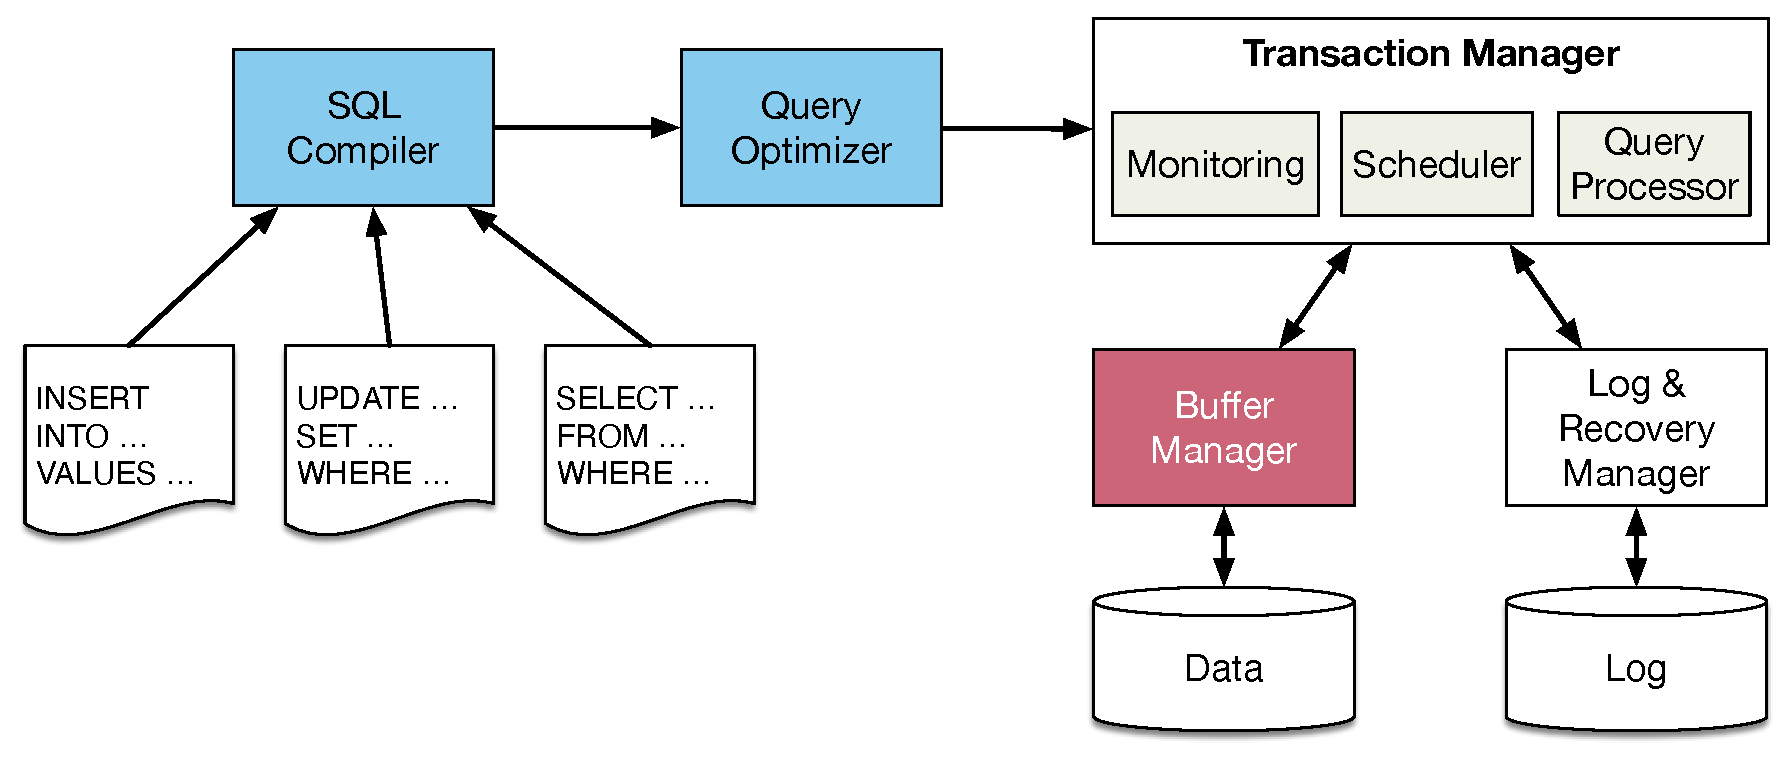
\includegraphics[width=0.8\textwidth]{../lec00_intro/figures/dbms_architecture}
\end{center}

These notes look into basic concepts from Computer Architecture (CMPUT229) and Operating Systems (CMPUT379) that relate to DBMSs and database applications.

\end{frame}

\tableofcontents

%
% ============================================================================
%
\section{Computer Architecture Basics}
%!TEX root = ./lec03_hardware.tex


%
% ---------------------------------------------------------------------------
%
\begin{frame}
\label{architecture}

Virtually all computers today, from cell phones to servers, have the same internal architecture, introduced by John Von Neumann in the 1945\footnote{\url{https://en.wikipedia.org/wiki/Von_Neumann_architecture}}.

\vskip1em

\begin{columns}[onlytextwidth]
\begin{column}{0.4\textwidth}
Both programs and data are \textbf{stored in memory}.\\[1em]
Programs are executed by the Central Processing Unit (CPU), one instruction at a time.\\[1em]
Constant move of code and data between memory and CPU.
\end{column}
\begin{column}{0.6\textwidth}
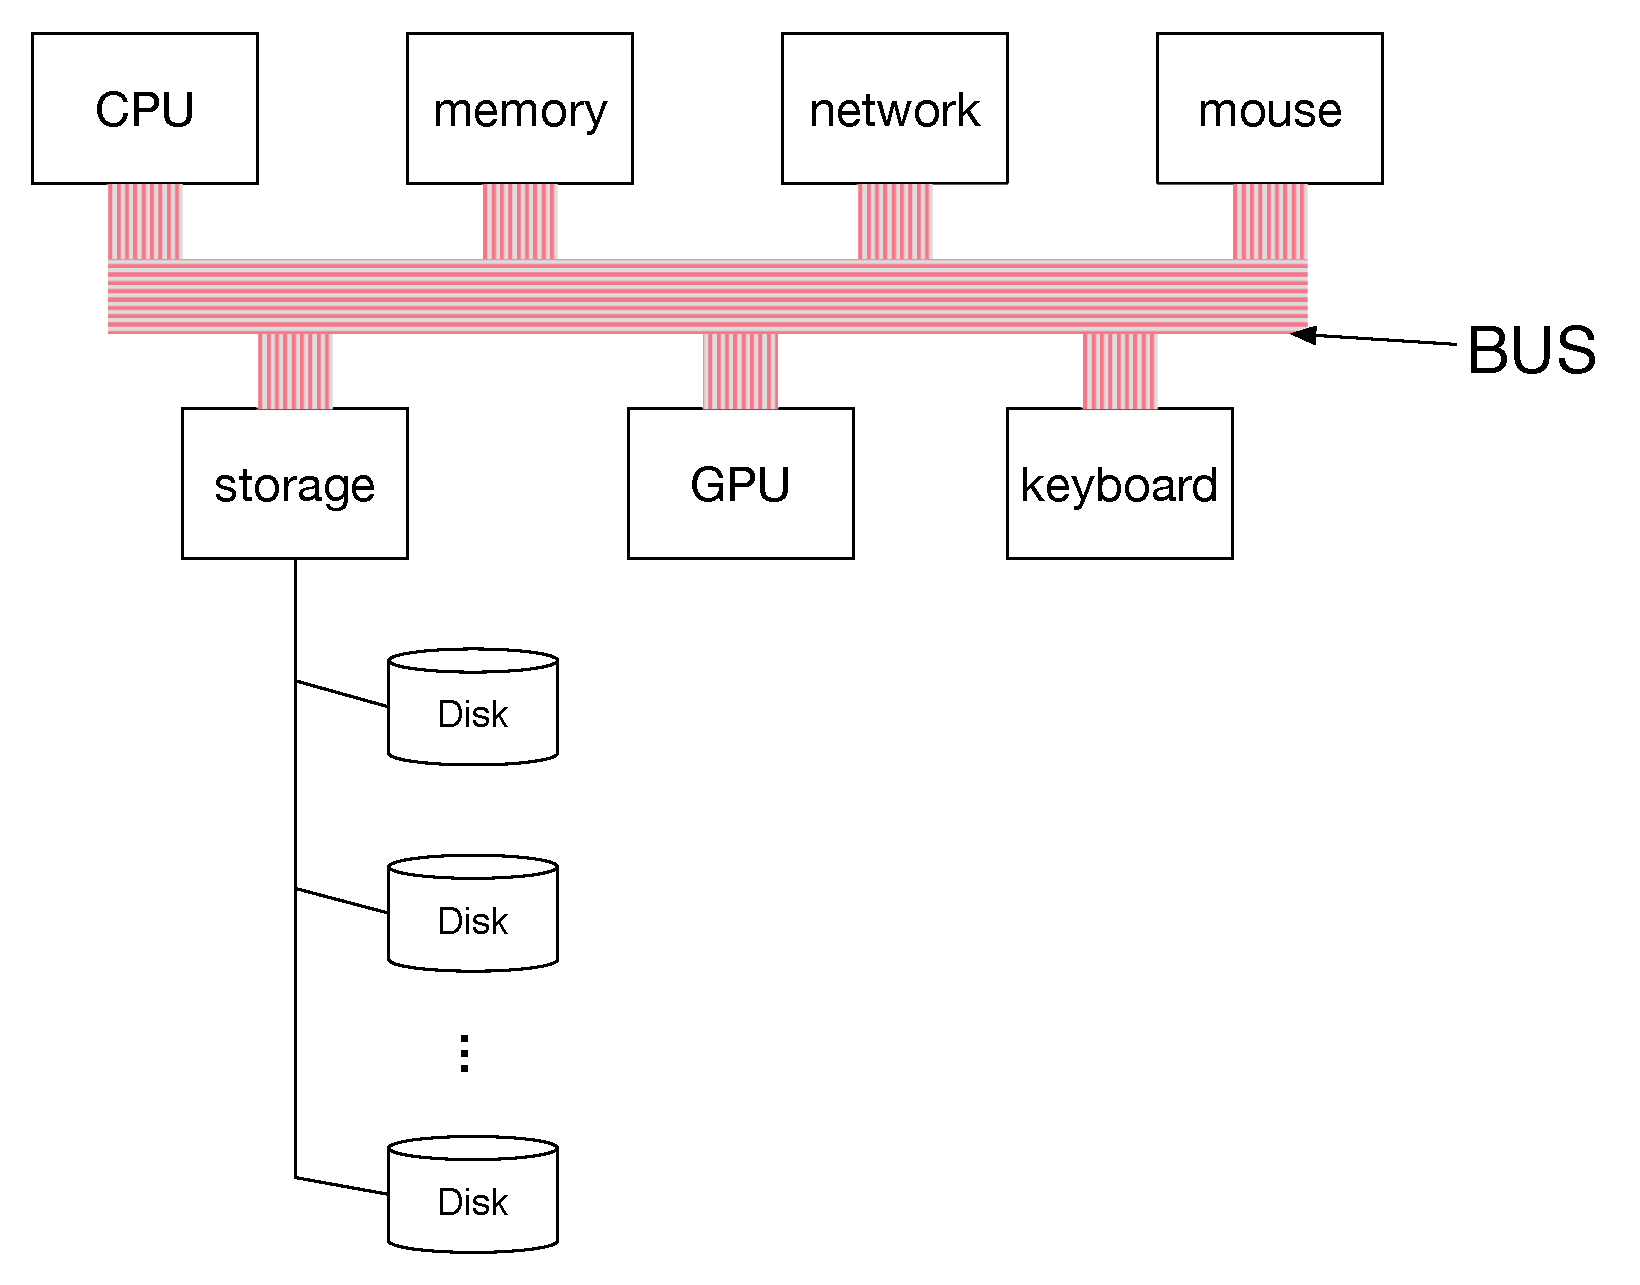
\includegraphics[width=1.1\textwidth]{./figures/von_neumann_architecture}
\end{column}
\end{columns}
\end{frame}

\begin{frame}

Components are interconnected by a Bus\footnote{\url{https://en.wikipedia.org/wiki/Bus_(computing)}}.

\begin{center}
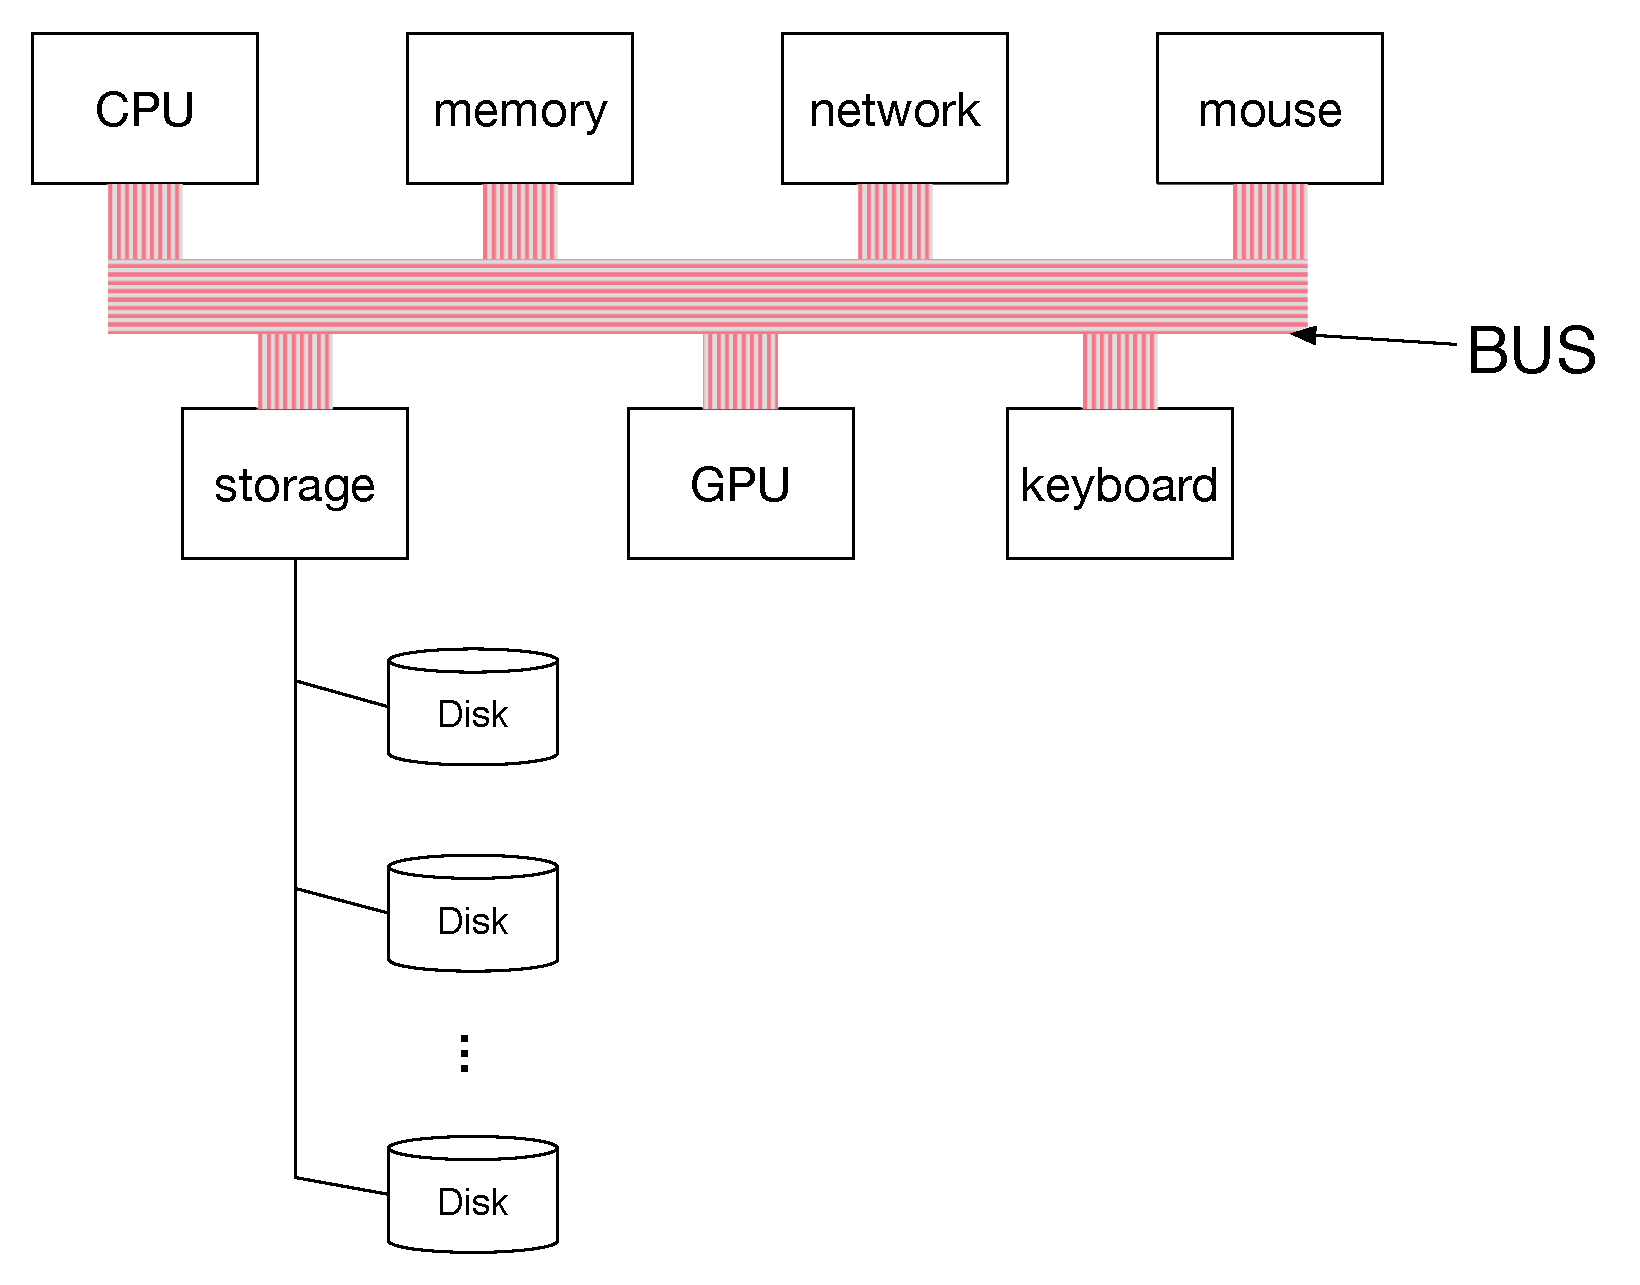
\includegraphics[trim={0 12cm 0 0},clip,width=0.65\textwidth]{./figures/von_neumann_architecture}
\end{center}

\vskip1em 

\begin{block}{The BUS \alert{must be \textbf{shared} by} all components.}
It can only be used for \textbf{unidirectional} transfers between two components at a time (e.g., from memory to the CPU).
\end{block}

% \vskip0.25em 

To maximize efficiency, transfers between \textbf{storage and memory} or \textbf{memory and CPU} are made in \alert{\textbf{fixed-sized batches}} (called \alert{memory pages} or \alert{disk blocks}).

\vskip1em 

\end{frame}

\begin{frame}

As far as the DBMS is concerned, these three components are the most important:

\begin{center}
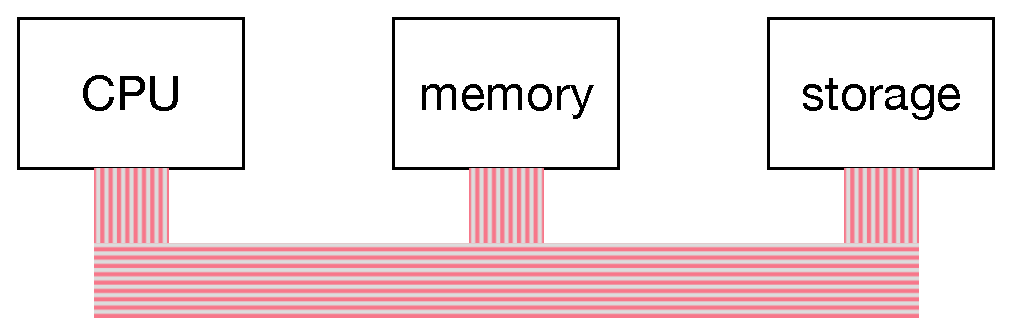
\includegraphics[width=0.5\textwidth]{figures/von_neumann_architecture_2}
\end{center}

The CPU is where the DMBS code runs (e.g., where SQL queries are executed).

The storage is where the database is stored persistently (i.e., even when the computer is off).

Memory is where the data from storage resides before it can be used by the CPU.

\end{frame}


\begin{frame}

However, the CPU does not access data in storage directly. 

\textbf{Memory-mapped I/O:} access to data on files is done by mapping those files to buffers in memory.

\vskip2em

\begin{center}
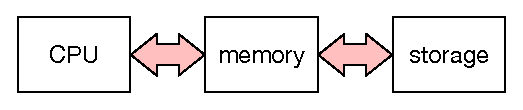
\includegraphics[width=0.5\textwidth]{figures/memory_mapped_io}
\end{center}

\vskip1em

The memory is at the center of modern architectures, so we will look at how it works first.

\end{frame}


\begin{frame}

Memory is organized as a grid of cells, each with a \underline{unique address}. 

The number of addresses depends on the computer. Typically, 32-bit computers have $2^{32}$ addresses, 64-bit computers have $2^{64}$ addresses, and so on.

\vskip1em

\begin{columns}[onlytextwidth]
\begin{column}{0.225\textwidth}
Ex: computer with \textbf{6-bit} addresses, for a memory with $2^6=64$ cells.

\vskip1em

Each cell holds a fixed-sized \textbf{word} (typically 64 bits).

\vskip1em

~
\end{column}
\begin{column}{0.75\textwidth}
\hspace*{2em}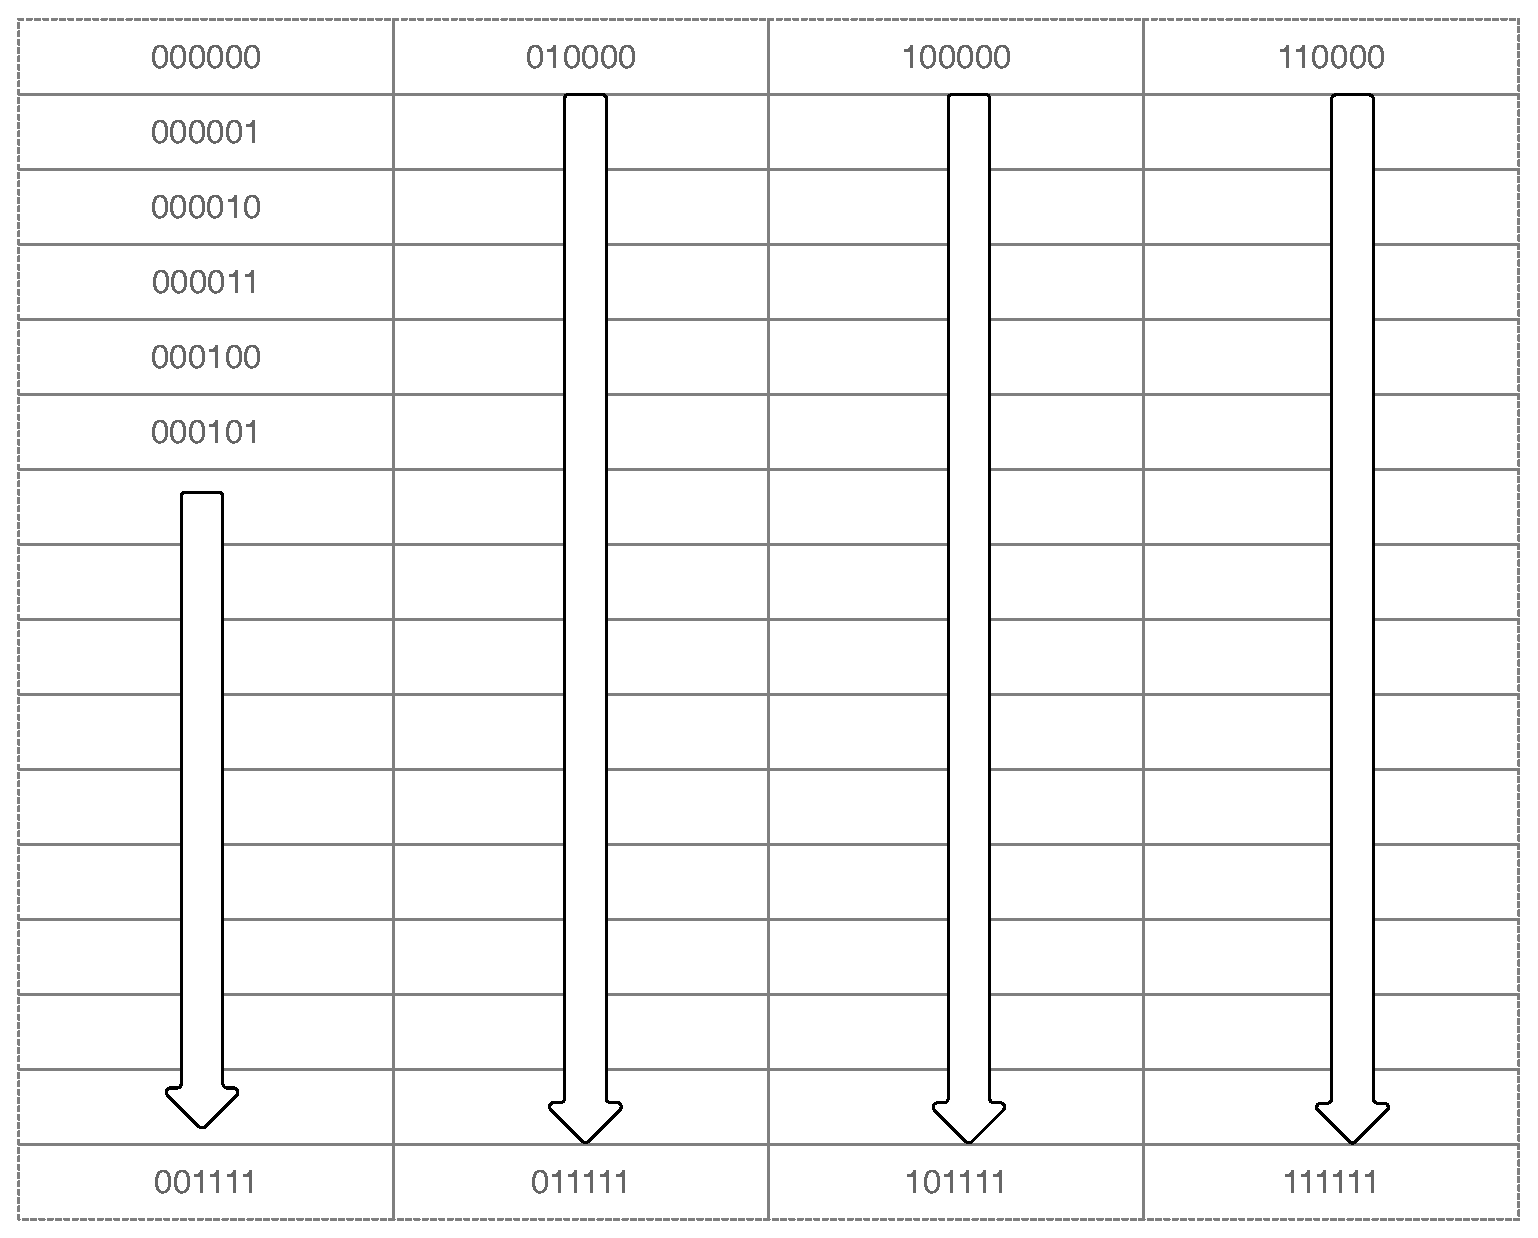
\includegraphics[width=0.9\textwidth]{figures/64_cell_memory_diagram}
\end{column}
\end{columns}
\end{frame}



\begin{frame}

The bits in the memory address are divided into two parts. Some bits are used to indicate a \textbf{page of memory}, and the other bits are used to indicate an \textbf{offset} inside the page.

\vskip1em

\begin{columns}[onlytextwidth]
\begin{column}{0.225\textwidth}
Ex: \alert{4} bits for a \alert{page} and \blue{2} bits for the \blue{offset}.

\vskip1em

So, the memory in our example is divided into $2^{\alert{4}}= \alert{16}$ pages, each with $2^{\blue{2}}=\blue{4}$ cells.
\vskip1em


\end{column}
\begin{column}{0.75\textwidth}

\begin{tikzpicture}
\node at (0,0) [anchor=south west] {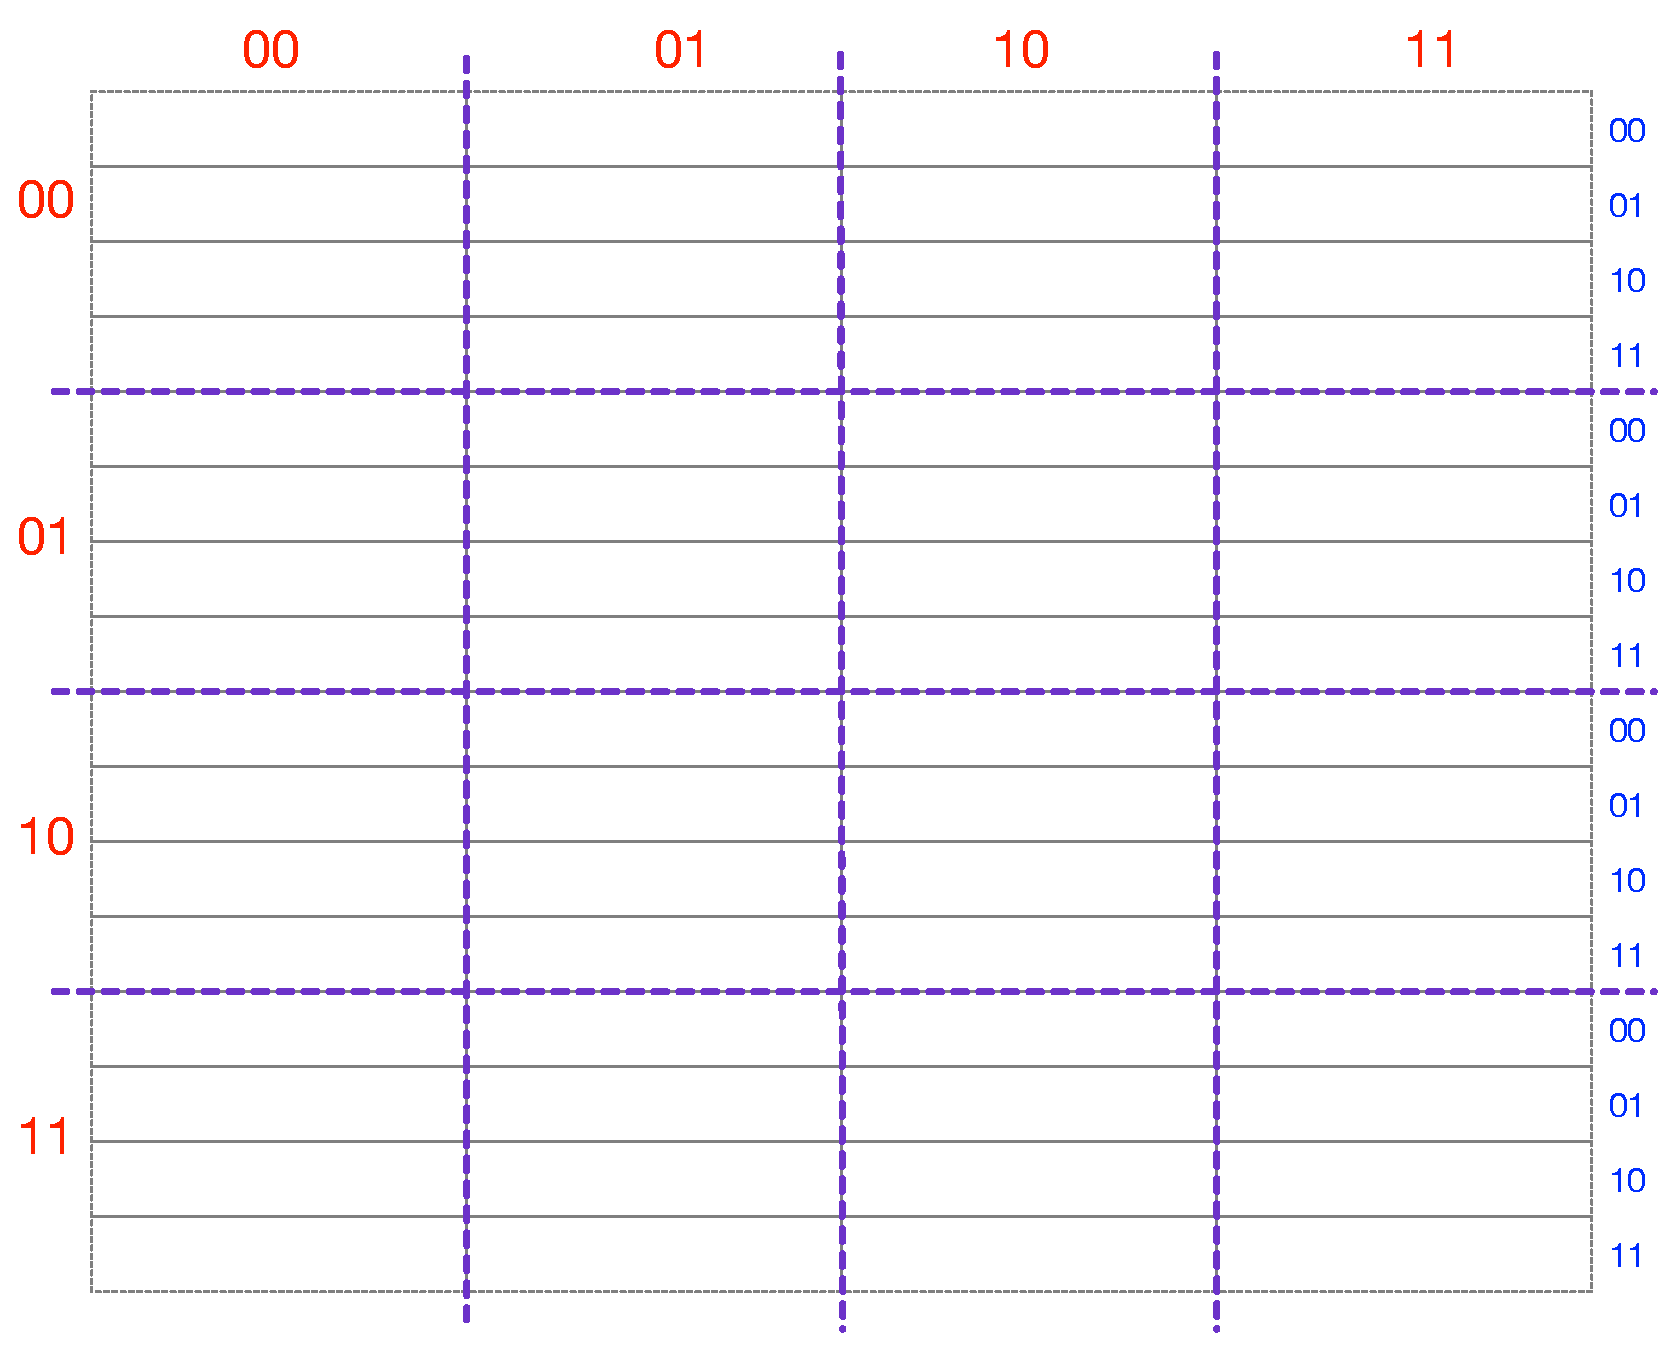
\includegraphics[width=\textwidth]{figures/6_bit_memory_grid}};
\draw[draw=red,line width=1.5pt] (4.2,3.3) rectangle ++(1.85,1.45) 
	node [fill,anchor=north east,yshift=10pt,xshift=-10pt,text=red,fill=white] {page};
\end{tikzpicture}

\end{column}
\end{columns}
\end{frame}

\newsavebox\CExample
\begin{lrbox}{\CExample}
\begin{lstlisting}[style=C]

data = (int*) malloc(20 * sizeof(int));

// initialize data array...

for (int i = 0; i < 20; i++){
    data[i] = data[i] + 1;
}
\end{lstlisting}
\end{lrbox}



\begin{frame}[fragile]

Consider a hypothetical C program:

\begin{center}
\framebox{\scalebox{0.75}{\usebox{\CExample}}}
\end{center}

The program is compiled into binary code and stored into one or more disk blocks. When the program is \underline{executed}, each block is brought to a \underline{page in memory}.

Dynamically allocated data structures are stored on (possibly many) pages in memory as well.

The local variable \lstinline[style=C]!data! is represented in the program \emph{heap} and contain the address in memory where the actual array is located.

\end{frame}


%
% ---------------------------------------------------------------------------

\newsavebox{\MemoryPagesBox}
\savebox{\MemoryPagesBox}{
	\hspace*{-1em}\begin{tikzpicture}
\node at (0,0) [anchor=south west] {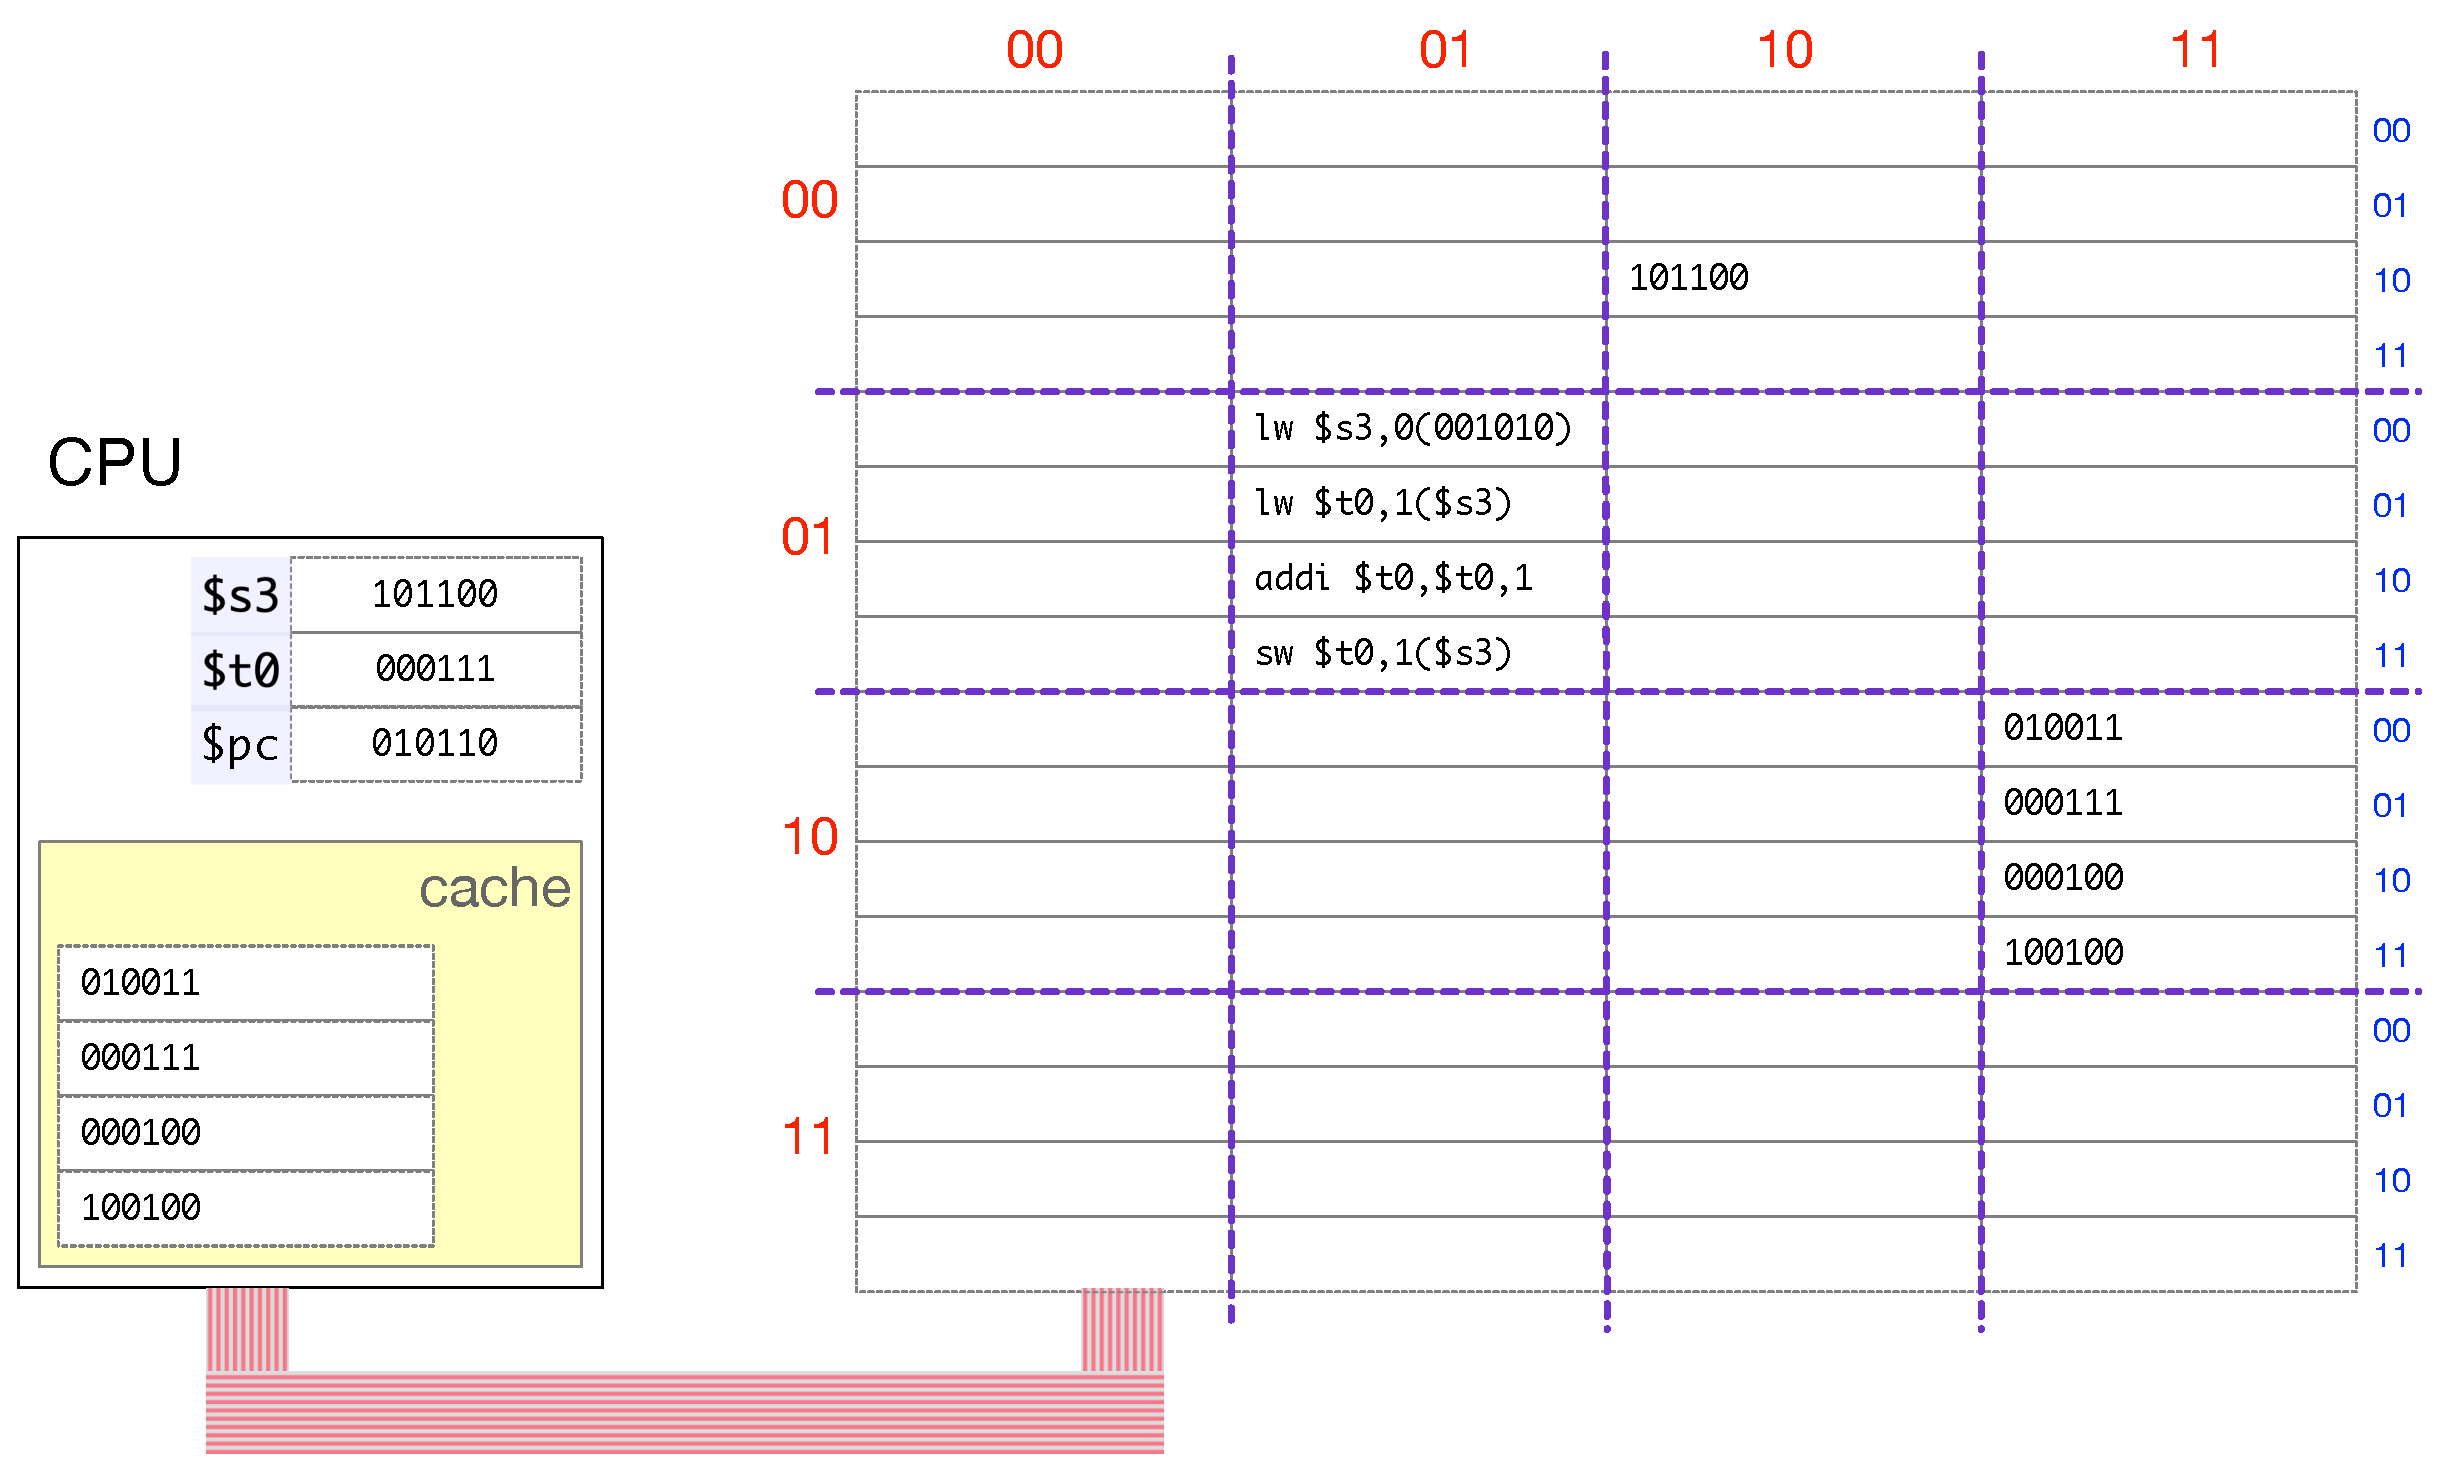
\includegraphics[width=1.2\textwidth]{./figures/CPU_memory_detailed}};
\only<1>\draw[draw=red,line width=1.5pt] (6.7,4.25) rectangle ++(2,1.6) 
	node [fill,anchor=north east,yshift=10pt,xshift=-5pt,text=red,fill=white] {program};
\only<2>\draw[draw=red,line width=1.5pt] (8.7,5.9) rectangle ++(2,1.6) 
	node [fill,anchor=north east,yshift=10pt,xshift=-12pt,text=red,fill=white] {heap};	
\only<3>\draw[draw=red,line width=1.5pt] (10.7,2.6) rectangle ++(2,1.6) 
	node [fill,anchor=north east,yshift=10pt,xshift=-12pt,text=red,fill=white] {data};
\end{tikzpicture}
}
%
\begin{frame}
\vskip1em

\begin{center}
\scalebox{0.75}{\usebox{\MemoryPagesBox}}
\end{center}

Even though the memory sends entire pages to the CPU, the \underline{program instructions use individual memory cells}.

A cache memory inside the CPU holds copies of pages in memory, from where the CPU can access the cells.

\end{frame}

%
% ---------------------------------------------------------------------------
%
\begin{frame}{The CPU}

The CPU works in \textbf{cycles}, defined by internal ticking \alert{clock} (1 GHz = 1 billion ticks per second).

Abstractly speaking, in each cycle, the CPU:\\
(1) fetches the \textbf{next}\footnote{The \textbf{program counter} (\lstinline{$pc}) register keeps the address of that instruction.} instruction of the program, \alert{from memory}\\
(2) decodes and executes the instruction \\
(3) increments the program counter to the next instruction

\begin{BOX}{Program vs CPU instructions}
Each instruction in a program in a high-level language (e.g., a \lstinline[style=C]{printf()} statement) gets compiled into many (sometimes thousands) of CPU instructions.
\end{BOX}


\end{frame}

%
% ---------------------------------------------------------------------------
%
\begin{frame}

The registers (e.g., \alert{\$s3}, \alert{\$pc}) are circuits inside the CPU that can hold the content of a \textbf{single word} in memory.

\vskip0.5em

Arithmetic (and other) operations values stored in registers:\\
 - ex: \alert{\lstinline[style=C]!addi $t0,$t0,1!} adds a constant (1) to the value in register \lstinline[style=C]{$t0}\\
 - the results of these operations are written back to registers.

\vskip1em

\begin{BOX}{The CPU \textbf{does not manipulate} memory cells directly }
instead it must move data from memory into registers (via the cache memory) and back:\\
 - ex: \textbf{load a word from memory}: \lstinline[style=cmput391]{-:lw :- <register>,<address>}\\
 - ex: \textbf{store a word into memory} : \lstinline[style=cmput391]{-:sw :- <register>, <address>}
\end{BOX}
\end{frame}


% ---------------------------------------------------------------------------

\begin{frame}{Multi-core CPUs}

Modern CPUs have many (typically, between 2 and 32) independent processors (or \textbf{cores}).

\vskip1em

\begin{columns}[onlytextwidth]
\begin{column}{0.45\textwidth}
Each core has its own private (L2) cache, but can also use a larger shared (L3) cache.

\vskip1em

Multiple programs can run at the same time, on different cores.
\end{column}
\begin{column}{0.5\textwidth}
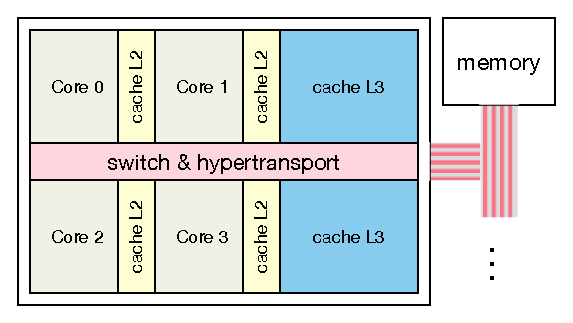
\includegraphics[width=1.1\textwidth]{figures/multicoreCPU.eps}
\end{column}
\end{columns}

\vskip0.5em

Moreover, the same program can be broken into multiple processes (also called \emph{threads}) which can run \textbf{at the same time} on different cores.

\end{frame}


%
% ---------------------------------------------------------------------------
%
\begin{frame}{Volatile and persistent memory}

\begin{columns}[onlytextwidth]
\begin{column}{0.475\textwidth}
\begin{BOX}{Volatile Memory}
Memory that needs continuous power to keep its contents. Also called \emph{transient} memory.\\[1em]
Ex: registers, caches, \alert{RAM}
\end{BOX}
\end{column}
\begin{column}{0.475\textwidth}
\begin{BOX}{Persistent Memory}
Memory that keeps its contents even without continuous power.\\ \alert{Also known as \emph{storage}}.\\[1em]
Ex: HDDs and SSDs
\end{BOX}
\end{column}
\end{columns}

\vskip1em

The \alert{``main memory''} refers to RAM (Random Access Memory) circuits that are much larger (and much slower) than the CPU caches.

\end{frame}



%
% ---------------------------------------------------------------------------
%
\begin{frame}{Compared to main memory... \alert{storage is very slow}...}

Many reasons:
\begin{itemize}[-]
\item Reliable media that is (1) rewritable, (2) persistent and (3) affordable is also slow (compared to even DRAM).

\item \textbf{Error-correction}: to prevent data loss, devices check everything that has been read or written against error correction codes (e.g., hash values), which takes time.

\item \textbf{Synchronization}: data can only be transferred between the device and memory when the data BUS is not in use.

\item Some devices have mechanical parts that are orders of magnitude slower than electronic components.

\end{itemize}

\end{frame}

%
% ---------------------------------------------------------------------------
%
\begin{frame}
\vskip2em
\begin{columns}
\begin{column}{0.5\textwidth}
Hard Disk Drives (HDD) store data on the surface of spinning disks (platters). Many drives have 2 or more disks.
\begin{itemize}[-,topsep=-0.1em]
 \item data is read or written by a ``head'' traveling close to (but never touching) the platter

 \item data are stored on circular \emph{tracks} on the platter

 \item with multiple platters, a \emph{cylinder} is formed by all tracks at the same distance from the spindle

 \item each track/cylinder is divided into \emph{sectors}
\end{itemize}
\end{column}
\begin{column}{0.45\textwidth}
\hspace*{-1em}
\centering
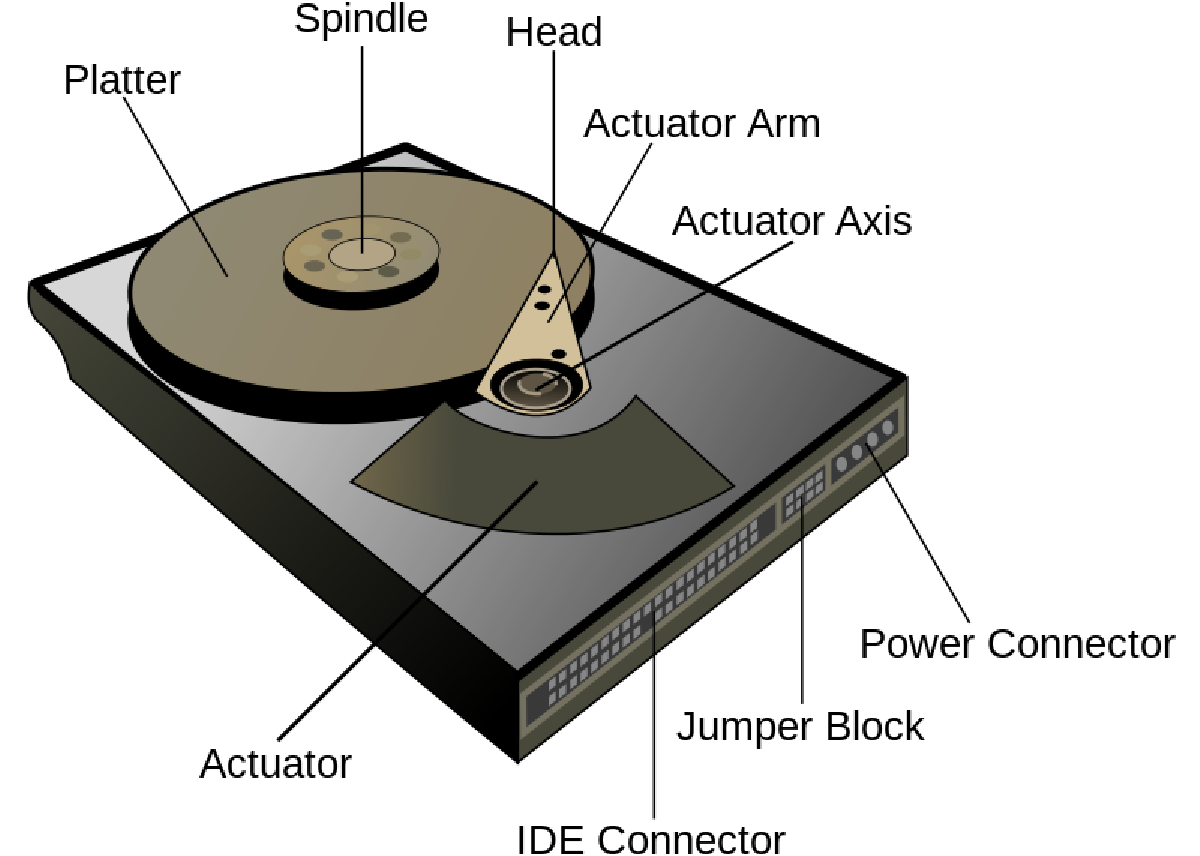
\includegraphics[width=1.2\textwidth]{figures/800px-Hard_drive-en}

\vskip1em

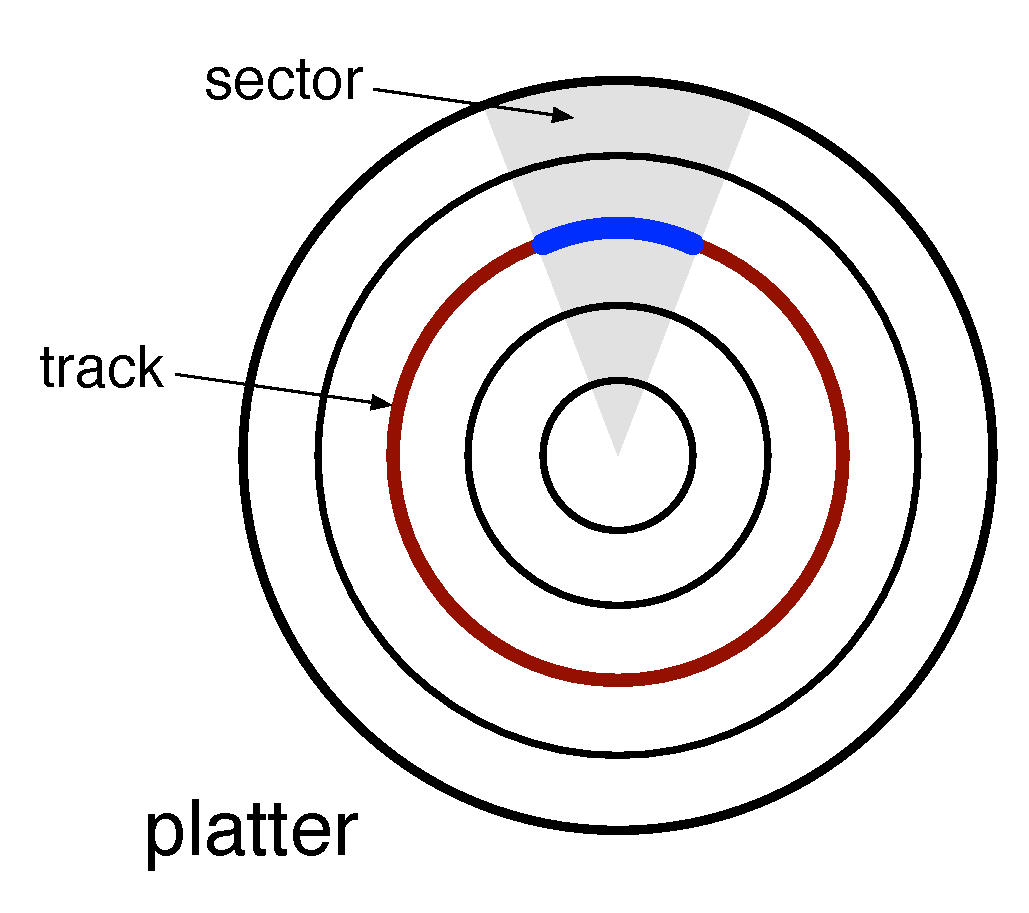
\includegraphics[width=0.7\textwidth]{figures/HDD_sector_track}
\end{column}
\end{columns}
\end{frame}
%
% ---------------------------------------------------------------------------
%
\begin{frame}
\vskip1em
\begin{BOX}{HDD Seek Time}
Time until the actuator arm moves to the desired track.

- \emph{in expectation}: average time to travel between any two tracks;

- \emph{typical}: between 3ms to 13ms

\vskip1em

\textbf{Data locality}: the seek time between \emph{adjacent} tracks is very short.
\end{BOX}

 \vskip0.5em

\begin{BOX}{HDD Rotational delay}
Time until the desired sector arrives under the head.

- \emph{in expectation}: time for a half-rotation of the disk;
\end{BOX}

\vskip1em
\begin{columns}
\begin{column}{0.4\textwidth}
\vskip0.5em
Practice: rotational delay of a 5400rpm disk?
\end{column}
\begin{column}{0.5\textwidth}
\[\frac{0.5 r}{5400 rpm / (60s/m)} = 5.6ms\]
\end{column}
\end{columns}
\end{frame}

%
% ---------------------------------------------------------------------------
%
\begin{frame}{Data transfer between memory and storage}

Data moves between memory and storage in \textbf{fixed-sized} chunks, called \highlight{blocks}.\\
- the block size is a system parameter configured when the device is formatted\\
- the smallest possible block size with a HDD is a single sector;\\
- \emph{typical} sizes are 4KB or 8KB.

\begin{columns}
\begin{column}{0.35\textwidth}
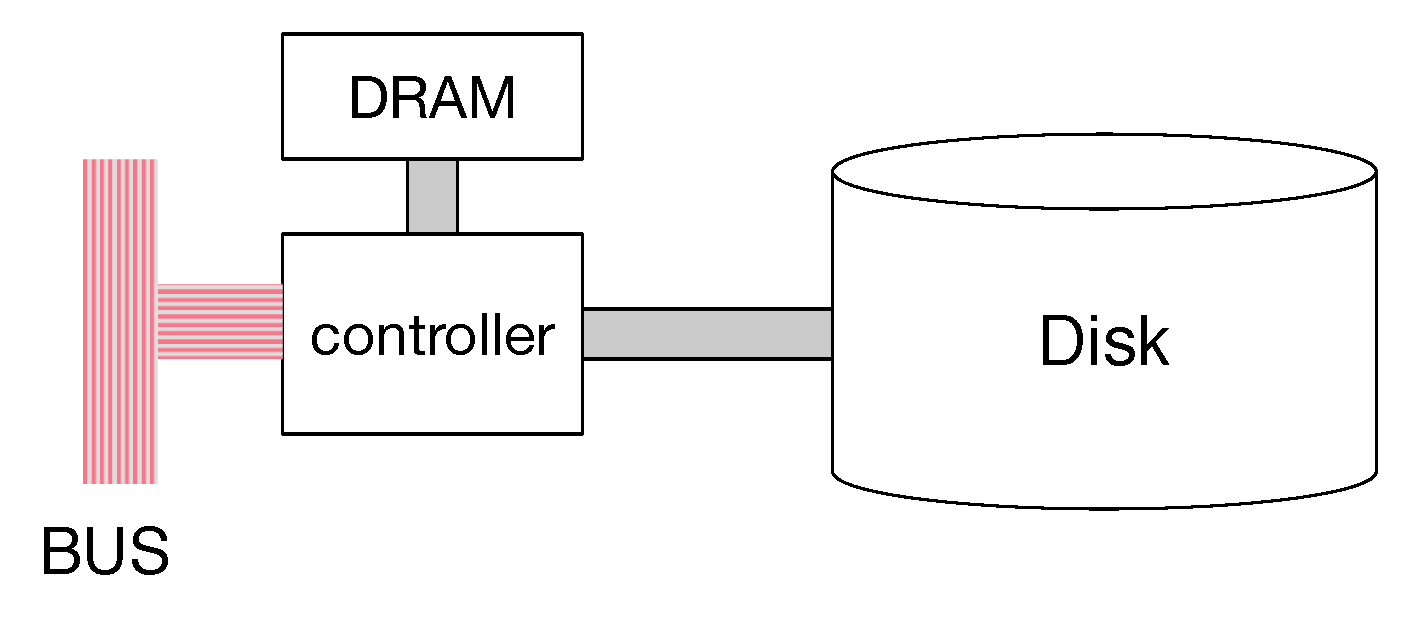
\includegraphics[width=1.1\textwidth]{figures/HDD_architecture}
\end{column}
\begin{column}{0.35\textwidth}
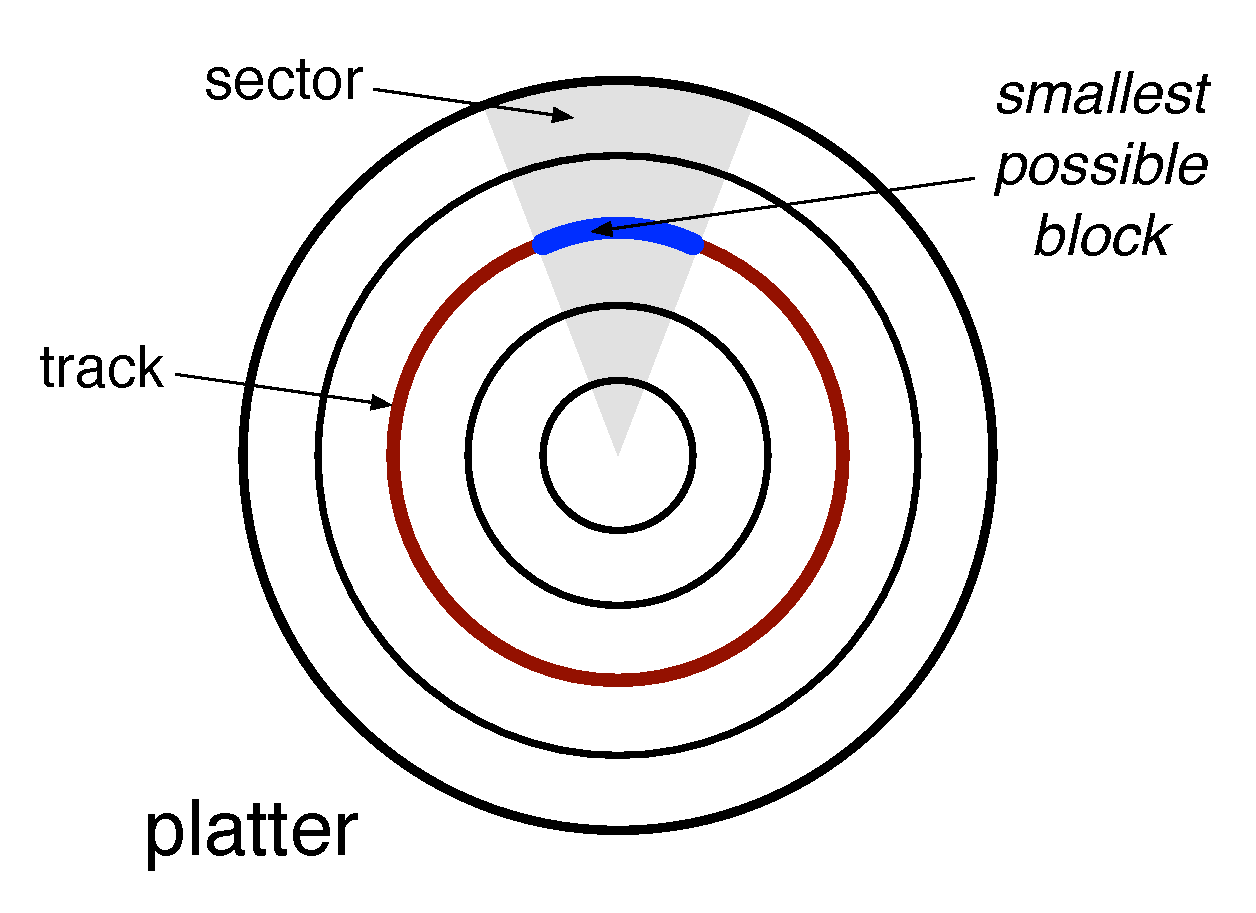
\includegraphics[width=\textwidth]{figures/HDD_block_size}
\end{column}
\end{columns}

In a modern HDD, the controller has an internal, (volatile) DRAM cache, typically of a few MB, which it uses to mediate data transfers with main memory.

\end{frame}

%
% ---------------------------------------------------------------------------
%

\begin{frame}
Solid State Drives (SSDs) have the same architecture as HDDs:

\vskip1em

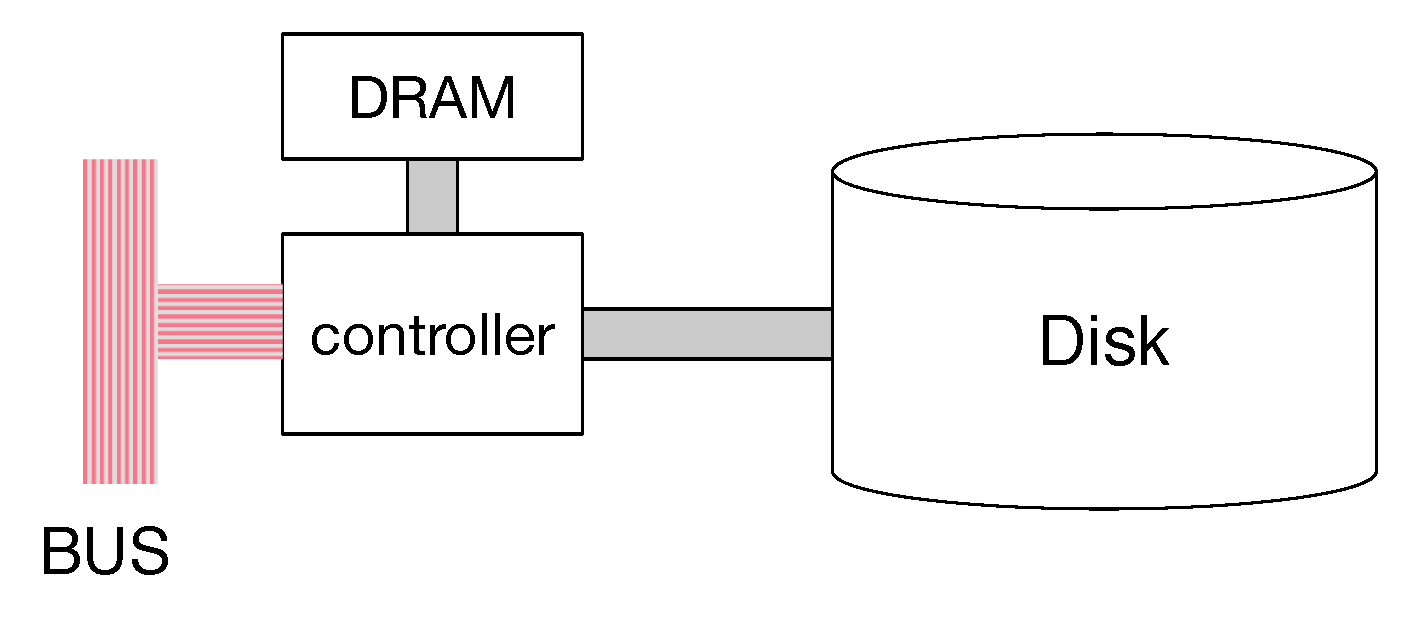
\includegraphics[width=0.45\textwidth]{figures/HDD_architecture}
~~~
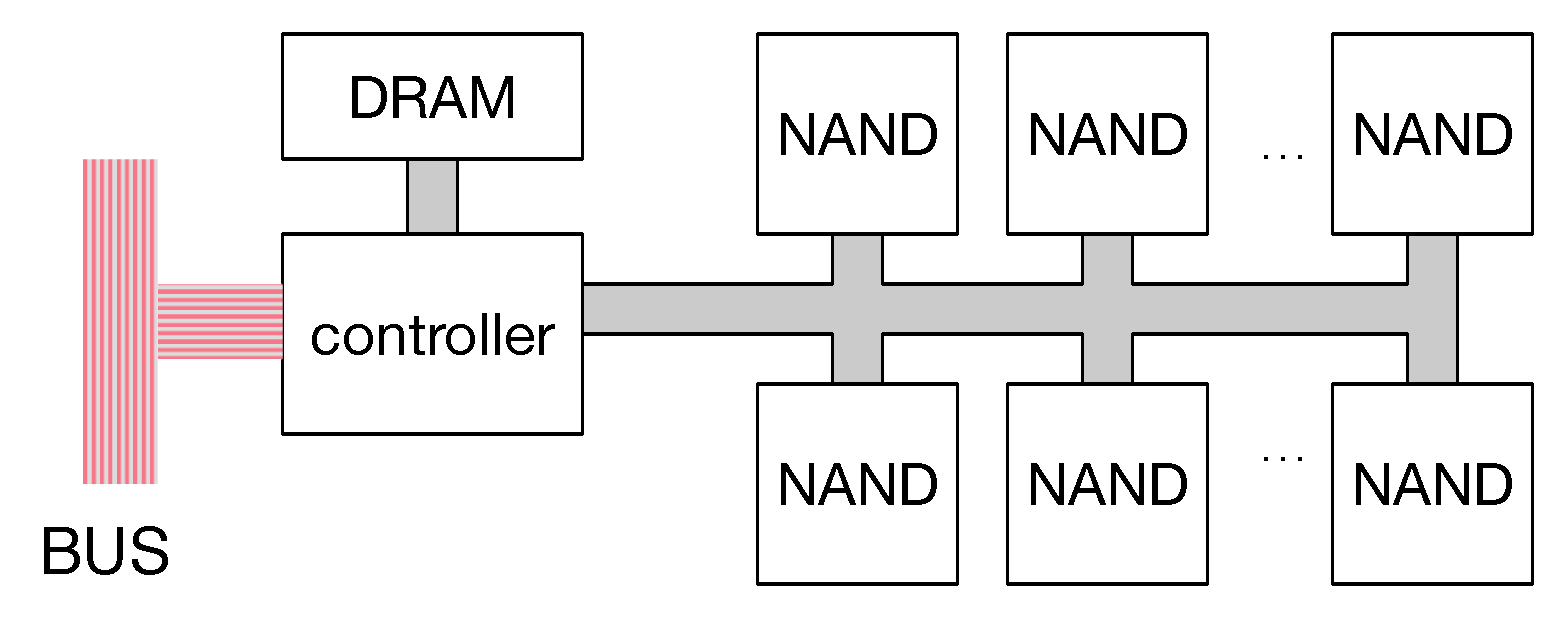
\includegraphics[width=0.45\textwidth]{figures/SSD_architecture}

\vskip1em

Even though they use a much faster medium (NAND) and have no mechanical parts, they are still block-oriented storage devices.
\end{frame}

%
% ---------------------------------------------------------------------------
%
\begin{frame}

RAID (Redundant Arrays of Inexpensive Disks) group multiple disks into a single logical storage device:

\vskip1em

\begin{center}
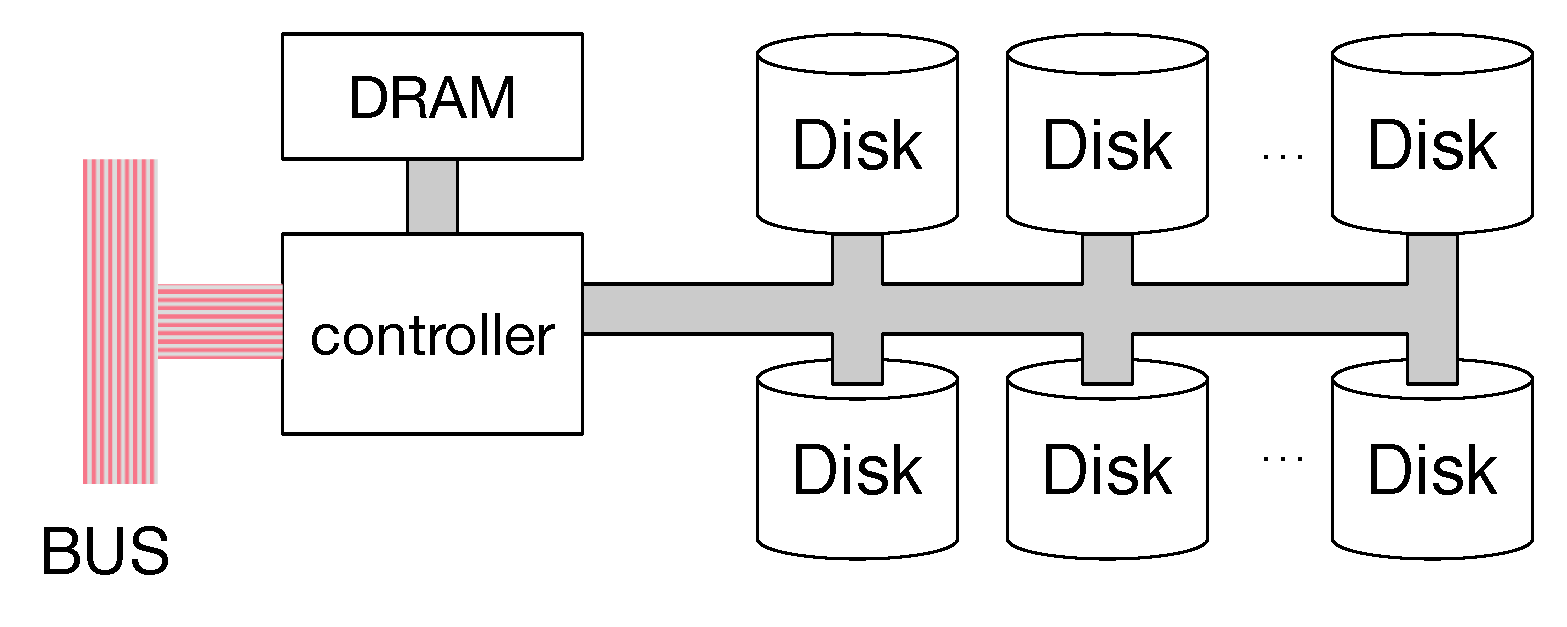
\includegraphics[width=0.45\textwidth]{figures/RAID_architecture}
\end{center}

\vskip1em

Typical RAID settings\footnote{There are many ways of configuring RAID systems.} store the same (logical) block in more than one disk. This yields higher performance and error recovery:
\begin{itemize}[-,topsep=-0.1em]
\item Each block can be read from any disk containing it;\\
\item If one disk crashes, its blocks can be read from another disk.
\end{itemize}
\end{frame}

%
% ---------------------------------------------------------------------------
%
\begin{frame}{Storage is block oriented}
\label{block_oriented_storage}

The Operating System abstracts all storage devices (HDDs, SDDs, RAID arrays, etc.) as a collection of blocks:\\
 - each block has an address;\\
 - file (names) are associated to blocks by the OS

\vskip1em

 \begin{center}
 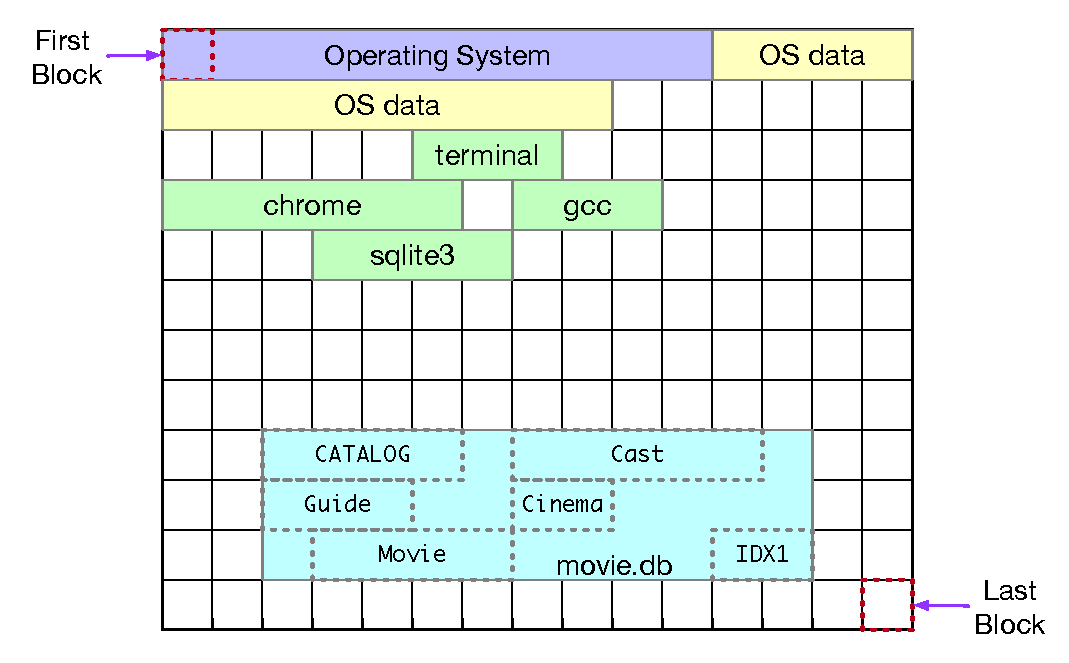
\includegraphics[width=0.75\textwidth]{figures/blocks_on_storage.eps}
 \end{center}

\end{frame}

%
% ---------------------------------------------------------------------------
%



%
% ---------------------------------------------------------------------------
%
\begin{frame}
There are two main costs when using storage:\\
- \textbf{access time}: setting the device to read/write the desired block;\\
- \textbf{transfer time}: moving data between \emph{primary memory} and the device's internal cache.\footnote{The time to move data inside the device is usually ignored.}

\vskip1em

\begin{BOX}{Access times}
- For SSDs and RAID stores, the access time is negligible (and usually very hard to model)\\
- For HDDs, access times are:

\begin{itemize}
\item[\textbf{read}:] average seek time + 0.5 rotational delay
\item[\textbf{write}:] average seek time + 1.5 rotational delay\footnotemark
\end{itemize}
\end{BOX}
\footnotetext{To verify the data was correctly written.}
\end{frame}


%
% ---------------------------------------------------------------------------
%
\begin{frame}{Memory Hierarchy}
\begin{columns}
\begin{column}{0.8\textwidth}

The ``memory'' of a computer is complex and layered sub-system comprising persistent storage, RAM, caches, and registers.

\vskip1em

\begin{BOX}{Cost/Speed}
The closer to the CPU, the faster and more expensive the memory is.
\end{BOX}


\vskip1em

\begin{minipage}{\textwidth}
\footnotesize
\begin{tabular}{l|l|c|c}
\hline
\multirow{2}{*}{\textbf{component}} & \multirow{2}{*}{\textbf{technology}} & \textbf{access} & \textbf{\$/GB} \\
& & \textbf{time (ns)} & \textbf{(2012)}\\
\hline\hline
cache & SRAM & 0.5--2.5 & 500--700\\
\hline
main memory & DRAM & 50--70 & 10--20\\
\hline\hline
\multirow{2}{*}{storage} & flash & 5E3--5E4 & 0.75--1.00 \\
\cline{2-4}
& disk & 5E6 -- 2E7 & 0.05 -- 0.10\\
\hline
\end{tabular}
\vskip1em
\hfill [Patterson \& Hennessy 2014]
\end{minipage}
\end{column}
\begin{column}{0.2\textwidth}
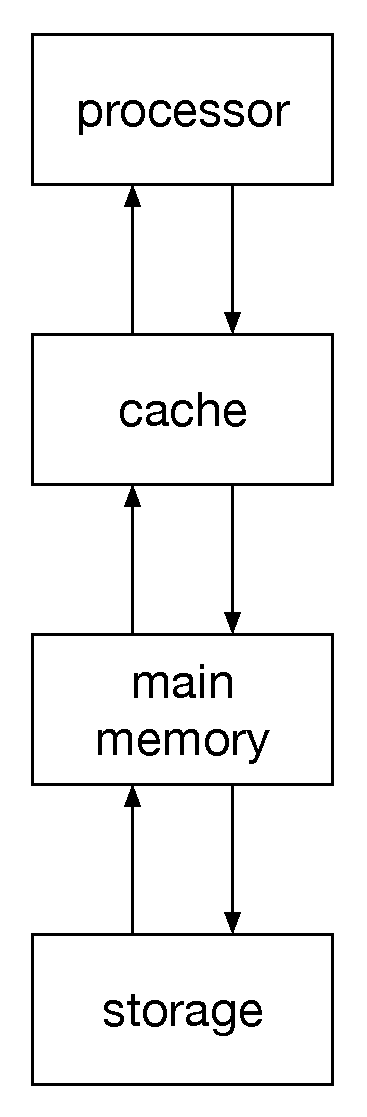
\includegraphics[width=0.8\textwidth]{./figures/memory_hierarchy}
\end{column}
\end{columns}
\end{frame}


%
% ---------------------------------------------------------------------------
%
% \begin{frame}

% \begin{columns}
% \begin{column}{0.8\textwidth}

% When the CPU needs to read a memory cell:\\
% (1) it first checks if the cell is already in the cache;\\
% (2) if not (called a \emph{cache miss}), the cell is requested from main memory

% \vskip1em

% Data comes from memory to the cache in large chunks, to minimize the chance of another cache miss in the very next instruction\footnotemark.

% \vskip2em
% \begin{BOX}{Cache misses waste CPU cycles}
% \textbf{No computation} happens during a cache miss, which must be \emph{avoided} at all costs.
% \end{BOX}

% \end{column}
% \begin{column}{0.2\textwidth}
% 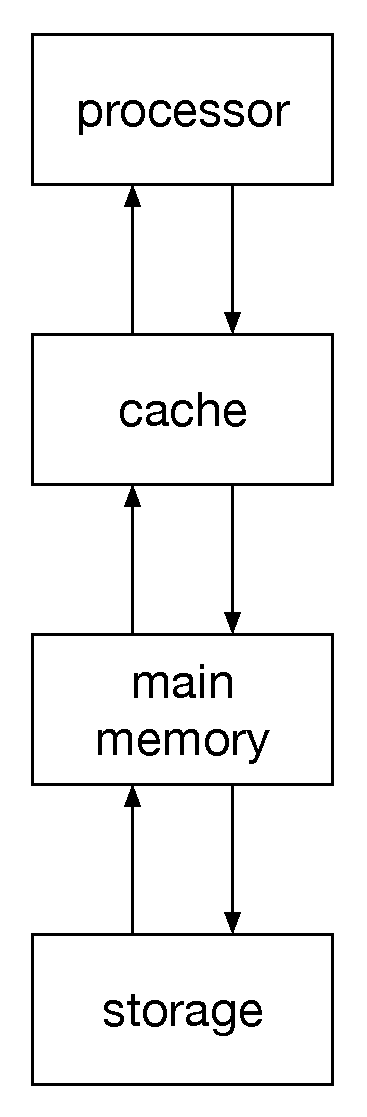
\includegraphics[width=0.8\textwidth]{./figures/memory_hierarchy}
% \end{column}
% \end{columns}

% \footnotetext{The property that a program is likely to use adjacent memory cells in a short period of time is called \emph{locality}.}

% \end{frame}

%
% ---------------------------------------------------------------------------
%
% \begin{frame}

% \begin{columns}
% \begin{column}{0.5\textwidth}
% \textbf{Data Hungry CPUs:}

% How many instructions could a Core i7-3820 execute during the time 4KB of data are transferred from disk to memory?

% \end{column}
% \begin{column}{0.5\textwidth}
% \begin{block}{Intel Core i7-3820 CPU}
% \small
% - 4 processors working at 3.6GHz

% - can theoretically execute up to \(4 \times 3.6 = 14.4\) \textbf{billion} instructions every second

% - it's DMI bus supports up to 2GB/s 
% \end{block}
% \end{column}
% \end{columns}

% \vskip1em

% \begin{BOX}{Program vs CPU instructions}
% Each instruction in a program in a high-level language (e.g., a \lstinline{printf()} statement) gets compiled into many (sometimes thousands) of CPU instructions. Nevertheless, a computer with many fast cores is bound to waste many ``idle'' cycles while data gets transferred from memory.
% \end{BOX}

% \end{frame}


%
% ============================================================================
%
\section{Virtual Memory}
%!TEX root = ./lec03_hardware.tex

%
% ---------------------------------------------------------------------------
%
\begin{frame}{Virtual Memory}
\label{virtual_memory}

Virtual Memory\footnote{\url{https://en.wikipedia.org/wiki/Virtual_memory}} is a powerful programming metaphor that allows the efficient and secure simultaneous execution of multiple programs in the same computer.

\begin{columns}[onlytextwidth]
\begin{column}{0.7\textwidth}

Each program is allowed to use virtually every memory address possible in the computer (e.g., $2^{64}$ addresses in a 64-bit machine).

\vskip0.5em

If the program requires more memory (pages) than is \emph{physically available}, the operating system automatically moves some memory pages to disk, making room for the new requests.

\end{column}
\begin{column}{0.3\textwidth}
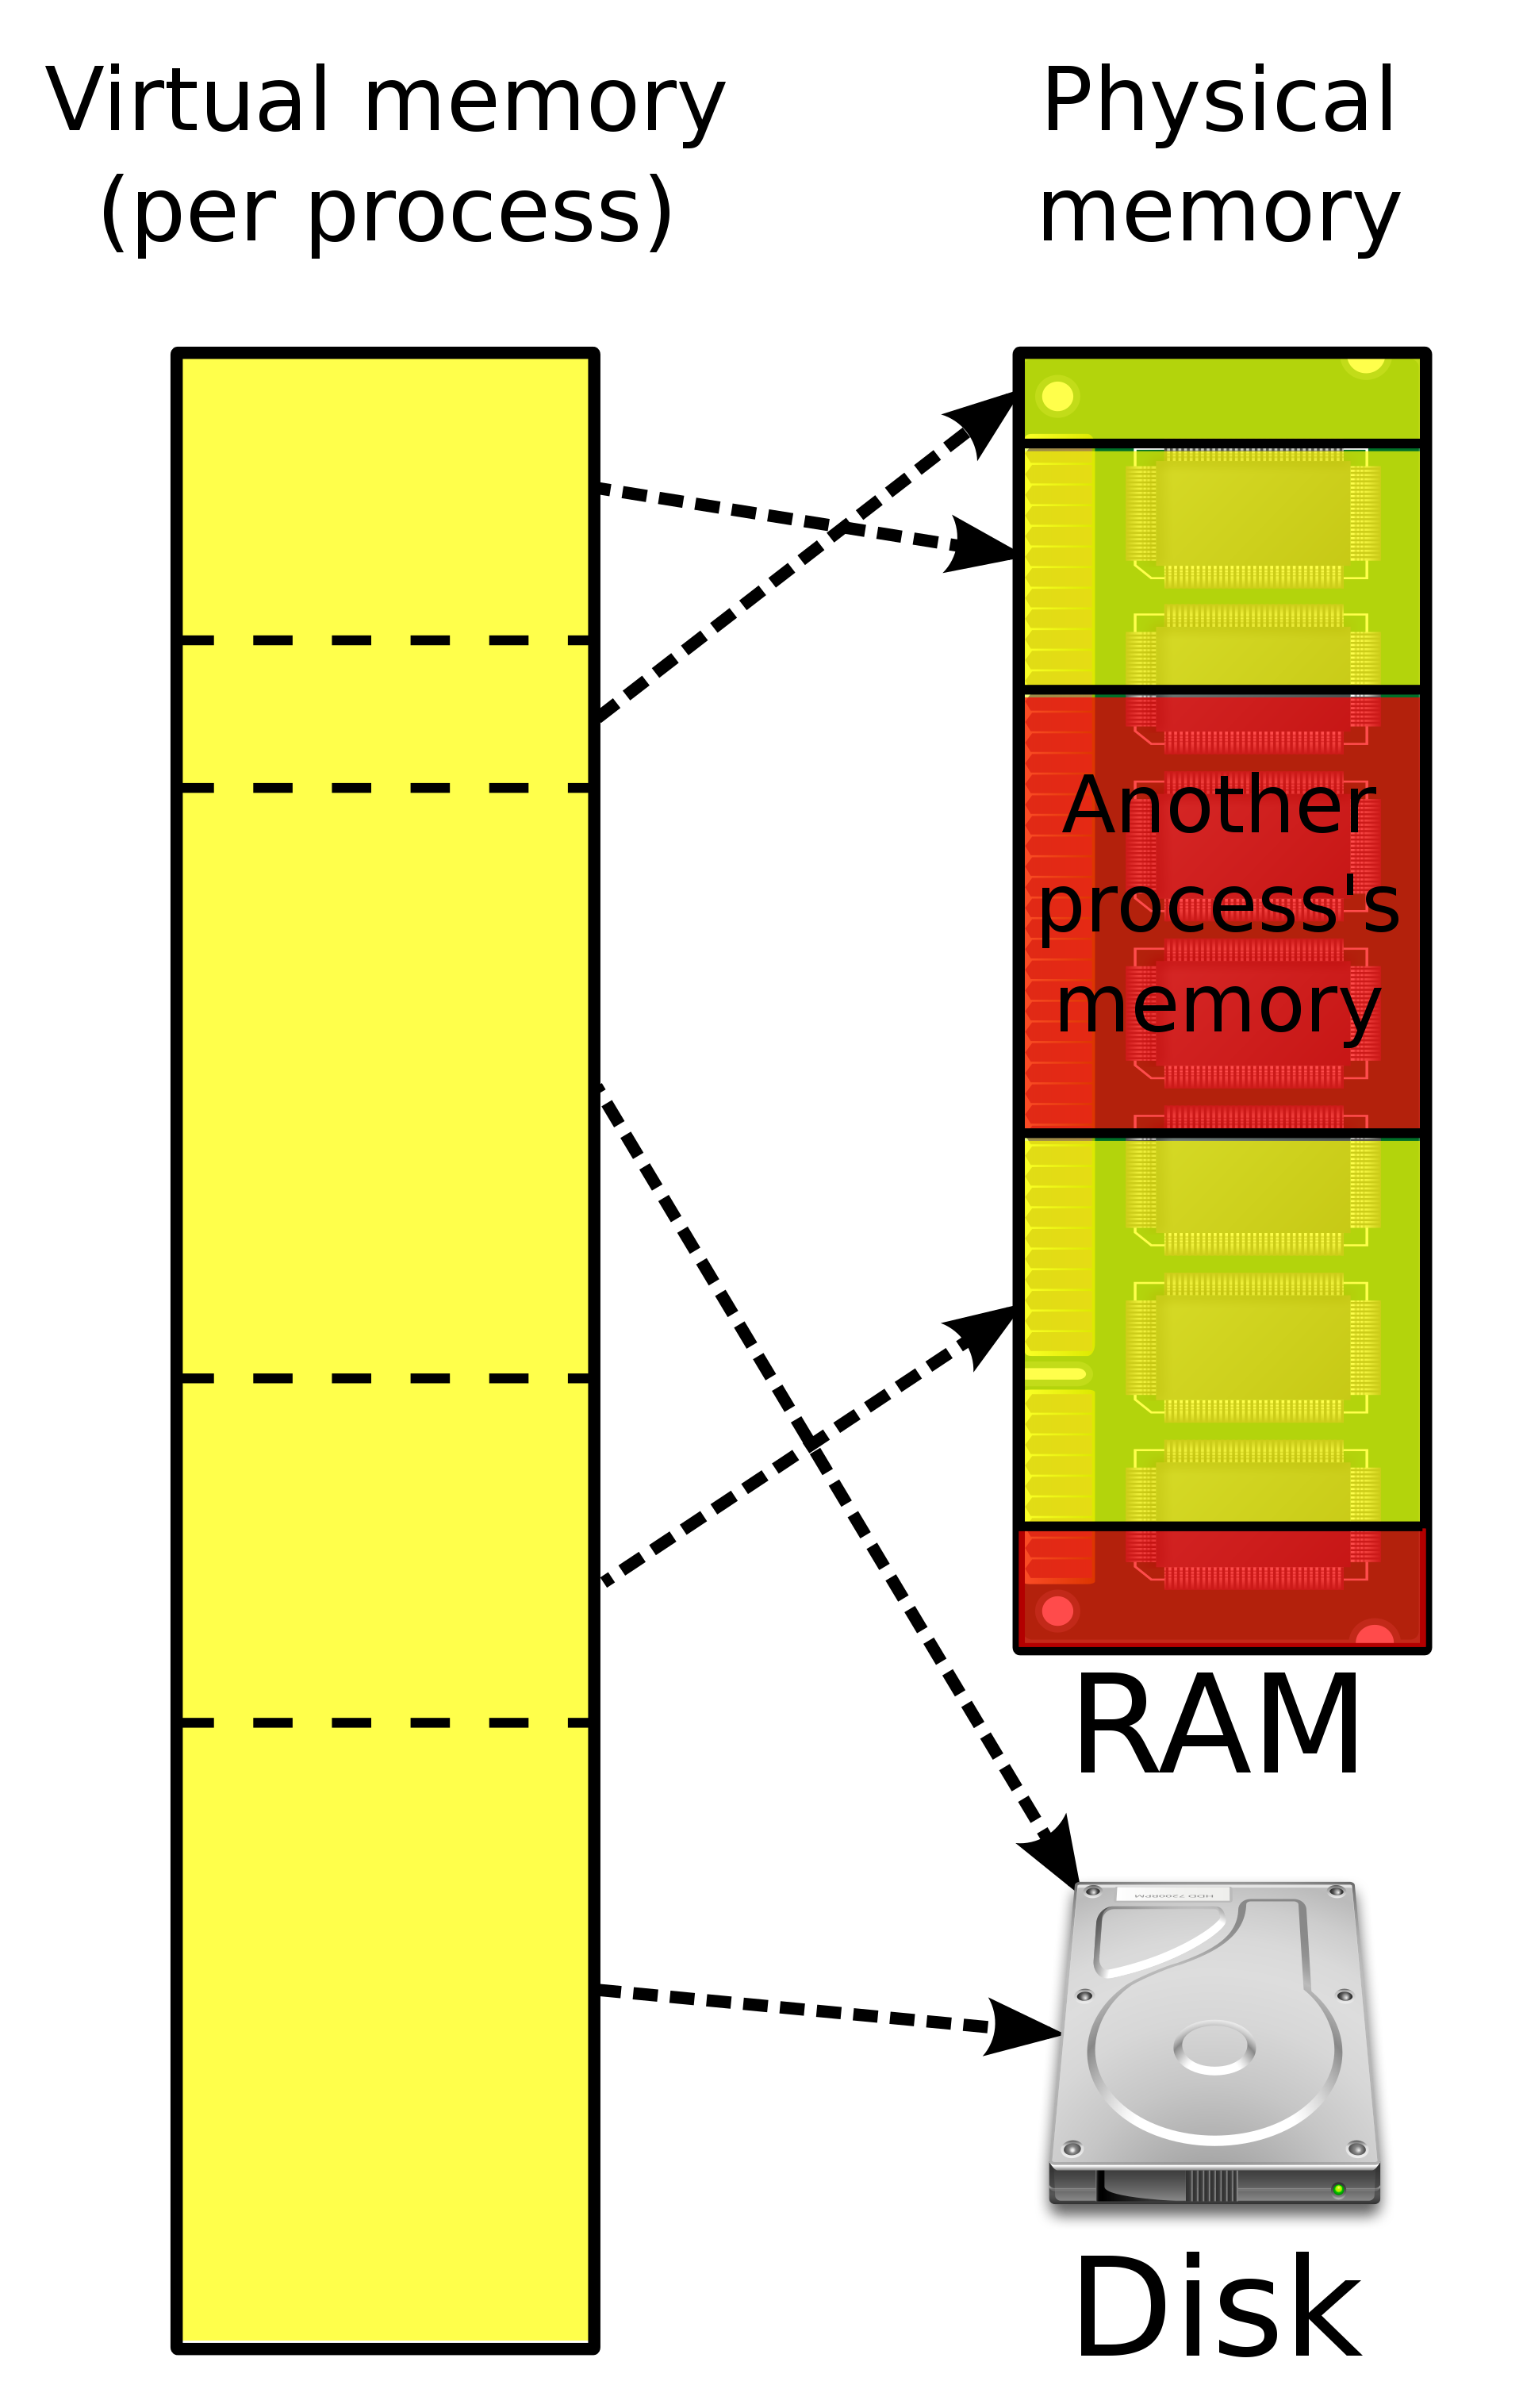
\includegraphics[width=0.9\textwidth]{figures/1920px-Virtual_memory.png}

\hfill{\tiny Source: Wikipedia.}
\end{column}
\end{columns}
\end{frame}


%
% ---------------------------------------------------------------------------
%
\begin{frame}

Programs can use all possible memory addresses (e.g., $2^{64}$ addresses on a 64-bit machine). As a result, virtual memory can have more pages than what is available in physical memory.

\vskip1em

\begin{center}
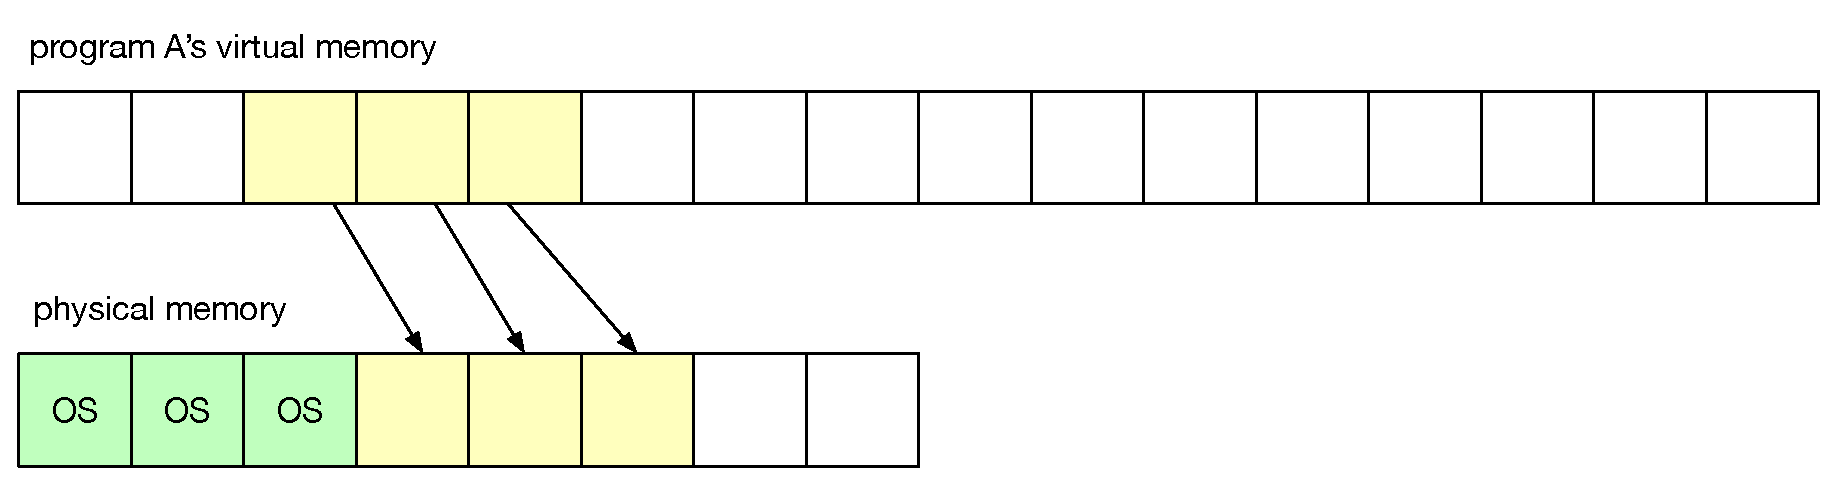
\includegraphics[width=\textwidth]{figures/virtual_memory_scene1.eps}
\end{center}

\vskip1em

As the program requests more memory, the Operating System (OS) assigns physical pages to the virtual pages of the program.

\end{frame}

%
% ---------------------------------------------------------------------------
%

\begin{frame}

Physical memory is shared by all programs in execution, including the OS itself.

\vskip1em

\begin{center}
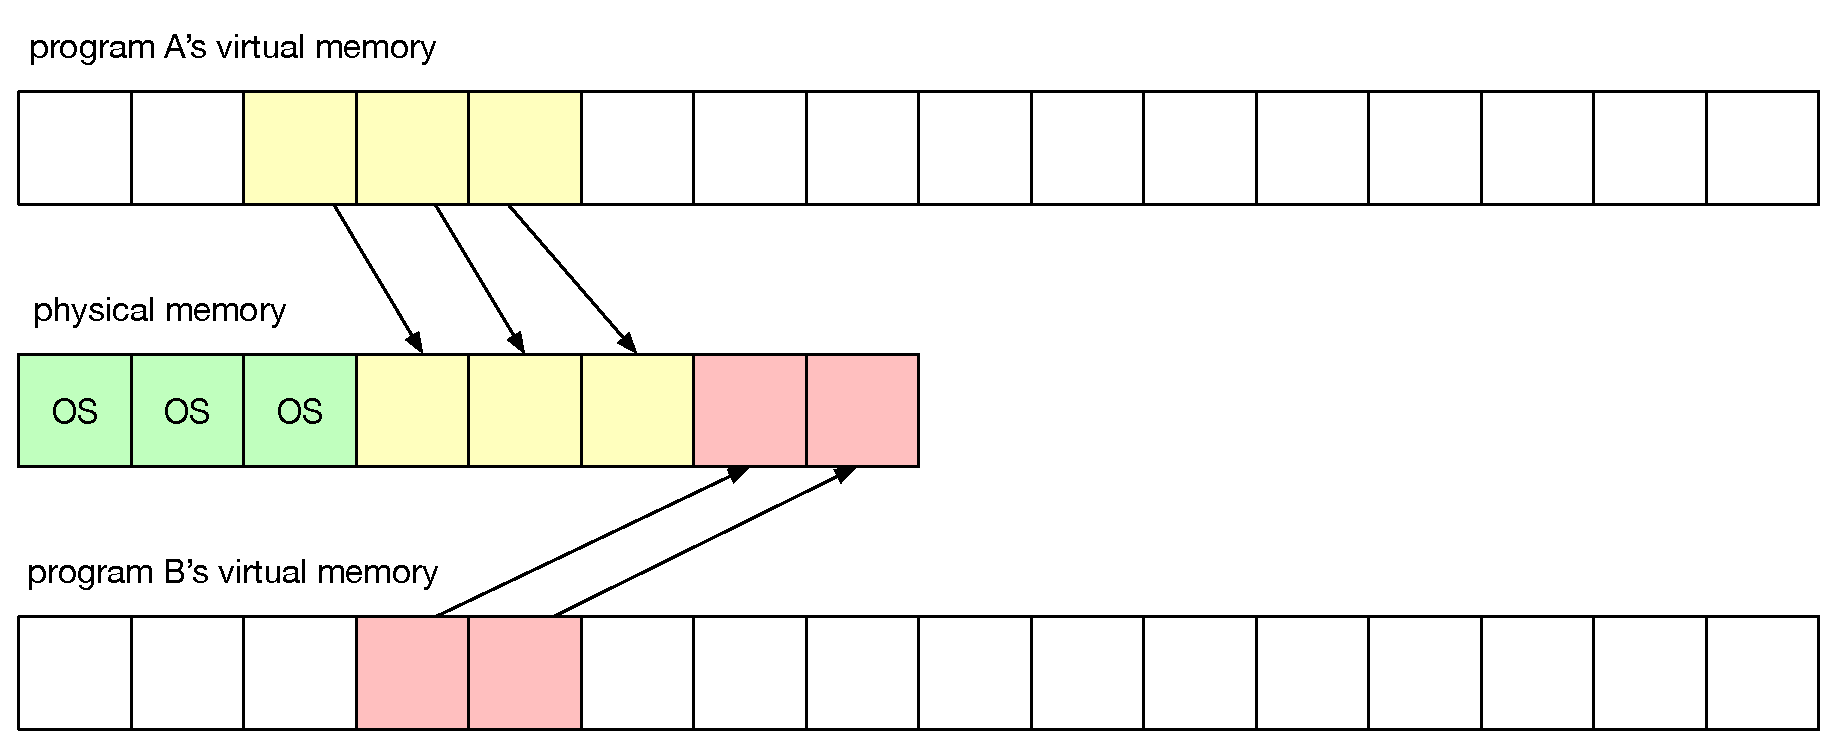
\includegraphics[width=\textwidth]{figures/virtual_memory_scene2.eps}
\end{center}

\vskip1em

Note that two different programs can have pages in the same virtual address, each mapped to a different physical page in main memory.

\end{frame}

%
% ---------------------------------------------------------------------------
%

\begin{frame}

What if a program needs another page but physical memory is full?

\vskip1em

\begin{center}
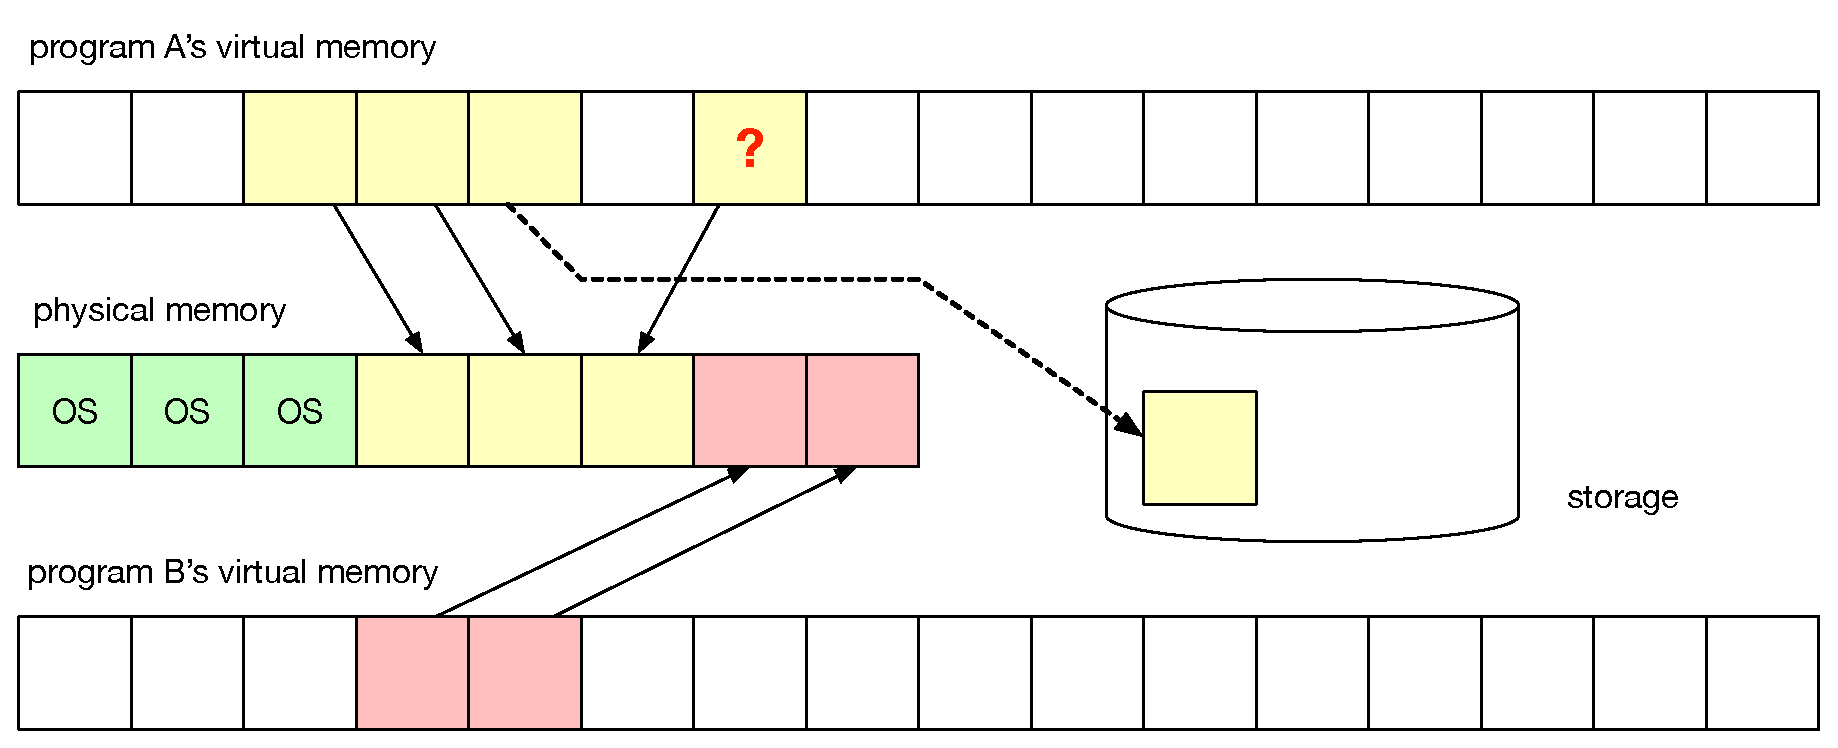
\includegraphics[width=\textwidth]{figures/virtual_memory_scene3.eps}
\end{center}

\vskip1em

The OS takes a page from main memory and \textbf{swaps it out} to storage. This is easy to do because disk blocks and pages have the same size\footnote{Or one is a multiple of the other.}

\end{frame}

%
% ---------------------------------------------------------------------------
%

\begin{frame}

What if a program reads/writes a virtual page that has been swapped out?

\vskip1em

\begin{center}
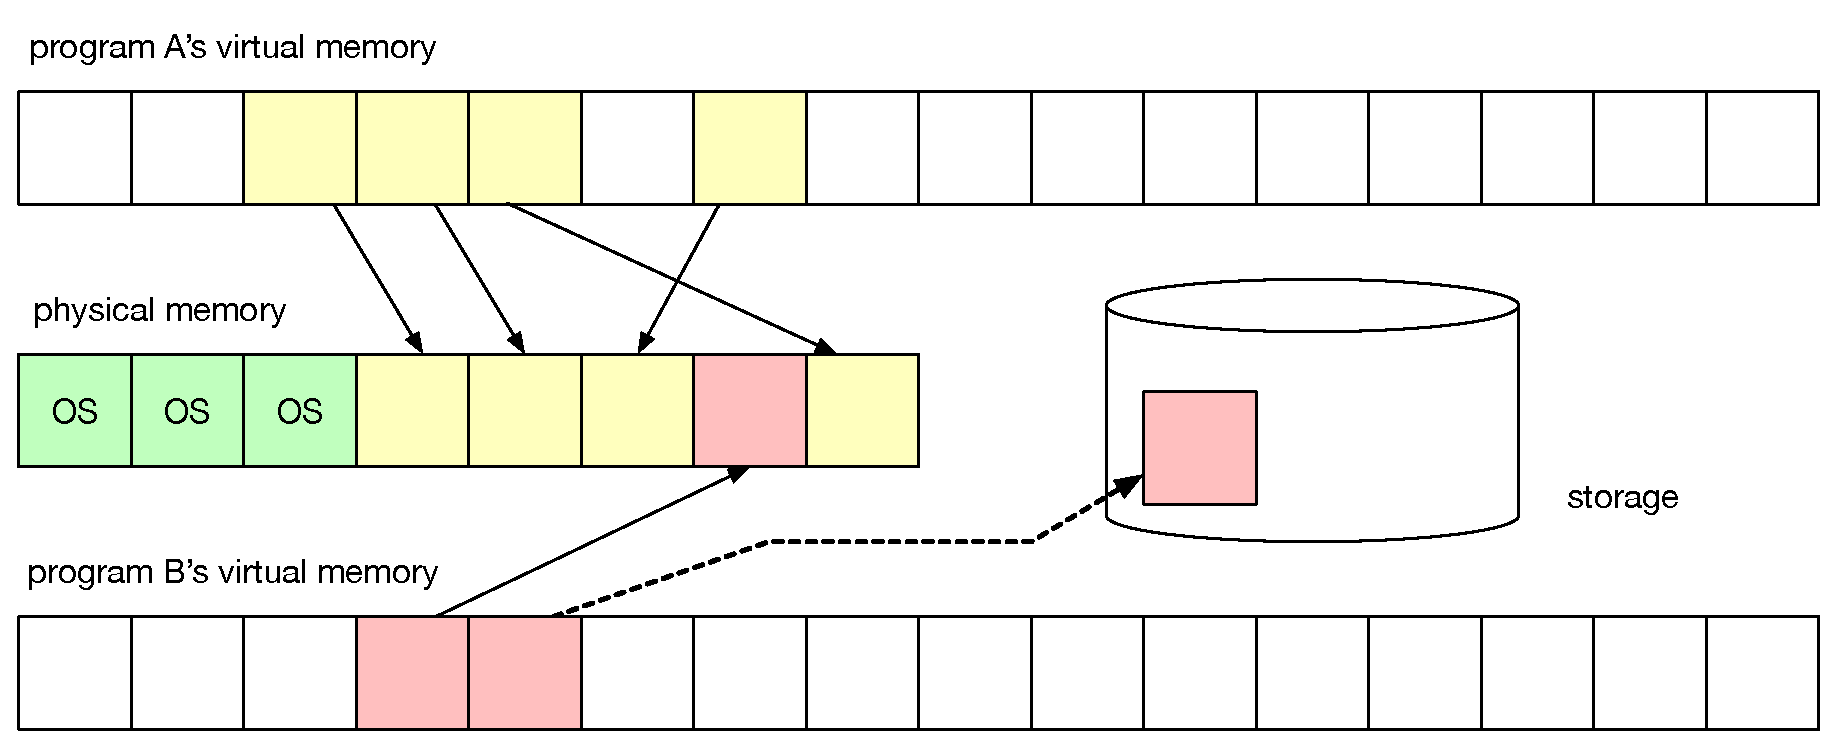
\includegraphics[width=\textwidth]{figures/virtual_memory_scene4.eps}
\end{center}

\vskip1em

The OS takes another page from main memory, \textbf{swaps it out} to storage, making room to \textbf{swap in} the page that was on disk.

\end{frame}


%
% ---------------------------------------------------------------------------
%
\begin{frame}

Recap:
\begin{enumerate}[(1),noitemsep,topsep=-0.5em]
\item Programs always use virtual addresses.
\item The OS places virtual pages into physical pages in memory.
\item The OS moves pages in and out of memory to keep the programs running.
\end{enumerate}

\vskip1em

Recall that memory addresses have 2 parts: $m$ bits for the page, $n$ bits for the offset.

Because virtual and physical pages have the same size, the ``offsets'' in the memory addresses remain unchanged, so all we need to do is to translate ``page'' portion of the address.
\end{frame}

%
% ---------------------------------------------------------------------------
%

\begin{frame}
\label{virtual_memory_size}

The ``size'' of virtual memory in a modern 64-bit CPU is 16 exabytes! No single computer with that much memory exists (and it is unlikely one will ever be built). 

It is common for hardware manufacturers to use fewer bits for physical addresses, based on practical limits.

In any case, the translation of virtual to physical pages considers only the ``page'' part of the address.

\vskip1em

\begin{columns}[onlytextwidth]
\begin{column}{0.6\textwidth}
Example of a modern AMD CPU:

\begin{itemize}[-,noitemsep,topsep=-1em]
\item 64-bit virtual addresses (16 EB)
\item 4KB pages (12 bit offsets)
\item 48-bit real addresses (256 TB\footnotemark)
\end{itemize}
\end{column}
\begin{column}{0.4\textwidth}
\hspace*{-1em}
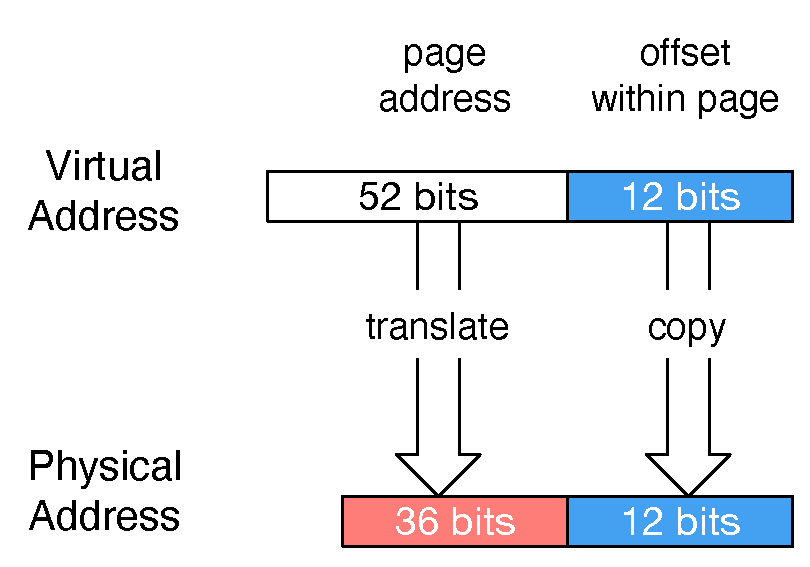
\includegraphics[width=\textwidth]{figures/TLB_translation.eps}
\end{column}
\end{columns}

\footnotetext{Note that this is the maximum allowed.}

\end{frame}

%
% ---------------------------------------------------------------------------
%

\begin{frame}{Implementing Virtual Memory}


Translating virtual page addresses into real page addresses needs to be done fast, and is accomplished with the help of dedicated circuits.

\vskip1em


\begin{BOX}{Virtual Memory Implementation}
\begin{itemize}[-,itemsep=-10pt]
\item the Operating Systems keeps a \textbf{Page Table} mapping virtual pages to real pages;\\

\item the CPU keeps a \emph{cache} of the table in special hardware called \textbf{Translation Lookaside Buffer (TLB)}\\

\item every program has its own page table and TLB entries
\end{itemize}
\end{BOX}

\end{frame}


%
% ---------------------------------------------------------------------------
%
\begin{frame}
\vskip2em
\begin{columns}[onlytextwidth]
\begin{column}{0.4\textwidth}
\textbf{Q:} \alert{\textbf{Which} page(s) should the OS swap out} when needed?

\vskip0.5em

\textbf{A:} Pages that have not been used in a while would be best.

\end{column}
\begin{column}{0.6\textwidth}
\hspace*{1em}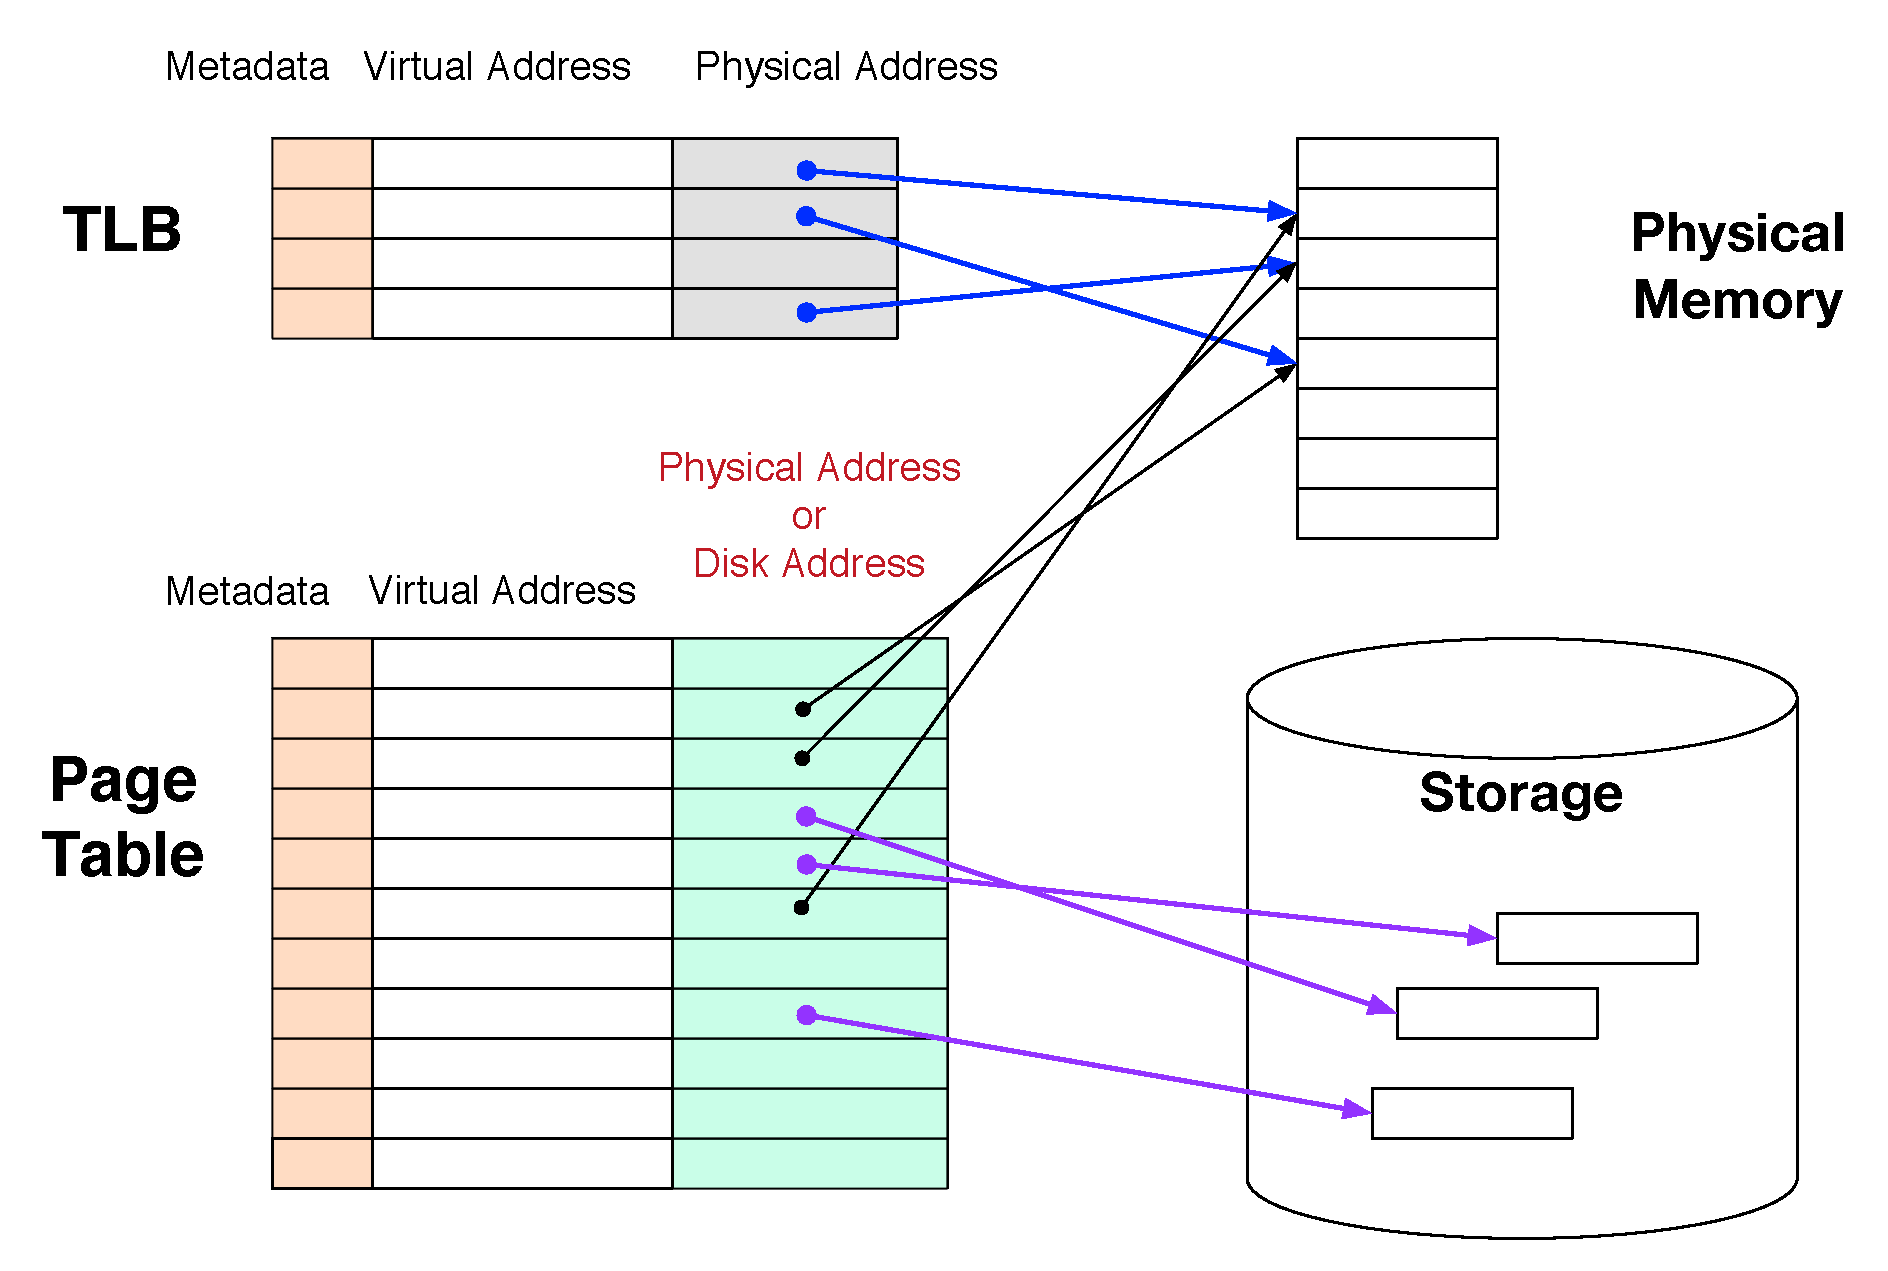
\includegraphics[width=\textwidth]{figures/virtual_memory_TLB.eps}
\end{column}
\end{columns}

\vskip0.5em



The \textbf{metadata} fields in the page table and the TLB keep this kind of information, which the Operating System uses to decide which page to evict.
\end{frame}

%
% ---------------------------------------------------------------------------
%





%
% ============================================================================
%
\section{The role of the Operating System}
%!TEX root = ./lec03_hardware.tex

\begin{frame}

\begin{block}{definition}
An \textbf{operating system (OS)} is system software that manages computer hardware, software resources, and provides common services for computer programs.\footnotemark
\end{block}

\footnotetext{\url{https://en.wikipedia.org/wiki/Operating_system}}

\vskip1em

The OS is responsible for ensuring that applications don't interfere with one another and that all applications and users have a fair share of the computing resources.

To do that, the OS acts as the arbiter that gives and takes access to resources, as needed.

\end{frame}

\begin{frame}

In a modern multi-tasking OS, each application is executed by one or more \textbf{processes}. 

\begin{center}
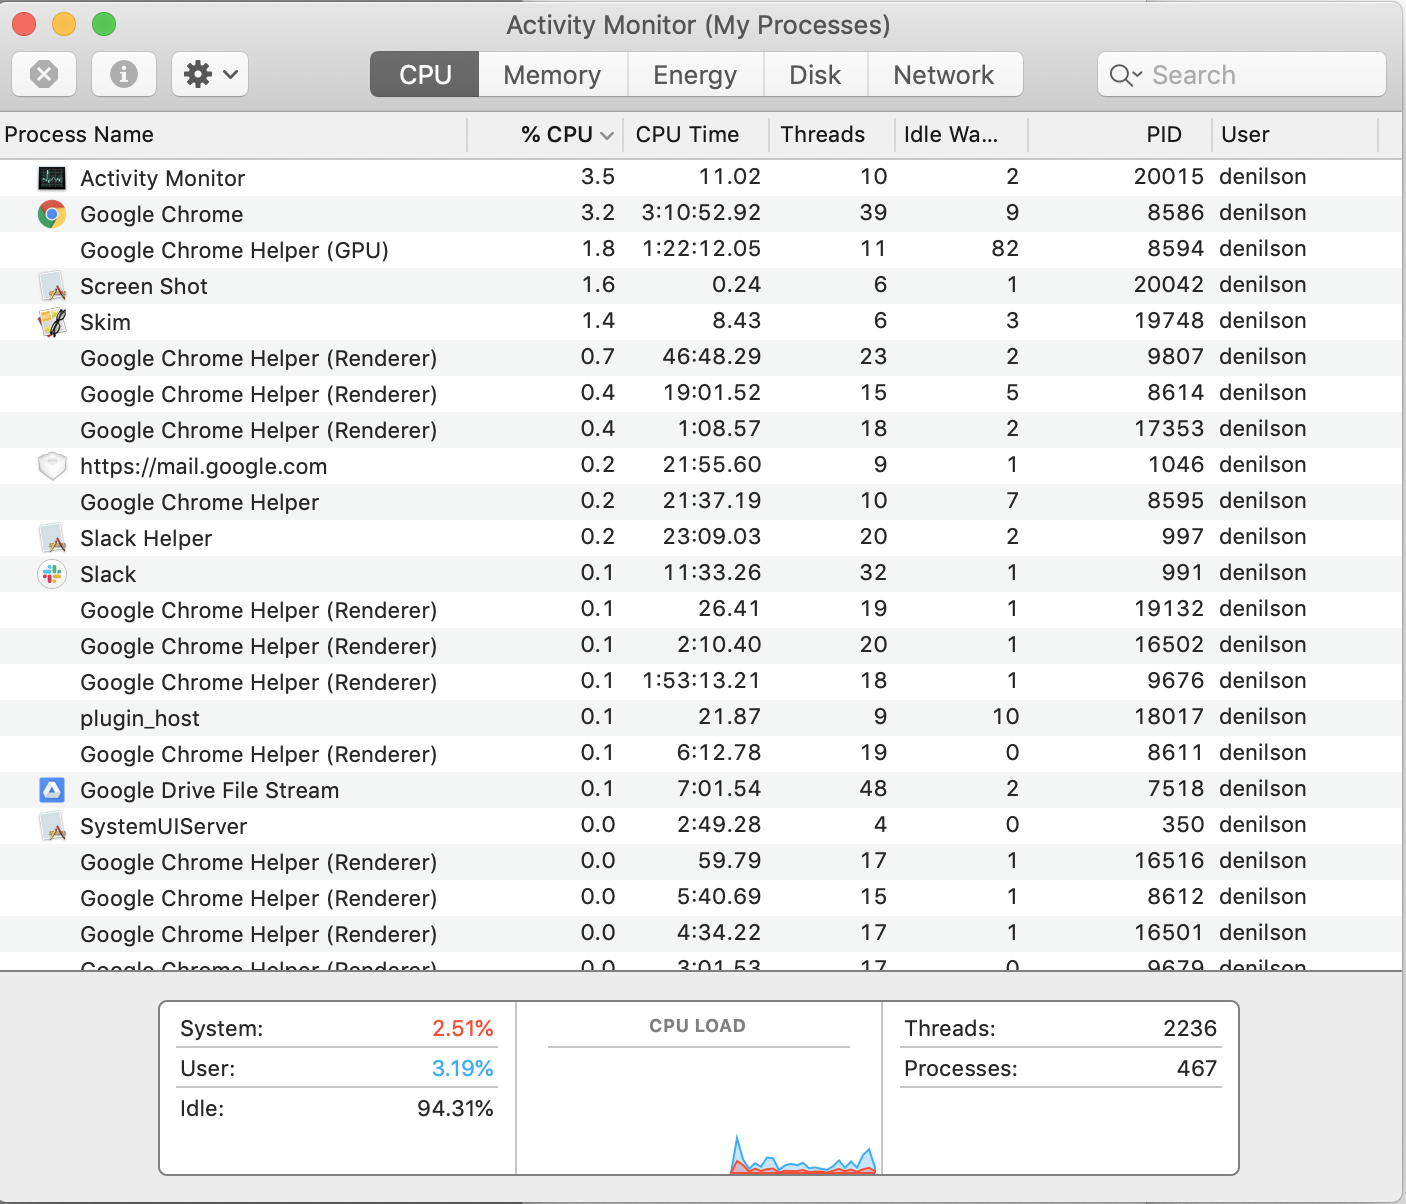
\includegraphics[width=0.75\textwidth]{figures/Activity_Monitor.png}
\end{center}

\end{frame}

\begin{frame}

Processes cannot interfere with one another, meaning:
\begin{itemize}[-, noitemsep]
\item Each user process has its own (virtual) memory buffers and its own files.
\item No process can read/write buffers (and files) ``owned'' by another user/application.
\end{itemize}

\vskip2em

The OS, however, can swap (in/out) data memory buffers of any process as needed.

\vskip1em 

The OS gives the \alert{illusion of real time parallel execution} of multiple processes by constantly swapping processes in/out of the CPU.

\end{frame}


\begin{frame}

What does this have to do with databases?

A DBMS is a complex application, that is implemented by \textbf{many} processes:
\begin{itemize}[-, noitemsep]
\item In some systems, each user query is executed by a separate OS process (normally owned by the same OS user).
\item Often, there will be processes for each user connection in a multi-user system.
\item At least, each large module of the DBMS is implemented by a different process (e.g., query processing, backups, logging, indexing, ...).
\end{itemize}
\end{frame}

\begin{frame}

Over-simplified view of the various OS processes comprising a DBMS:


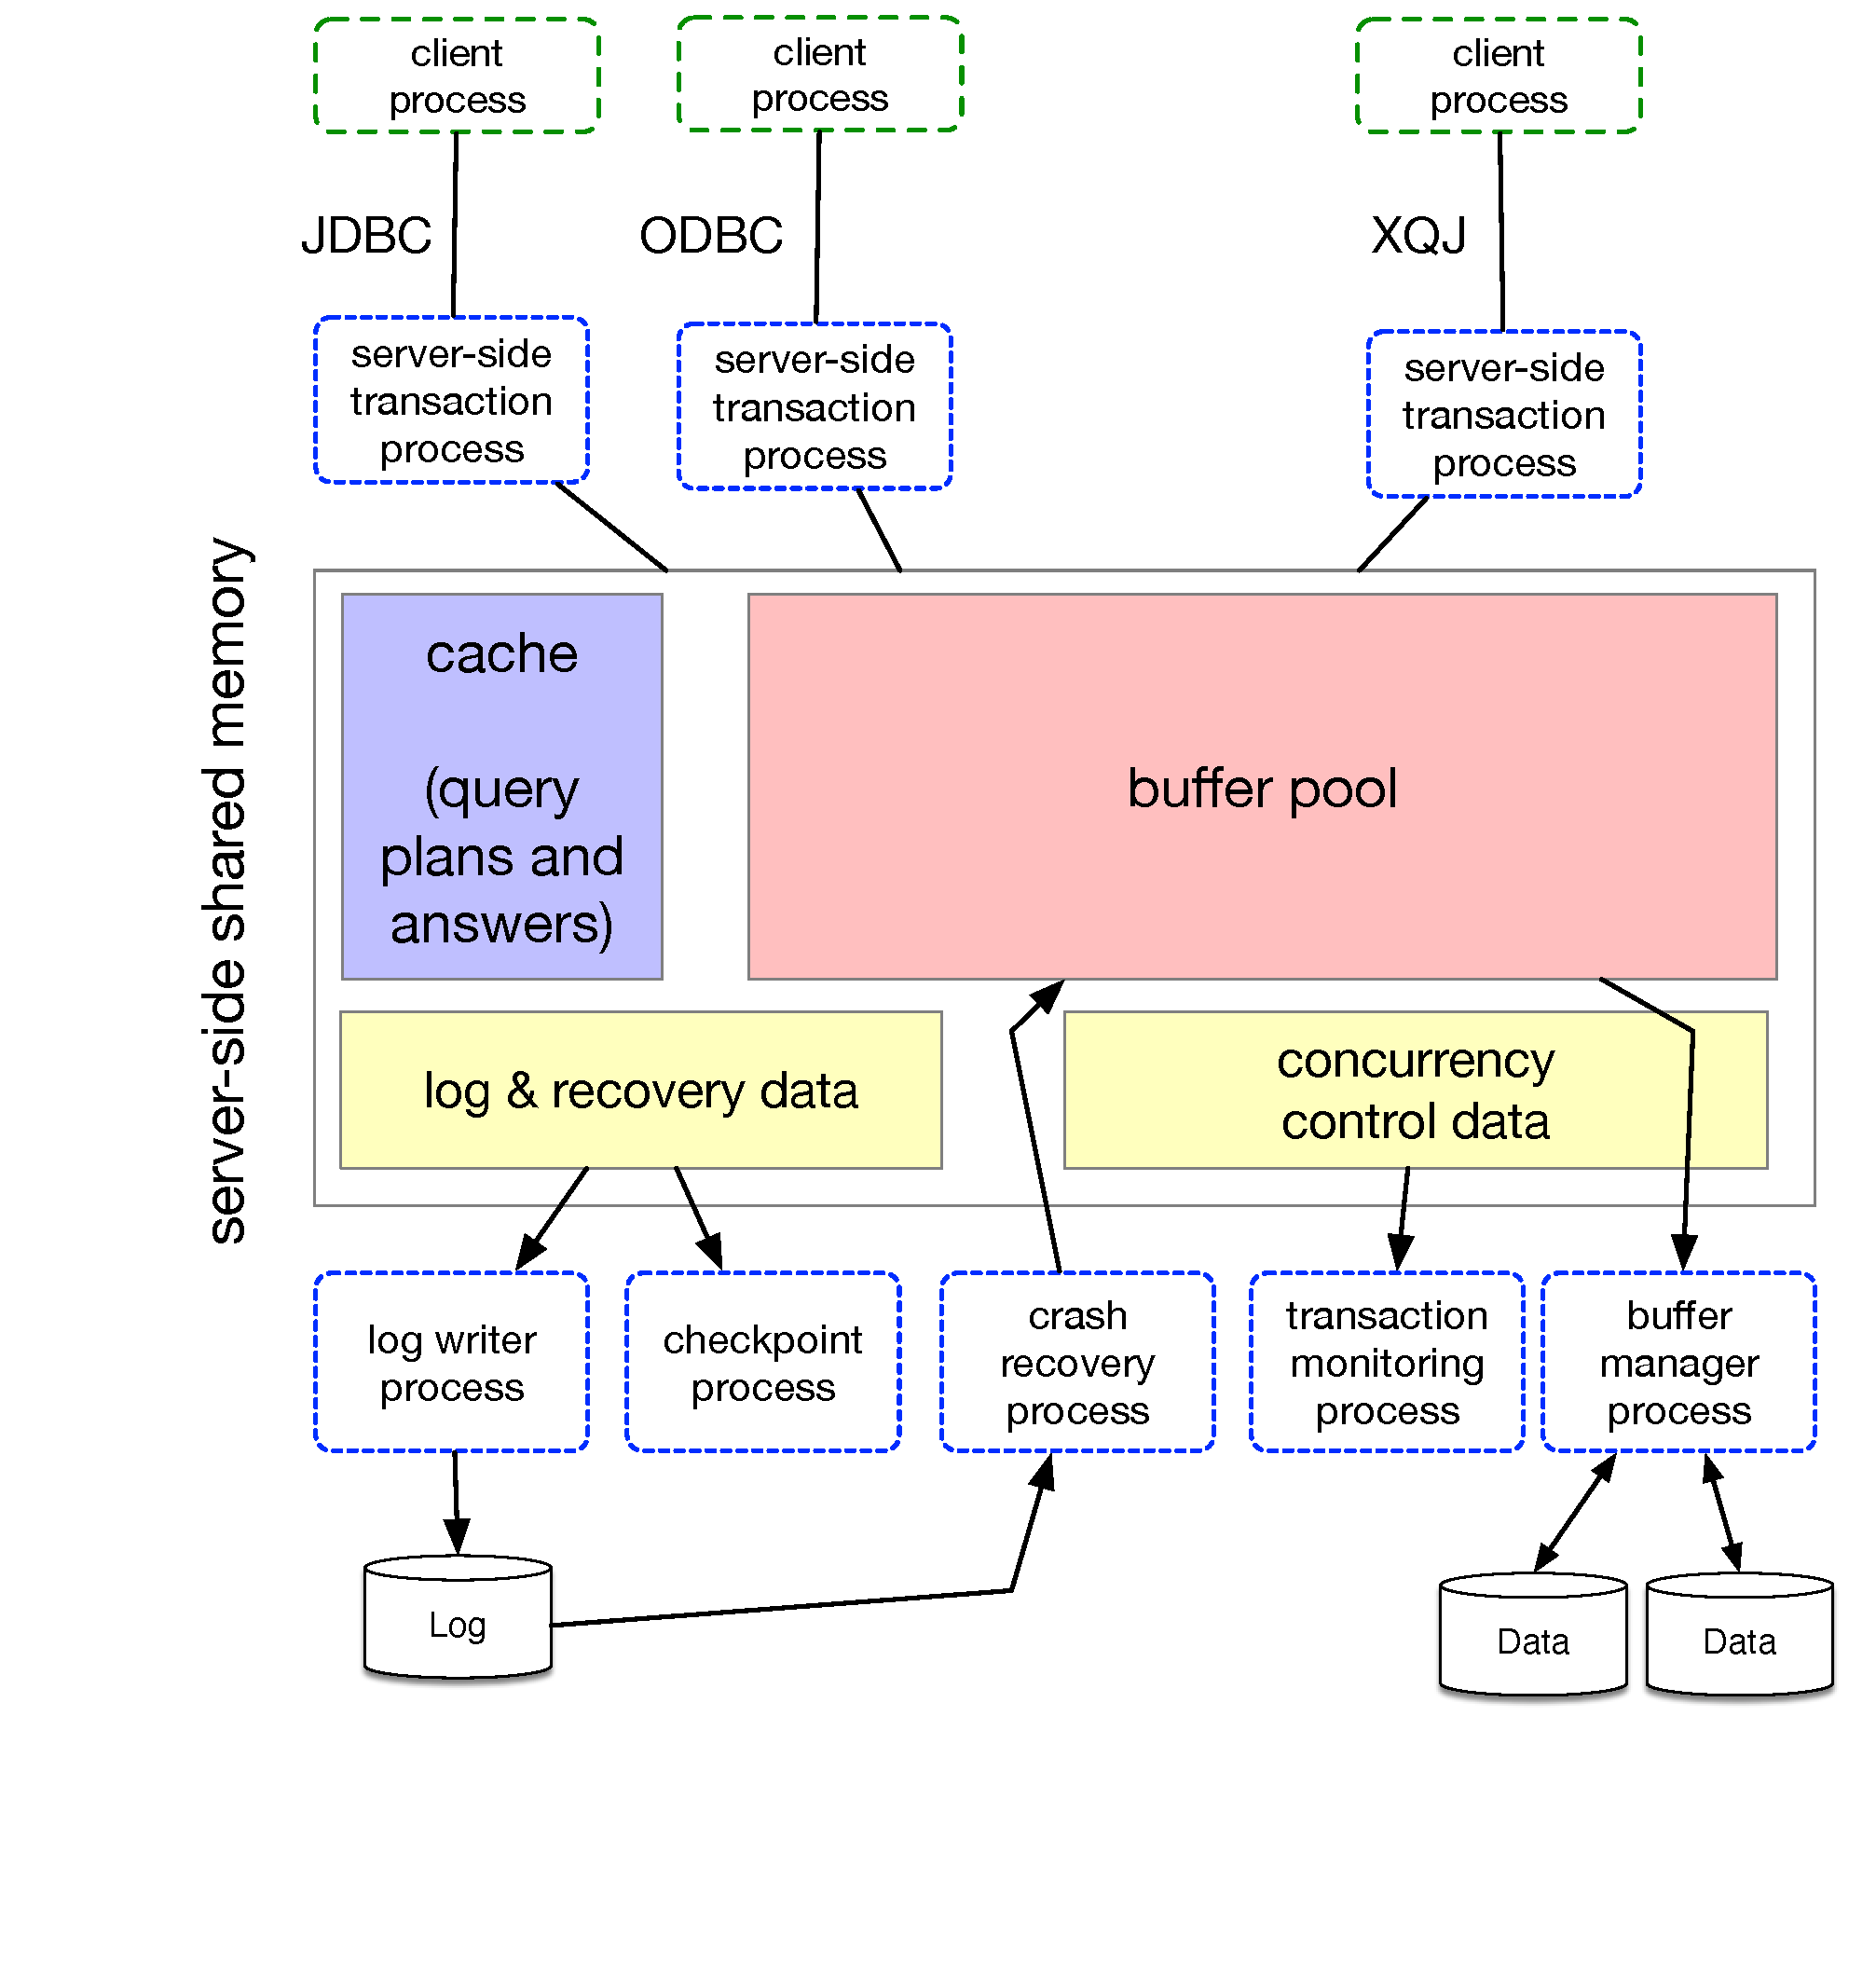
\includegraphics[width=0.8\textwidth]{figures/processes_memory_disks.eps}

\end{frame}


%
% ============================================================================
%
\section{DBMS Architecture Considerations}
%!TEX root = ./lec03_hardware.tex

%
% ---------------------------------------------------------------------------
%
\begin{frame}{DBMS Operational Requirements}


\vskip2em

The DBMS must meet these conflicting goals:

\vskip1em

\begin{columns}[onlytextwidth]
\begin{column}{0.475\textwidth}
\begin{BOX}{Preserving data}
To \textbf{preserve the data}, the DBMS must make sure that it is safely stored in persistent storage\footnotemark.
\end{BOX}
\end{column}
\begin{column}{0.475\textwidth}
\begin{BOX}{Using data}
Queries and updates are processed by the CPU!\\
 - the data needs to reach the registers
\end{BOX}
\end{column}
\end{columns}

\vskip1em

As a result: \alert{data is always on the move}.


\footnotetext{In fact, the privacy-conscious should note that it can be \emph{very hard} to erase data that has been properly written into persistent storage.}

\vskip2em
\end{frame}

%
% ---------------------------------------------------------------------------
%
\begin{frame}{How can the DBMS use persistent storage?}

\textbf{Option \#1}: via a File System:\footnote{\url{https://en.wikipedia.org/wiki/File_system}}\\
- there are many good file systems out there;\\
- however, they are optimized to handle a \emph{large number of small files}, logically organized into hierarchies (directories); databases typically have a \emph{small number of large tables}.

% \vskip1em

\textbf{Option \#2}: implementing \highlight{its own} I/O management:\\
- the Buffer Manager reads/writes directly from/to the device;\\
- requires integration with the Operating System kernel.\footnote{\url{https://en.wikipedia.org/wiki/Kernel_(operating_system)}}

\vskip0.5em

\underline{Most DBMSs have their own I/O stack}, and some require changing the Operating System to work.
\end{frame}


%
% ---------------------------------------------------------------------------
%
\begin{frame}

\begin{columns}[onlytextwidth]
\begin{column}{0.75\textwidth}
\vskip2em
\begin{BOX}{The Buffer Manager}

DBMS module responsible for moving data between storage and memory.

\vskip0.5em

It splits main memory into logical units called \emph{buffers}, which are often the same size of a memory page.
\end{BOX}
\vskip1em

Before data becomes visible to the CPU, it must be \emph{copied} in every level of the memory hierarchy!

\vskip1em
Because I/O is so slow, a badly designed Buffer Manager can make the DBMS unusable.
\end{column}
\begin{column}{0.2\textwidth}
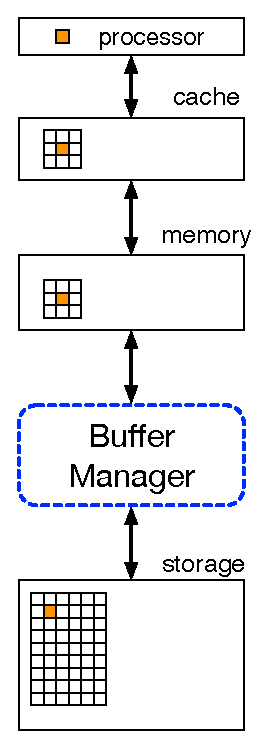
\includegraphics[width=\textwidth]{./figures/buffer_manager}
\end{column}
\end{columns}
\end{frame}

%
% ---------------------------------------------------------------------------
%
\begin{frame}
\begin{columns}[onlytextwidth]
\begin{column}{0.75\textwidth}
\vskip2em
\begin{BOX}{Updates}
When the processor changes an attribute of a tuple, the new value is modified in the cache and the memory first.
\end{BOX}

\vskip0.5em

\begin{BOX}{Insertions}
When a new tuple is inserted, it is stored in some buffer in memory first.\\
 -if there is no room in any buffer, a \emph{new one is created} in memory first.
\end{BOX}

\vfill

Any buffer containing data not yet on the storage layer is said to be \highlight{dirty}.
\end{column}
\begin{column}{0.2\textwidth}
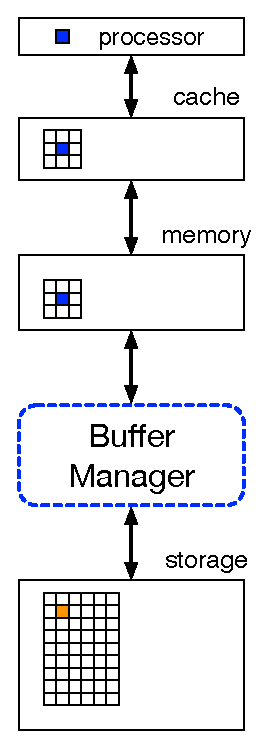
\includegraphics[width=\textwidth]{./figures/buffer_manager_2}
\end{column}
\end{columns}
\end{frame}

%
% ---------------------------------------------------------------------------
%
\begin{frame}

\vskip2em

\begin{BOX}{Dirty data sits in volatile memory}
The Buffer Manager must \alert{\emph{flush} dirty buffers} to the storage layer for the changes to become persistent.
\end{BOX}

\vskip1em

Trade-off:
\begin{itemize}[-,topsep=-0.5em,noitemsep]
\item Because storage is so slow, it is a bad idea to flush dirty buffers \underline{immediately} after every insert/update.
\item The changes to the database do not become permanent \alert{until} they are written on persistent storage.
\end{itemize}



\end{frame}

%
% ---------------------------------------------------------------------------
%
\begin{frame}{Logging, Persistence and Recovery}

\vskip1em

\begin{columns}[onlytextwidth]
\begin{column}{0.6\textwidth}
The DBMS keeps a log of every modification (insertion, deletion, update) done to the database, \emph{on a separate} file (or even a separate storage device).

\vskip1em

Dirty buffers can safely remain in memory as soon as the changes are written to the log.

\vskip1em

If the computer crashes, all changes still in memory can be recovered from the log.
\end{column}
\begin{column}{0.4\textwidth}
\hspace*{2em}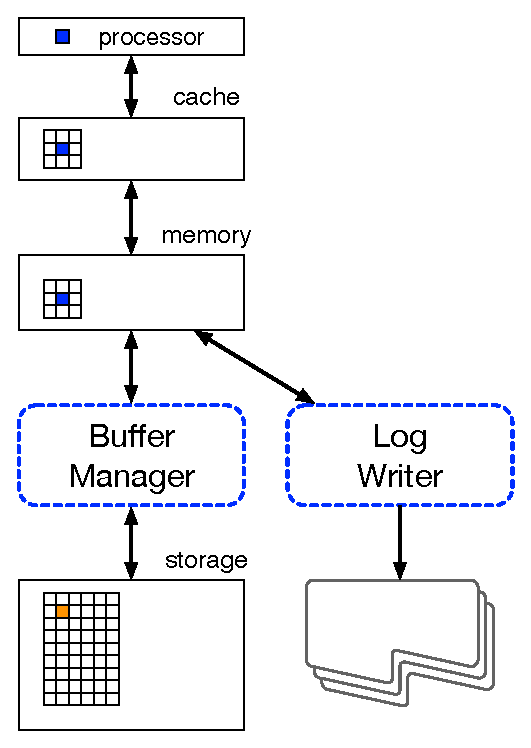
\includegraphics[width=\textwidth]{figures/buffer_manager_log_writer.eps}
\end{column}
\end{columns}
\end{frame}



%
% ---------------------------------------------------------------------------
%
% ---------------------- get the tuplex from the example tables

\newsavebox\MovieI
\savebox{\MovieI}{
	\clipbox{0 45.125 0 22.125}{\usebox\MovieTable}
}
\newsavebox\MovieII
\savebox{\MovieII}{
	\clipbox{0 33.75 0 33.45}{\usebox\MovieTable}
}
\newsavebox\MovieIII
\savebox{\MovieIII}{
	\clipbox{0 22.65 0 44.75}{\usebox\MovieTable}
}
\newsavebox\MovieIV
\savebox{\MovieIV}{
	\clipbox{0 11.3 0 56}{\usebox\MovieTable}
}
\newsavebox\MovieV
\savebox{\MovieV}{
	\clipbox{0 0 0 67.25}{\usebox\MovieTable}
}

\newsavebox\MovieVI
\savebox{\MovieVI}{
	\clipbox{0 0 0 33.5}{\usebox\MovieTableTWO}
}

\def\movieTupleGHOSTBUSTERSone{\scalebox{0.75}{\usebox{\MovieI}}}
\def\movieTupleBIG{\scalebox{0.75}{\usebox{\MovieII}}}
\def\movieTupleLOSTinTRANSLATION{\scalebox{0.75}{\usebox{\MovieIII}}}
\def\movieTupleWADJDA{\scalebox{0.75}{\usebox{\MovieIV}}}
\def\movieTupleGHOSTBUSTERStwo{\scalebox{0.75}{\usebox{\MovieV}}}
\def\movieTupleGROUNDHOGday{\scalebox{0.75}{\usebox{\MovieVI}}}

\def\idxKeyTitleBIG{\scalebox{0.75}{\clipbox{5 0 140 0}{\usebox\MovieII}}}
\def\idxKeyTitleGHOSTBUSTERSone{\scalebox{0.75}{\clipbox{5 0 140 0}{\usebox\MovieI}}}
\def\idxKeyTitleGHOSTBUSTERStwo{\scalebox{0.75}{\clipbox{5 0 140 0}{\usebox\MovieV}}}
\def\idxKeyTitleLOSTinTRANSLATION{\scalebox{0.75}{\clipbox{5 0 140 0}{\usebox\MovieIII}}}
\def\idxKeyTitleWADJDA{\scalebox{0.75}{\clipbox{5 0 140 0}{\usebox\MovieIV}}}

\def\idxKeyTitleYearBIG{\scalebox{0.75}{\clipbox{8 0 111 0}{\usebox\MovieII}}}
\def\idxKeyTitleYearGHOSTBUSTERSone{\scalebox{0.75}{\clipbox{8 0 111 0}{\usebox\MovieI}}}
\def\idxKeyTitleYearGHOSTBUSTERStwo{\scalebox{0.75}{\clipbox{8 0 111 0}{\usebox\MovieV}}}
\def\idxKeyTitleYearLOSTinTRANSLATION{\scalebox{0.75}{\clipbox{8 0 111 0}{\usebox\MovieIII}}}
\def\idxKeyTitleYearWADJDA{\scalebox{0.75}{\clipbox{8 0 111 0}{\usebox\MovieIV}}}


% -------------------------- macros for drawing tuples in the data file

\tikzset{
	tuple/.style={
		anchor=north west,
		inner sep=0pt,outer sep=0pt,shift={(0pt,-2pt)}
	}
}

\tikzset{ % same as above, except for the anchor part
	tupleBelow/.style={
		inner sep=0pt,outer sep=0pt,shift={(0pt,-2pt)}
	}
}


% #1     --> id of tuple (i.e., the node with the value)
% #2, #3 --> coordinages of top-left corner of node with tuple value
% #4     --> value in the attribute of the tuple
\def\tuple#1#2#3#4{
  \node ({#1}) at ({#2},{#3}) [tuple] {{#4}} ;
}

% #1     --> id of tuple (i.e., the node with the value)
% #2, #3 --> coordinages of top-left corner of node with tuple value
% #4     --> value in the attribute of the tuple
\def\tupleBelow#1#2#3{
  \node ({#1}) [below = -2pt of {#2}] [tupleBelow] {{#3}} ;
}


% --------------------------- macros for drawing blocks of the data file

\tikzset{
	MovieDataBlock/.style={
		draw,rectangle,minimum width=5.5125cm, minimum height=0.69cm,anchor=north west,inner sep=1pt,outer sep=1pt
	}
}

\tikzset{
	MovieDataBlockPointerBox/.style={
		fill=snow,draw,rectangle,minimum width=1em,minimum height=1em,
		anchor=north west,
		inner sep=1pt,outer sep=1pt,
		shift={(5.5125cm,-0.34cm)}
	}
}


% #1    --> block id
% #2,#3 --> coordinates of top-left corner
% #4    --> id of the first tuple
% #5    --> value of the first tuple
\def\movieDataBlock#1#2#3#4#5{
	\node ({#1}) at ({#2},{#3}) [MovieDataBlock] {};
	\node at ({#2},{#3}) [MovieDataBlockPointerBox] {};
	
	\tuple{#4}{#2}{#3}{#5};
}

% #1     --> block id
% #2     --> id of block ``above'' this one
% #3, #4 --> coordinates of this block
% #5     --> id of the first tuple inside the block
% #6     --> value of the first tuple
\def\movieDataBlockBelow#1#2#3#4#5#6{
	\node ({#1}) at ({#3},{#4}) [MovieDataBlock] {};
	\node at ({#3},{#4}) [MovieDataBlockPointerBox] {};
	\draw [*->] ([xshift=4pt,yshift=8pt]{#2}.south east) to[out=270,in=90] ([xshift=-10pt]#1.north east);

	\tuple{#5}{#3}{#4}{#6};
}


% --------------------------- macros for drawing the keypointer pairs in the index

\tikzset{
	indexKeyBox/.style={
		anchor=north west,
		inner sep=0pt,outer sep=0pt,shift={(2pt,-2pt)}
	}
}

\tikzset{ %same as above, except for the anchor point
	indexKeyBelowBox/.style={ 
		inner sep=0pt,outer sep=0pt
	}
}

\tikzset{
	indexPointerBox/.style={
		fill=snow,draw,rectangle,minimum width=0.75cm,minimum height=0.3cm,
		inner sep=1pt,outer sep=1pt
	}
}

% draws two rectangles, one with an attribute value, the other with the pointer
%
% #1     --> id of key-pointer (i.e., the node with the value)
% #2, #3 --> coordinages of top-left corner of node with tuple value
% #4     --> value in the attribute of the tuple
\def\movieIndexKeyPointer#1#2#3#4{
  \node ({#1}) at ({#2},{#3}) [indexKeyBox] {#4} ;
  \node [right = -0.5pt of {#1}] [indexPointerBox] {};
}

% #1     --> id of key-pointer (i.e., the node with the value)
% #2     --> id of key-pointer immediately above
% #4     --> value in the attribute of the tuple
\def\movieIndexKeyPointerBelow#1#2#3{
  \node ({#1}) [below = -0.5pt of {#2}] [indexKeyBelowBox] {\tiny{#3}} ;
  \node [right = -0.5pt of {#1}] [indexPointerBox] {};
}


% --------------------------- macros for drawing blocks of the index file

\tikzset{
	MovieIndexBlock/.style={
		draw,rectangle,anchor=north west,inner sep=1pt,outer sep=1pt
	}
}

\tikzset{
	MovieIndexBlockPointerBox/.style={
		fill=snow,draw,rectangle,minimum height=1em,minimum width=1em,
		anchor=north west,
		inner sep=0pt,outer sep=0pt
	}
}

% #1    --> block id
% #2,#3 --> coordinates of top-left corner
% #4    --> WIDTH of block box
% #5    --> HEIGHT of the block box
% #6    --> id of the key-pointer pair
% #7    --> value of the first key-pointer pair
\def\movieIndexBlock#1#2#3#4#5#6#7{
	\node ({#1}) at ({#2},{#3}) [minimum width={#4},minimum height={#5},MovieIndexBlock] {};
	\node [below left= 0pt and 0pt of {#1}] [shift={(-0.9em,1.1em)},MovieIndexBlockPointerBox] {};

	\movieIndexKeyPointer{#6}{#2}{#3}{#7};
}

% #1    --> block id
% #2    --> id of block above
% #3,#4 --> coordinates of top-left corner
% #5    --> WIDTH of block box
% #6    --> HEIGHT of the block box
% #7    --> id of the key-pointer pair
% #8    --> value of the first key-pointer pair
\def\movieIndexBlockBelow#1#2#3#4#5#6#7#8{
	\node ({#1}) at ({#3},{#4}) [minimum width={#5},minimum height={#6},MovieIndexBlock] {};
	\node [below left= 0pt and 0pt of {#1}] [shift={(-0.9em,1.1em)},MovieIndexBlockPointerBox] {};
	\draw [*->] ([xshift=-0.4em,yshift=0.8em]{#2}.south west) to[out=270,in=90] ([xshift=10pt]{#1}.north west);

	\movieIndexKeyPointer{#7}{#3}{#4}{#8};
}


% ----------------------------- draw line between pointer into tuple

% #1 --> key-pointer id
% #2 --> tuple id
\def\KPtoTuple#1#2{
	\draw [*->] ([xshift=0.35cm,yshift=0em]{#1}.east) to[out=0,in=180] (#2.west);
}

% ======================== actual examples

\newsavebox\TitleIndexOnMovie
\savebox{\TitleIndexOnMovie}{
\begin{tikzpicture}
\movieDataBlock{Mdb1}{0}{0}{t1}{\movieTupleGHOSTBUSTERSone};
\tupleBelow{t2}{t1}{\movieTupleBIG};
\movieDataBlockBelow{Mdb2}{Mdb1}{0}{-1.25}{t3}{\movieTupleLOSTinTRANSLATION};
\tupleBelow{t4}{t3}{\movieTupleWADJDA};
\movieDataBlockBelow{Mdb3}{Mdb2}{0}{-2.5}{t5}{\movieTupleGHOSTBUSTERStwo};

\movieIndexBlock{MIb1}{-4.5}{0}{7.6em}{3.6em}{kp1}{\idxKeyTitleBIG};
\movieIndexKeyPointerBelow{kp2}{kp1}{\idxKeyTitleGHOSTBUSTERSone};
\movieIndexKeyPointerBelow{kp3}{kp2}{\idxKeyTitleGHOSTBUSTERStwo};
\movieIndexKeyPointerBelow{kp4}{kp3}{\idxKeyTitleLOSTinTRANSLATION};
\movieIndexBlockBelow{MIb2}{MIb1}{-4.5}{-2.25}{7.6em}{3.6em}{kp5}{\idxKeyTitleWADJDA};

\KPtoTuple{kp2}{t1};
\KPtoTuple{kp1}{t2};
\KPtoTuple{kp4}{t3};
\KPtoTuple{kp5}{t4};
\KPtoTuple{kp3}{t5};
\end{tikzpicture}}


\newsavebox\TitleYearIndexOnMovie
\savebox{\TitleYearIndexOnMovie}{
\begin{tikzpicture}
\movieDataBlock{Mdb1}{0}{0}{t1}{\movieTupleGHOSTBUSTERSone};
\tupleBelow{t2}{t1}{\movieTupleBIG};
\movieDataBlockBelow{Mdb2}{Mdb1}{0}{-1.25}{t3}{\movieTupleLOSTinTRANSLATION};
\tupleBelow{t4}{t3}{\movieTupleWADJDA};
\movieDataBlockBelow{Mdb3}{Mdb2}{0}{-2.5}{t5}{\movieTupleGHOSTBUSTERStwo};

\movieIndexBlock{MIb1}{-4.5}{0}{9.6em}{2.8em}{kp1}{\idxKeyTitleYearBIG};
\movieIndexKeyPointerBelow{kp2}{kp1}{\idxKeyTitleYearGHOSTBUSTERSone};
\movieIndexKeyPointerBelow{kp3}{kp2}{\idxKeyTitleYearGHOSTBUSTERStwo};

\movieIndexBlockBelow{MIb2}{MIb1}{-4.5}{-2.25}{9.6em}{2.8em}{kp4}{\idxKeyTitleYearLOSTinTRANSLATION};
\movieIndexKeyPointerBelow{kp5}{kp4}{\idxKeyTitleYearWADJDA};

\KPtoTuple{kp2}{t1};
\KPtoTuple{kp1}{t2};
\KPtoTuple{kp4}{t3};
\KPtoTuple{kp5}{t4};
\KPtoTuple{kp3}{t5};
\end{tikzpicture}}


\newsavebox\SequentialFileMovieTitleYear
\savebox{\SequentialFileMovieTitleYear}{
\begin{tikzpicture}
\movieDataBlock{Mdb1}{0}{0}{t1}{\movieTupleBIG};
\tupleBelow{t2}{t1}{\movieTupleGHOSTBUSTERSone};
\movieDataBlockBelow{Mdb2}{Mdb1}{0}{-1.25}{t3}{\movieTupleGHOSTBUSTERStwo};
\tupleBelow{t4}{t3}{\movieTupleLOSTinTRANSLATION};
\movieDataBlockBelow{Mdb3}{Mdb2}{0}{-2.5}{t5}{\movieTupleWADJDA};
\end{tikzpicture}}

\newsavebox\SequentialFileMovieTitlYearUpdated
\savebox{\SequentialFileMovieTitlYearUpdated}{
\begin{tikzpicture}
\movieDataBlock{Mdb1}{0}{0}{t1}{\movieTupleBIG};
\tupleBelow{t2}{t1}{\movieTupleGHOSTBUSTERSone};
\movieDataBlockBelow{Mdb2}{Mdb1}{0}{-1.25}{t3}{\movieTupleGHOSTBUSTERStwo};
\tupleBelow{t4}{t3}{\movieTupleGROUNDHOGday};
\movieDataBlockBelow{Mdb3}{Mdb2}{0}{-2.5}{t5}{\movieTupleLOSTinTRANSLATION};
\tupleBelow{t6}{t5}{\movieTupleWADJDA};
\end{tikzpicture}}

\newsavebox\SequentialFileMovieTitlYearUpdatedTWO
\savebox{\SequentialFileMovieTitlYearUpdatedTWO}{
\begin{tikzpicture}
\movieDataBlock{Mdb1}{0}{0}{t1}{\movieTupleBIG};
\tupleBelow{t2}{t1}{\movieTupleGHOSTBUSTERSone};
\movieDataBlockBelow{Mdb2}{Mdb1}{0}{-1.25}{t3}{\movieTupleGHOSTBUSTERStwo};
\movieDataBlockBelow{Mdb3}{Mdb2}{0}{-2.5}{t4}{\movieTupleGROUNDHOGday};
\tupleBelow{t5}{t4}{\movieTupleLOSTinTRANSLATION};
\movieDataBlockBelow{Mdb4}{Mdb3}{0}{-3.75}{t6}{\movieTupleWADJDA};
\end{tikzpicture}}



\begin{frame}{Database ``Files''?}

Tables are collections of records stored on ``files'' (chains of fixed-sized blocks). Indexes help the DBMS find tuples through pointers.


\begin{tikzpicture}
\node [anchor=north west] at (-0.15,0) {\scalebox{0.85}{\usebox\TitleYearIndexOnMovie}};
\node [color=accent] at (1,0.5) {Index File};
\node [color=accent] at (5,0.5) {Table File};
\end{tikzpicture}

A ``database pointer'' identifies the storage device \emph{and} a block address which can be translated into a device-specific address (recall slide~\ref{block_oriented_storage}).

\end{frame}


%
% ---------------------------------------------------------------------------
%
\begin{frame}{Main Memory Databases}

Some DBMSs (including SQLite) are optimized for main memory and use only virtual memory as its address space.

This is rarely a problem, as Virtual Memory can grow to Petabytes (recall Slide~\ref{virtual_memory_size}) with modern computers.

In any case, relying on virtual memory as the database address space simplifies the DBMS architecture a lot. For example ``database'' pointers can be simplified to virtual memory addresses.

Main-memory DBMSs are also optimized for single-user applications (like mobile applications and video games).

\end{frame}


%
% ---------------------------------------------------------------------------
%
\begin{frame}{What about bigger databases?}

A very small number of applications (and organizations) deal with more than a Petabyte. In such cases, we need clusters of high-performance computers and (often) a custom DBMS.

\begin{center}
\begin{tikzpicture}
\node at (0,0) [anchor=south east] {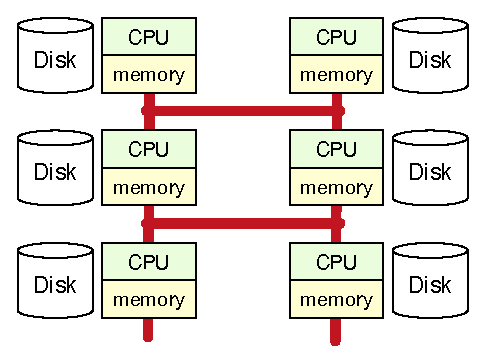
\includegraphics[width=0.4\textwidth]{figures/small_cluster.eps}};
\end{tikzpicture}
\end{center}

In such cases, to identify a tuple we need to know:\\
 - the specific block of a specific storage device holding the tuple\\
 - the IP address of the server with that device (if using a cluster)


\end{frame}


%
% ---------------------------------------------------------------------------
%
\begin{frame}

The standard DBMS implementations use \alert{\textbf{symbolic}} pointers, even for single CPU DBMSs.

Symbolic addresses are typically \underline{much larger} than a memory address. 
Also, symbolic addresses \alert{\textbf{must be resolved}} into virtual memory addresses!

\vskip1.5em

\begin{BOX}{Resolving pointers as blocks are loaded...}
When the Buffer Manager loads a symbolic pointer to memory, it must translate that symbolic address to an actual \emph{virtual memory} address where the target of the link is actually loaded.
\end{BOX}
\end{frame}


%
% ============================================================================
%
\section{Architectures of Database \textbf{Applications}}
%!TEX root = ./lec03_hardware.tex


%
% ---------------------------------------------------------------------------
%
\begin{frame}{Database \textbf{Application} Architecture}

Multi-user applications are best developed as client-server applications.

\begin{block}{\alert{Client-Server} applications}
The DBMS (server) and the application (client) run as independent processes, often on different computers. There usually is one server for many clients.
\end{block}

\vskip1em

Single-user applications (e.g., apps on mobile devices or some games) can be developed as a single process:

\begin{block}{\alert{Embedded DBMS} applications}
The application and the DBMS are \textbf{compiled} together and run as a single process on the same device.
\end{block}


\end{frame}

%
% ---------------------------------------------------------------------------
%
\begin{frame}
\label{client_server_separate}
\textbf{Client-server} on separate computers:

\begin{center}
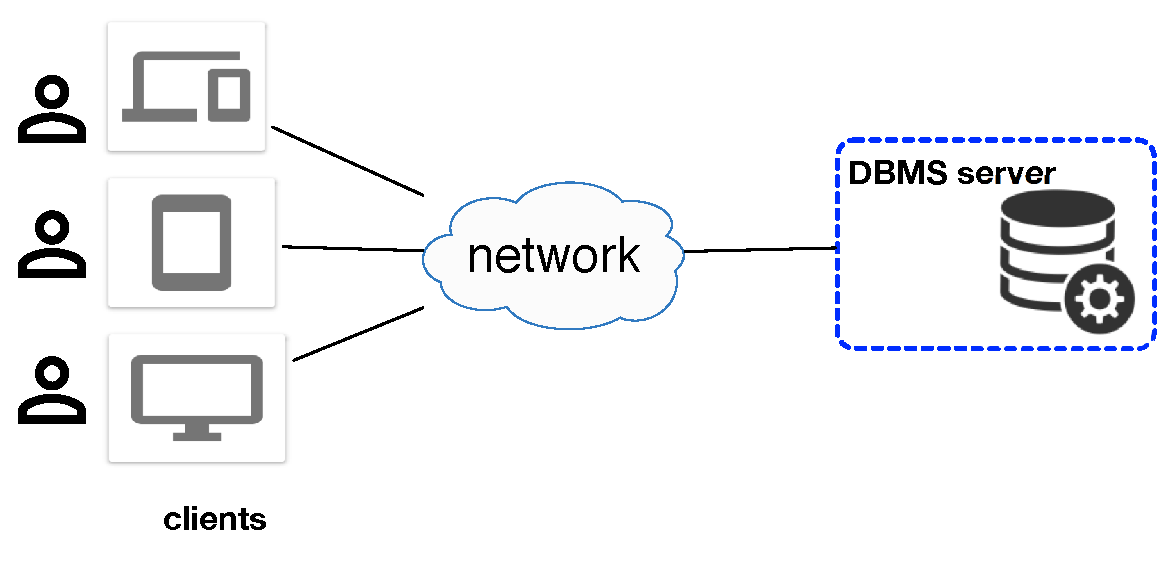
\includegraphics[width=0.75\textwidth]{figures/client_server_cloud}
\end{center}

\textbf{Example: Beartracks} (clients are Web apps on browsers)

\begin{BOX}{Connecting to the server}
The client needs a \emph{connector} API to talk to the DBMS.

\vskip0.5em

ODBC\footnotemark  is widely used for this.
\end{BOX}

\footnotetext{\url{https://en.wikipedia.org/wiki/Open_Database_Connectivity}}
\end{frame}

%
% ---------------------------------------------------------------------------
%
\begin{frame}
\vskip2em
\begin{columns}
\begin{column}{0.6\textwidth}
With this architecture, almost all computation happens on the server.

\vskip0.5em

The client presents results to and takes input from the users.
\end{column}
\begin{column}{0.3124\textwidth}
\hspace*{-1.5em}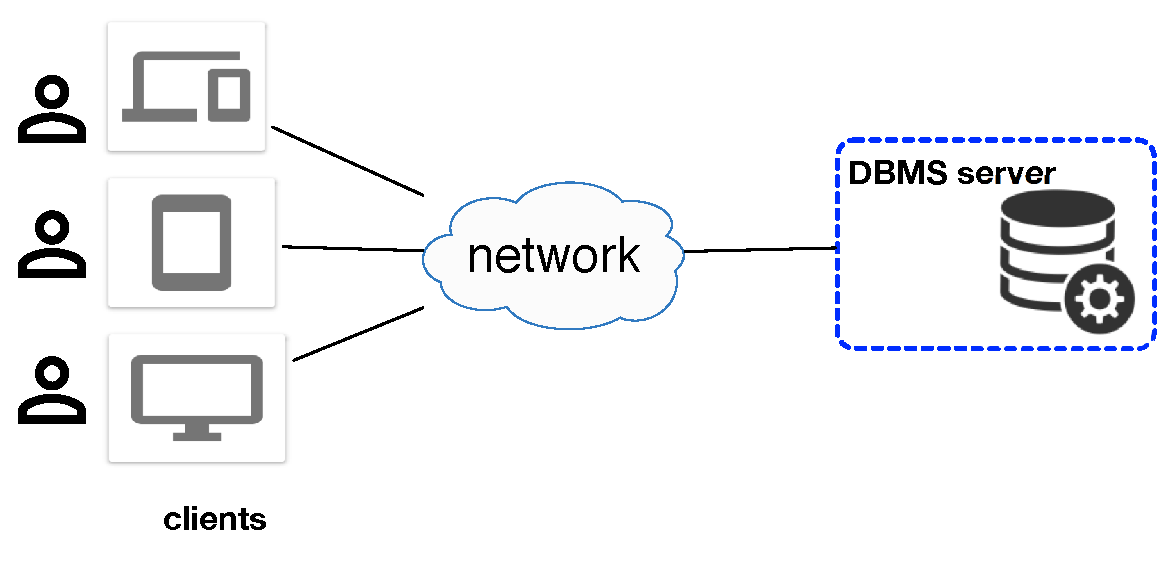
\includegraphics[width=1.25\textwidth]{figures/client_server_cloud}
\end{column}
\end{columns}

\vskip0.5em

Other implications:
\begin{enumerate}[label=(\arabic*)]
\item \underline{scaling} to more users means buying a bigger server
\item all data input/output flows through the \underline{network}
\end{enumerate}
 
This model is best for centralized applications where the provider is responsible for the data (e.g., universities, banks, government agencies, etc.) \textbf{and} where Internet connectivity is a given.

\end{frame}


%
% ---------------------------------------------------------------------------
%
\begin{frame}{Client-Server with DBMS API}

Application developers can use APIs to connect to the DBMS via the network.

\vskip1em

\begin{center}
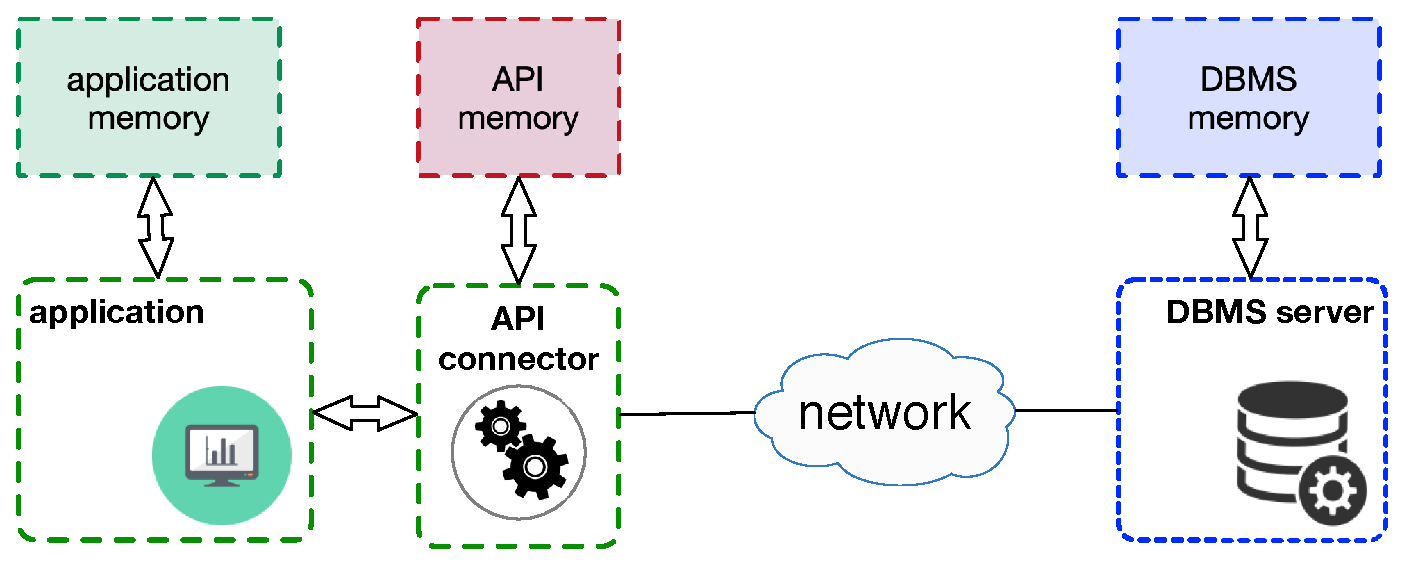
\includegraphics[width=0.6\textwidth]{figures/client_server_API.eps}
\end{center}

\vskip1em

ODBC\footnote{\url{https://en.wikipedia.org/wiki/Open_Database_Connectivity}} (Open Database Connectivity) is an industry standard supported by many languages and DBMS vendors.

\end{frame}


%
% ---------------------------------------------------------------------------
%
\begin{frame}{Client-Server with Embedded SQL}

A more efficient way to deploy a client-server application is to \textbf{embed}\footnote{\url{https://en.wikipedia.org/wiki/Embedded_SQL}} the libraries for connecting to the DBMS within the application itself.

\vskip1em

\begin{center}
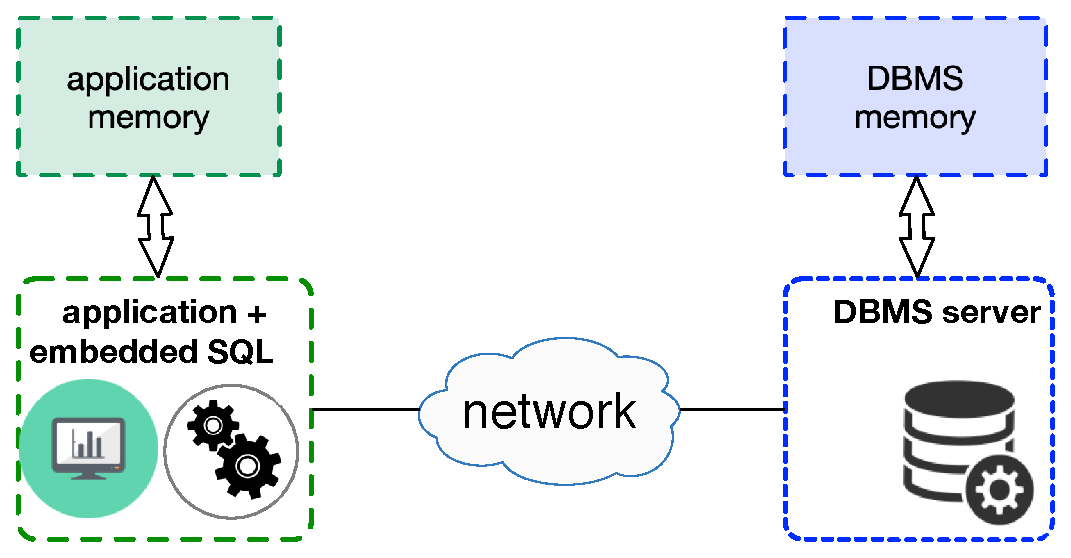
\includegraphics[width=0.6\textwidth]{figures/embedded_SQL_client_server.eps}
\end{center}

\vskip1em

This is done by \textbf{compiling} the application and the libraries together.

\end{frame}


%
% ---------------------------------------------------------------------------
%
\begin{frame}{Client-Server on the same device}

DBMSs are being deployed more and more for \textbf{single-user} applications, e.g., mobile apps or games.

A simple (\alert{but inefficient}) way to do that is to use the standard client-server architecture where both execute as separate processes on the same device:

\vskip1em

\begin{center}
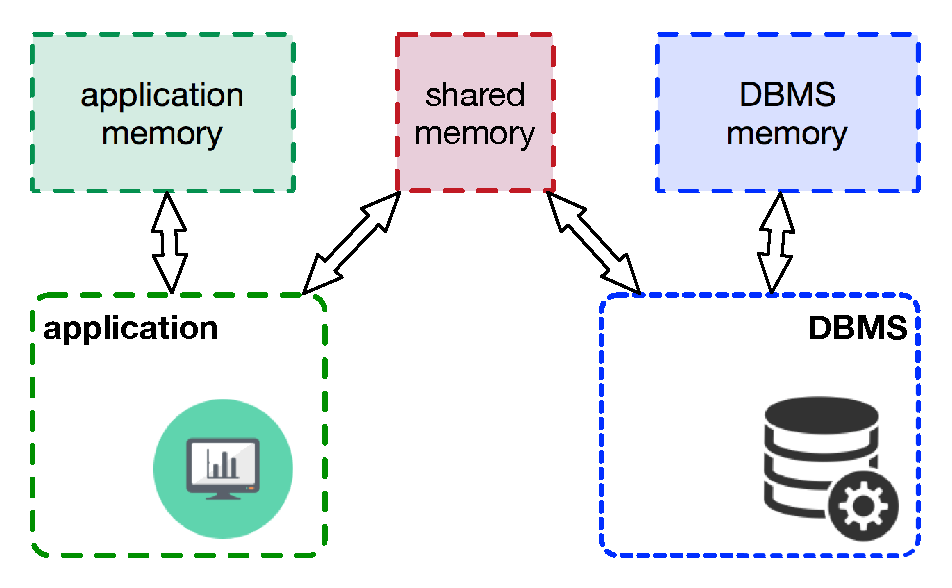
\includegraphics[width=0.6\textwidth]{figures/API_local_system.eps}
\end{center}
\end{frame}



%
% ---------------------------------------------------------------------------
%
\begin{frame}
\vskip2em
\begin{columns}
\begin{column}{0.6\textwidth}

What is so bad about this?

\end{column}
\begin{column}{0.3124\textwidth}
\hspace*{-3.5em}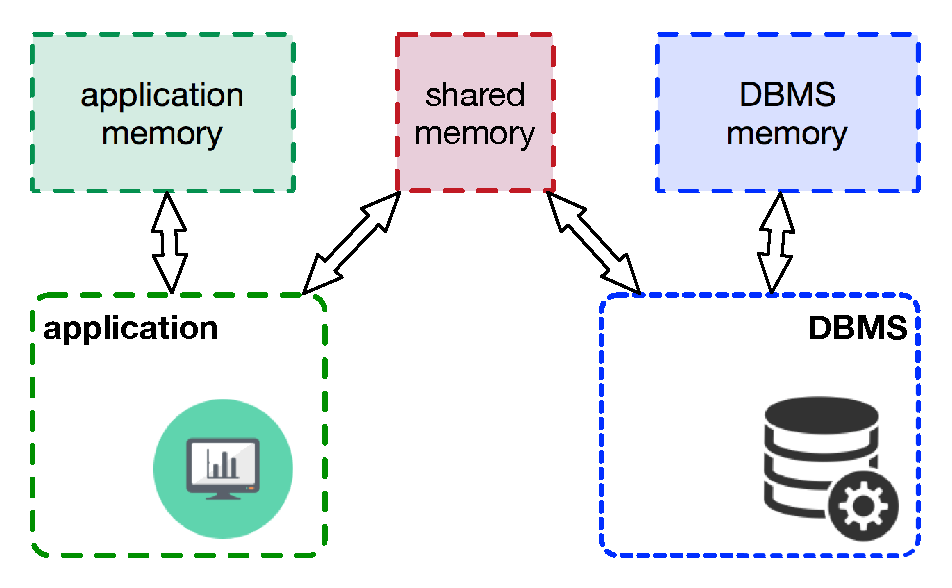
\includegraphics[width=1.25\textwidth]{figures/API_local_system.eps}
\end{column}
\end{columns}

\vskip0.5em

Data must be copied multiple times:\\
 - from storage to DBMS buffers (and back)\\
 - from DBMS buffers to shared pages in memory\footnote{One of the best ways of implementing inter-process communication... Read up \url{https://en.wikipedia.org/wiki/Inter-process_communication}} (and back)\\
 - from shared pages to the application (and back)

This is not only wasteful but also \underline{much slower}:\\
 - even if the computer is \emph{over-provisioned} 

\end{frame}


%
% ---------------------------------------------------------------------------
%
\begin{frame}{Embedded DBMS}

The right way of deploying single-user applications that need DBMS support is to \textbf{embed} the DBMS code inside the application:

\begin{center}
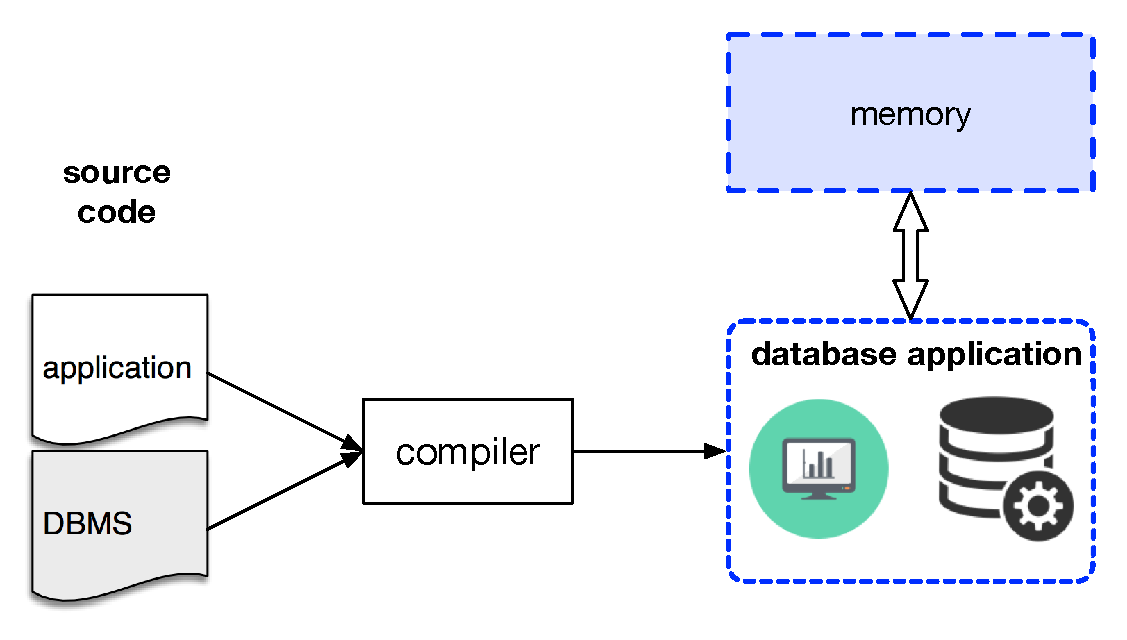
\includegraphics[width=0.6\textwidth]{figures/embedded_dbms_code.eps}
\end{center}

SQLite was designed to be embedded in applications in ANSI C.\footnote{\url{https://sqlite.org/cintro.html}}

\end{frame}


%
% ---------------------------------------------------------------------------
%
\begin{frame}
\vskip2em
\begin{columns}
\begin{column}{0.6\textwidth}

What is so good about this?

\end{column}
\begin{column}{0.3124\textwidth}
\hspace*{-3.5em}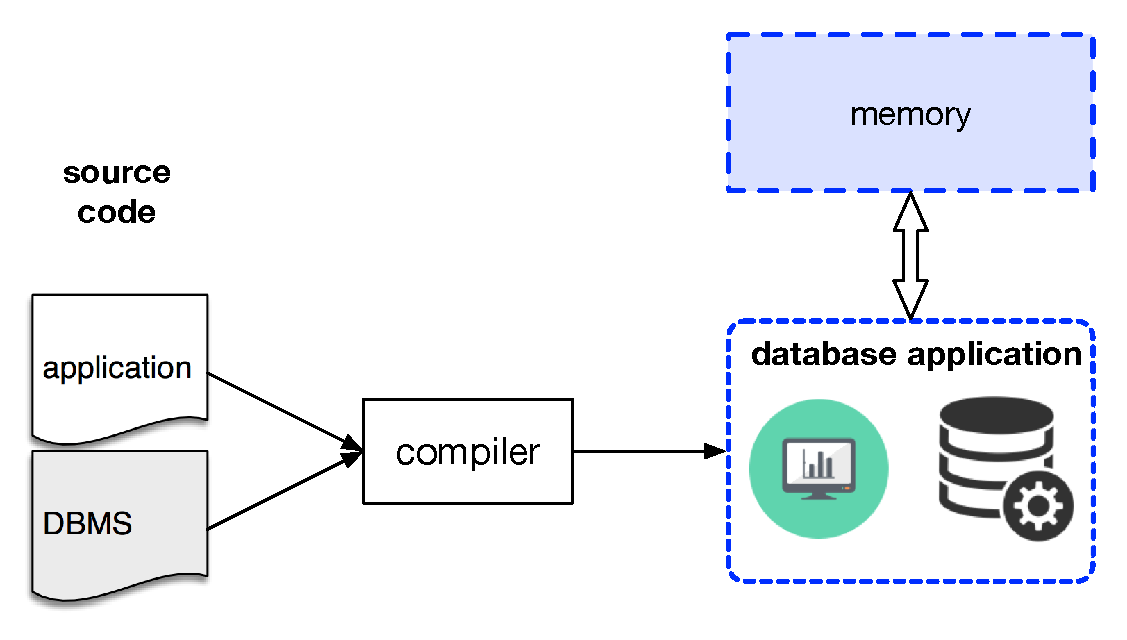
\includegraphics[width=1.25\textwidth]{figures/embedded_dbms_code.eps}
\end{column}
\end{columns}

\vskip0.5em

No copying data around: ``DBMS'' buffers are easily accessible by the ``application''.

Unused/unnecessary components of the DBMS are not compiled into the application, resulting in code with a smaller footprint.

\vskip1em

Embedded data management is a strong trend with mobile apps, computer games, web browsers, etc.

\end{frame}

%
% ---------------------------------------------------------------------------
%
\begin{frame}{ASIDE: embedded SQL in the wild}

Compiling SQL into native code?\\
 - although still a research topic, this is not mad science!\\
 - will be mainstream pretty soon.

Because of its small footprint, efficiency, main-memory option, and its public domain license, SQLite is probably the \textbf{most widely used} relational DBMS in the world today.

Modern MMORPG computer games comprise worlds with thousands of objects which are related in complex ways. Many of them already use relational DBMSs in a client-server mode, and some are moving to an embedded mode.

\end{frame}


%
%
% Further reading/other DBMSs
%
%

%
% ---------------------------------------------------------------------------
%
\begin{frame}{Further references/resources}

Other in-memory/main-memory databases besides SQLite:
\small{\url{https://en.wikipedia.org/wiki/List_of_in-memory_databases}}

\vskip1em

PostgreSQL is an open-source, enterprise-scale client-server DBMSs:
\small{\url{https://www.postgresql.org}}

\vskip1em

Apache Derby is an open-source relational DBMS written in and for Java. It can be efficiently embedded inside Java applications:
\small{\url{http://db.apache.org/derby/}}

\end{frame}



\end{document}